\documentclass[11pt]{article}

% ACL review template. Change "review" to "final" for camera-ready or
% "preprint" for a non-anonymous version with page numbers.
\usepackage[review]{acl}

\usepackage{times}
\usepackage{latexsym}
\usepackage[T1]{fontenc}
\usepackage[utf8]{inputenc}
\usepackage{microtype}
\usepackage{inconsolata}
\usepackage{booktabs}
\usepackage{graphicx}
\usepackage{array}
\usepackage{tabularx}
\usepackage{enumitem}
\usepackage{amsmath}
\usepackage{amsfonts}
\usepackage{amssymb}
\usepackage{forest}
\usepackage{tikz}
\usetikzlibrary{arrows.meta,calc}
\setlength{\emergencystretch}{3em}
\setlength{\linenumbersep}{6pt}

\title{Robust RAG under Unreliable Evidence:\\
A Comparability Framework and Evidence Audit}

\author{Anonymous Authors}
\date{}

\begin{document}
\maketitle

\begin{abstract}
Robust retrieval-augmented generation (RAG) grounds language models in external evidence, but that evidence can be irrelevant, distracting, conflicting, stale, insufficient, or adversarially corrupted. A growing literature reports progress on ``noise robustness'', ``faithfulness'', ``security'', and ``calibration'', yet these results are hard to compare: papers that share a label often differ in their evidence assumptions, interventions, metrics, and---crucially---the action the system is expected to take. We argue that robust-RAG progress should be read through a comparability lens, and we make that lens precise with a five-coordinate tuple: failure type, evidence assumption, intervention point, metric target, and action policy. The \emph{action} coordinate---answer, abstain, re-retrieve, filter, verify, expose conflict, clarify, quarantine, trace, or recover---is largely absent from existing RAG, trustworthy-RAG, and RAG-security taxonomies, yet it is what separates a calibrated confidence score from a deployable control policy. Against a 342-row adjudicated, venue-stratified evidence map, we use the tuple to classify comparisons as valid, partial, invalid, or under-specified; we give worked re-analyses where it changes the recommendation, a venue-weighted sensitivity check, an exploratory human validation on hard comparison pairs, and a reporting checklist for future robust-RAG papers. The contribution is a comparability framework, an empirical evidence audit, and a reusable resource for interpreting robust-RAG results under unreliable evidence.
\end{abstract}

\section{Introduction: A Comparability Problem in Robust RAG}

Retrieval-augmented generation (RAG) combines a parametric language model with external evidence retrieved at inference time \citep{lewis2020rag}. Under unreliable evidence, this pipeline can fail because retrieved passages are irrelevant, insufficient, conflicting, stale, unsupported by citations, or adversarially corrupted. The literature has responded with filters, rerankers, note-taking prompts, conflict-aware generators, poisoning defenses, calibration methods, abstention policies, and evaluation toolkits. Yet the resulting claims are often hard to compare.

The core problem is not terminology alone. Two papers can both report ``robustness to noisy retrieval'' while one changes context construction, another trains the generator, and a third introduces a diagnostic benchmark. Two security papers can both report lower attack success while assuming different attacker access, objectives, and defense actions. A calibration method can improve confidence estimates without deciding whether to answer, retrieve again, or abstain. If these papers are read as substitutable methods, a survey can recommend the wrong benchmark, method, or deployment policy.

This paper asks one question: \textbf{when do robust-RAG comparisons fail, and how can we make the missing comparison fields explicit?} We answer with a comparability tuple, apply it to a 342-row adjudicated evidence map, and show five high-value re-analyses where the tuple changes the conclusion. Table~\ref{tab:main-prior-survey-error-cases} previews the practical risk: common survey groupings can induce misleading comparisons when evidence-state and action fields are left implicit.

\begin{table*}[t]
\centering
\scriptsize
\renewcommand{\arraystretch}{0.88}
\begin{tabularx}{\linewidth}{>{\raggedright\arraybackslash}p{0.19\linewidth}>{\raggedright\arraybackslash}p{0.22\linewidth}>{\raggedright\arraybackslash}p{0.25\linewidth}X}
\toprule
\textbf{Adjacent-survey organizing unit} & \textbf{Author-constructed stress comparison} & \textbf{Why the schema narrows it} & \textbf{Safer comparison design} \\
\midrule
General/evaluation RAG surveys group retriever, generator, and evaluation work as robustness enhancements \citep{ragSurvey2024,ragComprehensive2025,ragEvaluationSurvey2024}. & Pick the best ``noise robustness'' method across IrrelCtx, RAAT, Chain-of-Note, Sufficient Context, and RGB. & These papers target filtering, training, generator reading, sufficiency estimation, and diagnostic benchmarking under different actions. & Choose by evidence state and action: filter hard negatives, train through noise, read documents, abstain/re-retrieve, or benchmark abilities. \\
Evaluation and trustworthy-RAG surveys group faithfulness metrics, support labels, and conflict methods under factuality or grounding \citep{ragEvaluationSurvey2024,trustRAGCompass2024,trustworthyRAGSurvey2025}. & Use any faithfulness metric as a proxy for conflict robustness. & LLM-judge scores, span labels, and source-conflict reasoning measure different units and reward different actions. & Report answer correctness, claim support, citation entailment, source disagreement, and action under conflict separately. \\
Security-focused surveys group poisoning, prompt injection, data extraction, and defenses as RAG attacks/defenses \citep{securityRAGSurvey2026,trustworthyRAGSurvey2025}. & Deploy one ``RAG defense'' expected to reduce all attacks. & Corpus poisoning, memory poisoning, data extraction, bounded corruption, and instruction hijacking assume different attacker capabilities and objectives. & Match defenses to a capability envelope and state whether they prevent, demote, detect, trace, recover, or limit leakage. \\
General and evaluation surveys group adaptive retrieval, uncertainty, calibration, and abstention under adaptive or reliable RAG \citep{ragComprehensive2025,ragEvaluationSurvey2024}. & Treat confidence calibration as deciding when to retrieve or abstain. & Confidence target, evidence sufficiency, retrieval trigger, action set, and cost are separable. & Evaluate policies over answer, retrieve, verify, clarify, abstain, and escalate with coverage and cost. \\
Broad RAG surveys often treat multimodal, graph, table, domain, and agentic RAG as application extensions \citep{ragSurvey2024,ragComprehensive2025}. & Transfer passage-level citation or recall metrics to pages, tables, graphs, tools, and images. & The evidence object changes; layout, cell provenance, graph edge, visual region, and domain authority become validity conditions. & Use beyond-text papers as typed-evidence stress tests unless running a separate systematic multimodal/agentic survey. \\
\bottomrule
\end{tabularx}
\caption{Illustrative stress tests based on adjacent-survey organizing units. The hypothetical comparisons are ours; the table does not claim that the cited surveys made them.}
\label{tab:main-prior-survey-error-cases}
\end{table*}


This prior-survey audit is deliberately conservative. It does not claim that the cited surveys are wrong; it asks whether their broad organizing units are sufficient for direct comparison. In the initial 12 grouping claims we audited (summarized in Appendix Table~\ref{tab:prior-survey-claim-audit-summary}), none provided enough information for a direct leaderboard-style comparison without adding tuple fields, but those counts are an audit sample rather than a field-level estimate.

\paragraph{Contributions.}
We make three contributions. First, a \textbf{comparability framework}: a five-coordinate tuple that separates the evidence state, intervention point, and metric target from---distinctively---the \emph{action policy} a system should follow, and that labels any two-paper comparison as valid, partial, invalid, or under-specified. The action coordinate is largely absent from existing RAG, trustworthy-RAG, and security taxonomies, yet it is what makes a robustness number portable. Second, an \textbf{empirical evidence audit}: a reusable adjudicated, venue-stratified evidence map---Map~A is a 268-row double-coded seed, and Map~B extends it to 342 rows after independent second coding and adjudication of 148 candidate additions---released with its reliability, override, and provenance trail. Third, an \textbf{applied meta-analysis}: worked re-analyses where the tuple changes the recommendation, a venue-weighted sensitivity check, an exploratory human validation, and a concrete reporting checklist that translate the framework into benchmark design, method choice, and deployment policy.

\section{A Comparability Framework: The Five-Coordinate Tuple}
\label{sec:framework-first}

We read each robust-RAG paper as a tuple:
\[
(\text{failure}, \text{assumption}, \text{intervention}, \text{metric}, \text{action}).
\]
\textbf{Failure} is the evidence problem: noisy retrieval, distraction, knowledge conflict, adversarial corruption, OOD/uncertainty, calibration/control, or evaluation. \textbf{Assumption} records the evidence state or threat model: benign hard negatives, insufficient context, stale or conflicting sources, attacker-created documents, instruction-bearing retrieved text, or typed evidence beyond passages. \textbf{Intervention} locates the method in the pipeline: corpus/KB, retriever/context, context assembly, generator, system control, or evaluation. \textbf{Metric} records what is optimized: answer correctness, support, faithfulness, attack success, selective risk, calibration, action utility, or cost. \textbf{Action} records what the system should do: answer, abstain, retrieve again, filter, verify, expose conflict, clarify, quarantine, trace, or recover.

A comparison is \emph{valid} only when these coordinates align closely enough for the reported metric to answer the same question. It is \emph{partial} when the papers are complementary mechanisms inside the same problem family. It is \emph{invalid} when a shared label hides different scientific games. It is \emph{under-specified} when the paper omits a coordinate needed to decide. Appendix Table~\ref{tab:framework-decision-procedure} gives the full codebook; the main point is simple: a score is not portable unless the evidence state, metric target, and action policy are portable.

\begin{table*}[t]
\centering
\scriptsize
\renewcommand{\arraystretch}{0.88}
\begin{tabularx}{\linewidth}{>{\raggedright\arraybackslash}p{0.17\linewidth}>{\raggedright\arraybackslash}p{0.21\linewidth}>{\raggedright\arraybackslash}p{0.24\linewidth}X}
\toprule
\textbf{Comparison family} & \textbf{Ordinary taxonomy code} & \textbf{Five-coordinate code adds} & \textbf{Error reduced} \\
\midrule
Noise methods & Same failure family: noisy retrieval / distraction. & Intervention separates filter, training, reader, sufficiency predictor, and benchmark; action separates answer, filter, abstain, and re-retrieve. & Prevents ranking complementary pipeline components as substitutes. \\
Faithfulness/conflict & Same trust/factuality or grounding family. & Metric unit separates LLM-judge score, span support, answer correctness, and source-conflict resolution; action records expose/resolve/answer. & Prevents treating citation support as conflict robustness. \\
Conflict vs. poisoning & Same broad ``conflicting evidence'' or robustness family. & Evidence assumption separates natural disagreement from attacker-created evidence; metric separates reconciliation from attack success. & Prevents transfer from benign conflict methods to adversarial defenses. \\
Security defenses & Same security/attack-defense family. & Assumption records attacker access, insertion budget, objective, and defense action. & Prevents pooling prevention, demotion, detection, traceback, recovery, and leakage control. \\
Calibration/control & Same uncertainty/adaptive RAG family. & Action policy separates confidence estimation, retrieval trigger, abstention, clarification, verification, and escalation. & Prevents treating better calibration as a complete action policy. \\
\bottomrule
\end{tabularx}
\caption{Side-by-side delta between ordinary robust-RAG taxonomy coding and the five-coordinate tuple. In the five main re-analyses, ordinary family labels would allow a direct or ambiguous comparison in all five cases; tuple coding identifies a breaking coordinate in all five and changes the recommendation.}
\label{tab:tuple-taxonomy-delta}
\end{table*}



\paragraph{Relation to existing surveys.} Existing RAG surveys organize the field by pipeline stage \citep{ragSurvey2024,ragComprehensive2025}, by trust dimension \citep{trustRAGCompass2024,trustworthyRAGSurvey2025}, by security surface \citep{securityRAGSurvey2026}, or by evaluation artifact \citep{ragEvaluationSurvey2024}. These are valuable maps of \emph{what exists}, but they are organized for coverage rather than comparability: two methods can share a pipeline stage, trust axis, threat label, or benchmark and still answer different scientific questions. Our tuple is orthogonal---it does not replace these axes but supplies the comparison fields they leave implicit. In particular, the \emph{action} coordinate (answer, abstain, re-retrieve, filter, verify, expose conflict, clarify, quarantine, trace, recover) is under-represented in prior taxonomies, yet it is what separates a calibrated confidence score from a deployable control policy, and a diagnostic benchmark from a mitigation method. Table~\ref{tab:tuple-taxonomy-delta} states this delta coordinate by coordinate: across the five re-analysis families below, ordinary labels permit a direct comparison while tuple coding isolates a breaking coordinate every time, most often the action.

We now read the literature through this lens, mapping the evidence base onto the tuple coordinates by primary failure mode and intervention point. This is an organizing pass over an adjudicated evidence map, not an exhaustive survey: many papers span more than one branch, and we flag where the comparability tuple separates superficially similar work. The 342-row adjudicated evidence map (Map~B) behind this analysis is summarized in Section~\ref{sec:evidence-map} and detailed in Appendix~\ref{sec:audit-artifacts}.

\section{Evidence-Centric Robustness: Noisy Retrieval and Distraction}

The first branch of robust RAG studies what enters the context. Early work on irrelevant context established that retrieval errors do not merely lower recall; they can actively redirect generation \citep{irrelevantContext2023}. Noise-aware training and robust RALM work then separated random negatives, hard negatives, counterfactual passages, and noisy retrieved evidence as different stressors rather than one generic perturbation \citep{raat2024,rrag037,rrag091}. Benchmarks such as RGB and URAG made this operational, testing negative rejection, integration, counterfactual evidence, and uncertainty under retrieval noise \citep{rgb2023,rrag001}. These works show that ``noise robustness'' is not a single axis but a family of distinct stressors.

Distraction work focuses on negative marginal utility: a passage is harmful not simply because it is irrelevant, but because it changes the answer, confidence, attribution, or reasoning path. Long-context and context-utility studies show that more context can increase the probability of including plausible but misleading passages \citep{rrag003,rrag039,rrag032}. Utility-oriented retrieval and downstream-aware metrics therefore ask whether a passage helps the generator rather than whether it only matches the query \citep{rrag058,rrag067,rrag073,rrag081,rrag088}. Context compression and filtering methods try to remove irrelevant spans or documents while preserving evidence needed for multi-hop reasoning \citep{rrag044,chainOfNote2023,sufficientContext2024,rrag043,rrag048,rrag055}.

The later evidence-centric literature broadens noise beyond the top-$k$ ranking to query phrasing \citep{queryRobustness2025}, context ordering and length \citep{rrag140,rrag143,rrag154,rrag166,rrag168,rrag170}, and pipeline-level construction, compression, and retrieval defects \citep{rrag174,rrag179,rrag180,rrag181,rrag182,rrag183,rrag184}, with recent systems and benchmarks adding stress tests for retrieval defects, context utility, and robust fine-tuning \citep{rrag200,rrag201,rrag206,rrag210,rrag212,rrag215,rrag218,rrag219,rrag224,rrag225,rrag226}. The common lesson is that retrieval should be evaluated as context construction, not recall.

Venue-accepted work reinforces the trend---efficient RAG and reranking \citep{venueAcc013,venueAcc017,venueAcc018}, graph- and knowledge-guided retrieval \citep{venueAcc004,venueAcc006,venueAcc008,venueAcc009,venueAcc012,venueAcc023}, long-context benchmarks \citep{venueAcc028,venueAcc030}, and compression and retrieval-utility methods \citep{venueExtra003,venueExtra015,venueExtra007,venueExtra014,venueExtra002,venueExtra009,venueExtra013,venueExtra012,venueExtra008}---all treating retrieval as evidence construction rather than recall.

\section{Model-Centric Robustness: Conflict, Faithfulness, and Attribution}

Once evidence enters the prompt, robustness depends on how the generator uses it. Knowledge-conflict papers study contradictions between parametric memory and retrieved evidence, or among retrieved sources \citep{tugOfWar2024,faithfulRAG2025,astuteRAG2025,rrag046}. These papers show that a model can over-trust retrieved evidence, resist correct retrieval because of parametric priors, or silently choose one source without exposing disagreement. Conflict-aware methods therefore localize discrepancies, compare internal and external knowledge, or introduce source-aware reasoning before generation \citep{rrag008,rrag013,rrag017,rrag024,rrag029,rrag031,rrag036,rrag038}.

Faithfulness and attribution papers study whether generated claims are supported by evidence. RAGTruth and related grounding work provide fine-grained hallucination or support labels, while source-preference and entity-conflict studies examine whether models cite and trust the right evidence \citep{ragTruth2024,rrag110,rrag112,rrag115,rrag132}. Document-level citation is often too coarse, so claim- or sentence-level attribution is more informative but costlier to annotate \citep{rrag076,rrag077,rrag082,rrag086,rrag089,rrag092,rrag100}.

The broader map extends this to source reliability, contextual faithfulness, real-document conflicts, and hidden-state or logit interventions \citep{rrag118,rrag130,rrag147,rrag150,rrag152,rrag163,rrag176,rrag187}, and to richer benchmarks, source-aware generation, and practical pipelines \citep{rrag202,rrag204,rrag207,rrag209,rrag214,rrag216,rrag220,rrag222,rrag223,rrag227}. One distinction recurs: evidence can be present but ignored, cited but unsupported, or correct but less trusted than a stale parametric belief.

Venue-accepted faithfulness work adds the same distinction: grounded attribution and refusal \citep{venueAcc001}, context-faithfulness benchmarks under misleading evidence \citep{rrag040}, hallucination and mechanistic detectors \citep{venueAcc020,venueAcc026}, and parametric--contextual knowledge reconciliation \citep{venueAcc027} together show that robust RAG needs both evidence-use diagnostics and source-reliability judgments.

\section{Adversarial Evidence Corruption and Security}

Adversarial RAG work asks what happens when evidence unreliability is created by an adaptive attacker. Corpus and retrieval poisoning papers show that small numbers of malicious passages can manipulate dense retrieval or steer final answers \citep{poisoningRetrievalCorpora2023,poisonedRAG2024,badRAG2024,rrag049,rrag057}. Certified and aggregation-based defenses study robustness under bounded corruption assumptions \citep{certifiedRAG2024,rrag016,rrag020}, while reranking and detection defenses use gradient, attention, clustering, or anomaly signals to demote suspicious evidence \citep{rrag004,rrag009,rrag011,rrag015,rrag017}.

Prompt-injection and backdoor work targets a different interface. Instead of inserting false facts, the attacker may insert instructions that the model treats as commands, or triggers that activate malicious behavior through retrieved contexts \citep{aip2025,rrag005,trojanRAG2024,phantom2024,rrag010,rrag018}. These attacks require retrieval realism: a malicious document must be retrieved under plausible queries, not only under attacker-crafted prompts. This is why we separate factual poisoning, indirect prompt injection, backdoor triggers, and prompt-template attacks as different threat games even when they all appear as retrieved text.

The security map is broad and fast-moving, spanning poisoning benchmarks and arenas \citep{rrag019,rrag023,rrag033,rrag035}, traceback and forensics \citep{rrag014,rrag128}, privacy and membership inference \citep{rrag060,rrag063,rrag096,rrag103}, opinion or fairness manipulation \citep{rrag104,rrag162}, graph, multimodal, or reasoning-style poisoning surfaces \citep{rrag051,rrag127,rrag175}, and many preprint defenses and attacks \citep{rrag022,rrag025,rrag047,rrag052,rrag068,rrag097,rrag114,rrag126,rrag149,rrag177,rrag197,rrag221}. Its use is not to rank attacks but to motivate capability-normalized reporting.

Venue-accepted security work extends the surface to agent and memory poisoning, data extraction, medical-domain risk, robust web search, and semantic conflict-free filtering \citep{rrag053,rrag090,rrag021,rrag017,venueAcc014}, comparable only once attacker control over corpus, prompt, query, memory, or retrieved evidence is specified.

\section{System Control: Calibration, Abstention, and Adaptive Retrieval}

System-control work converts evidence judgments into actions. Answerability and sufficient-context papers ask whether the retrieved context contains enough evidence to answer \citep{sufficientContext2024,rrag111,rrag141,rrag193}. Uncertainty and calibration work asks whether confidence reflects answer correctness, evidence sufficiency, retrieval usefulness, or selective risk \citep{calibRAG2025,uncertaintyRAG2024,rrag001,rrag007,rrag012,rrag093}. Adaptive retrieval work asks when the system should retrieve, retrieve again, or answer from internal knowledge \citep{selfRAG2023,whenToRetrieve2024,crag2024,ctrla2025,rrag034}.

The control literature highlights a recurring failure: confidence is not the same as evidence sufficiency. A model can be confident in an unsupported answer, or uncertain even when evidence is present but hard to integrate. Trust-or-abstain and self-aware RAG methods therefore model whether to answer, abstain, retrieve more, or ask for clarification \citep{rrag002,rrag006,rrag041,rrag064,rrag066,rrag074,rrag075,rrag087,rrag095,rrag105,rrag108}. Multi-turn and underspecified-query benchmarks add another layer: the correct action may be clarification before retrieval, not direct answering \citep{rrag141,rrag146,rrag153}.

Recent work extends control to cost-aware retrieval, conformal or set-valued prediction, risk-sensitive abstention, and adaptive policies over multiple retrieval steps \citep{rrag159,rrag164,rrag167,rrag169,rrag173,rrag178,rrag186,rrag191,rrag192,rrag198,rrag205,rrag228}. These papers motivate an action-control view: robust RAG is not only about reducing errors, but about choosing the right response under uncertainty and cost.

Venue-accepted control work makes the action view explicit: calibration framed as retrieval-and-answer control \citep{venueAcc003}, learned adaptive retrieval and critique \citep{venueAcc016}, query routing across systems or long-context processing \citep{rrag039,venueAcc028,venueAcc030}, multi-step chain-of-retrieval \citep{venueAcc010,venueExtra001}, and feedback- or RL-driven policies for when to retrieve, rewrite, and answer \citep{venueExtra010,venueExtra011,venueExtra016,venueExtra006}.

\section{Evaluation and Benchmarks}

Evaluation papers provide the diagnostic infrastructure for robust RAG. RGB decomposes RAG reliability into multiple abilities \citep{rgb2023}; RAGTruth provides fine-grained hallucination annotations \citep{ragTruth2024}; query-robustness and context-utility work stress retrieval interfaces \citep{queryRobustness2025,rrag058}; security benchmarks and arenas evaluate poisoning and defense assumptions \citep{rrag019,rrag023,rrag035}; and uncertainty benchmarks evaluate whether systems know when their answers are reliable \citep{rrag001,rrag093}. Survey papers on RAG, trustworthy RAG, secure RAG, and evaluation provide the broader landscape \citep{ragSurvey2024,ragComprehensive2025,ragEvaluationSurvey2024,trustRAGCompass2024,trustworthyRAGSurvey2025,securityRAGSurvey2026,rrag134,rrag151}.

Accepted benchmark work adds grounding and hallucination verification \citep{venueAcc015,venueAcc020,venueAcc026} and multimodal or graph RAG benchmarks \citep{venueAcc002,venueAcc004,venueAcc006,venueAcc019}, treated as boundary evidence rather than the empirical backbone for text RAG.

What is still missing is joint evaluation. Existing benchmarks often isolate one failure mode: noise, conflict, poisoning, or unanswerability. Real systems face combinations. A benchmark that includes a stale source, a hard negative, insufficient evidence, and a malicious document will test a different capability from any single-axis benchmark. This motivates the action-trace blueprint: robust-RAG evaluation should score evidence state, answer correctness, action choice, cost, and threat assumptions together.


\section{Re-analyses That Change Recommendations}

Table~\ref{tab:main-worked-examples} is our central analysis artifact. Each row names concrete robust-RAG papers that adjacent surveys could reasonably group together, then shows which tuple coordinate blocks the comparison and what recommendation changes. The rows are representative cases from predeclared comparison families rather than a claim that these five exhaust the field. The same families are expanded in Appendix Tables~\ref{tab:deep-case-study-matrix} and~\ref{tab:comparison-reanalysis-pilot}; Appendix Table~\ref{tab:systematic-pair-audit-summary} reports a systematic 60-pair audit over the broader pool, and a blind expert validation tests 60 unseen hard pairs.

\begin{table*}[t]
\centering
\scriptsize
\renewcommand{\arraystretch}{0.88}
\begin{tabularx}{\linewidth}{>{\raggedright\arraybackslash}p{0.16\linewidth}>{\raggedright\arraybackslash}p{0.23\linewidth}>{\raggedright\arraybackslash}p{0.20\linewidth}>{\raggedright\arraybackslash}p{0.12\linewidth}X}
\toprule
\textbf{Ordinary survey comparison} & \textbf{Five-coordinate diagnosis} & \textbf{Breaking coordinate(s)} & \textbf{Verdict} & \textbf{Changed recommendation} \\
\midrule
\citet{irrelevantContext2023}, \citet{raat2024}, \citet{chainOfNote2023}, \citet{sufficientContext2024}, and \citet{rgb2023} as ``noise robustness.'' & Shared broad failure label, but filtering/back-off, noise-aware training, generator evidence reading, sufficiency estimation, and ability benchmarking intervene at different points and reward different metrics/actions. & Intervention, metric, action. & Partial / under-specified & Do not pick one ``best noise method.'' Choose by evidence state: hard-negative filtering, training-through-noise, document reading, abstention/re-retrieval, or diagnostic benchmarking. \\
\citet{ragTruth2024}, RAGAS/ARES \citep{ragas2024,ares2024}, \citet{faithfulRAG2025}, and \citet{astuteRAG2025} as a common faithfulness toolbox. & LLM-judge scores, span-level support labels, and fact/source conflict reasoning measure different units. A supported citation, correct answer, and resolved conflict are not equivalent. & Metric unit, failure subtype, action. & Partial & Report answer correctness, claim support, citation entailment, source disagreement, and action under conflict separately. \\
\citet{faithfulRAG2025} / \citet{astuteRAG2025} vs. \citet{poisonedRAG2024} as ``conflicting evidence.'' & Natural or diagnostic source conflict differs from attacker-created evidence corruption. Conflict methods ask how to reconcile or expose disagreement; poisoning asks whether an attacker can steer an answer. & Evidence assumption, threat model, metric, action. & Invalid for direct ranking & Share claim/source annotations where useful, but evaluate conflict resolution and adversarial steering under separate threat games. \\
\citet{poisonedRAG2024}, AgentPoison \citep{rrag053}, Spill-Beans \citep{venue200SpillBeans}, ReliabilityRAG \citep{rrag021}, and SeCon-RAG \citep{rrag017} as generic RAG security. & Corpus poisoning, memory poisoning, data extraction, bounded filtering, and semantic conflict-free filtering assume different attacker capabilities and defense actions. & Assumption, objective, defense action. & Partial / invalid across threat models & Report capability envelope, clean utility, and whether the method prevents, demotes, detects, traces, recovers, or limits leakage. \\
\citet{selfRAG2023}, FLARE/DRAGIN \citep{flare2023active,venue200DRAGIN}, \citet{sufficientContext2024}, and \citet{calibRAG2025} as adaptive or uncertainty RAG. & Confidence, evidence sufficiency, retrieval trigger, critique policy, and abstention answer different control questions. Calibration can improve belief estimates without selecting the right action. & Failure subtype, metric target, action set. & Partial & Evaluate over a shared action set: answer, retrieve again, verify, clarify, abstain, or escalate, with coverage and cost. \\
\bottomrule
\end{tabularx}
\caption{Five worked re-analyses. Each row shows how an ordinary survey grouping can imply a misleading comparison, which tuple coordinate breaks the comparison, and what recommendation changes after normalization.}
\label{tab:main-worked-examples}
\end{table*}



\paragraph{A worked case.} Five papers in the first row of Table~\ref{tab:main-worked-examples} are routinely grouped as ``noise-robustness'' methods, yet the tuple places them on different coordinates: \citet{irrelevantContext2023} and \citet{raat2024} intervene on \emph{evidence reading} via noise-aware generation, \citet{chainOfNote2023} on \emph{context assembly} via note-taking, \citet{sufficientContext2024} on \emph{system control} via sufficiency-gated abstention, while \citet{rgb2023} is a \emph{diagnostic benchmark}. A single leaderboard over these conflates a training objective, a prompting strategy, an abstention policy, and a measurement instrument, so a higher number can reflect an easier retriever, not a better method. The tuple's output is thus not ``method $X$ wins'' but a routing rule keyed on evidence state: filter rankable hard negatives, train through unrankable noise, gate on sufficiency when abstention is allowed, and use the benchmark only to measure. The remaining rows behave the same way: the breaking coordinate, not the shared label, decides whether a comparison is even well posed.

The re-analyses yield a narrower but more actionable synthesis than a citation list: noise robustness decomposes into context construction, generator training, evidence reading, sufficiency prediction, and diagnostic benchmarking; faithfulness and conflict separate span support from source reconciliation; natural conflict and poisoning share annotation needs but not threat games; security defenses are comparable only inside capability envelopes; and calibration, retrieval control, abstention, and clarification are action policies, not interchangeable uncertainty scores.

\section{Reporting Checklist for Robust RAG}
\label{sec:evaluation}

The most important practical consequence is that robust-RAG papers should report enough information for comparison. Table~\ref{tab:robust-rag-reporting-checklist} gives the reporting checklist implied by this analysis. It is intentionally concrete: without failure definition, evidence assumption, intervention boundary, retrieval setting, metric target, and action policy, a result cannot be placed in a meaningful comparison set. The action-labeled pilot in the appendix illustrates why action fields are necessary, but it remains a schema sanity check: a correct answer can be the wrong action when evidence is poisoned, stale, or insufficient, and a refusal can be wrong when re-retrieval would recover support. Real RAG/LLM baselines over such action-labeled items are left as future benchmark work.

\begin{table*}[t]
\centering
\scriptsize
\renewcommand{\arraystretch}{0.9}
\begin{tabularx}{\linewidth}{>{\raggedright\arraybackslash}p{0.18\linewidth}>{\raggedright\arraybackslash}p{0.30\linewidth}>{\raggedright\arraybackslash}p{0.22\linewidth}X}
\toprule
\textbf{Required field} & \textbf{What to report} & \textbf{If omitted} & \textbf{Example consequence} \\
\midrule
Evidence-state definition & Supported, irrelevant/distracting, insufficient, conflicting, stale/weak provenance, adversarially manipulated, or not evidence-conditioned. & Papers with the same robustness label may test different evidence properties. & Noise training is ranked against sufficiency prediction. \\
Origin / capability & Benign retrieval, constructed stressor, natural conflict/drift, distribution shift, or attacker access, budget, objective, and target. & Stressors are not portable. & Natural conflict is compared with poisoning. \\
Intervention boundary & Corpus/KB, retriever/context, context assembly, generator, system control, or evaluation artifact. & Pipeline modules are treated as substitutable. & A benchmark is ranked against a mitigation method. \\
Retrieval setting & Corpus snapshot, retriever, top-$k$, chunking, reranking/compression, and index drift controls. & Results cannot be reproduced or normalised. & A filter looks better because its retriever retrieved easier negatives. \\
Outcome and unit & Answer correctness, support, attack success, privacy leakage, selective risk, calibration, cost, or action utility, including definition and aggregation. & Different objectives collapse into one score. & Lower attack success hides clean-utility loss. \\
Policy and utility & Answer, abstain, retrieve again, filter, verify, expose conflict, clarify, quarantine, or recover, plus stakes, preferences, coverage, and cost when actions compete. & Accuracy and confidence are over-interpreted. & A calibrated answerer may still answer from insufficient evidence. \\
Model and comparison controls & Dataset, generator, decoding, compute budget, baselines, seeds, uncertainty intervals, and significance procedure. & Tuple-aligned papers can still be empirically confounded. & A method appears better because it uses a stronger generator or a larger budget. \\
Uncertainty / abstention handling & Coverage, selective risk, confidence target, abstention reward, and re-retrieval cost. & Abstention can hide retrieval failure. & Refusal is rewarded when re-retrieval should be the correct action. \\
Security threat model & Attacker access, query control, retriever visibility, insertion budget, objective, and adaptive-defense assumptions. & Security numbers are not comparable. & Prompt injection defenses are claimed to protect against corpus poisoning. \\
\midrule
Provenance of every quoted number & Whether the other side's figure was \emph{transported} from its paper or \emph{re-implemented} in this harness, and at which configuration. & The one property an automated audit recovers reliably ($\kappa$ \DecProvK{}) is lost, and the stratum where incomparability lives cannot be found. & A re-implementation at a strengthened attack budget reads as a defeat of the published attack. \\
Reviewer/judge panel and unit map & Who or what adjudicated, how many, which items each saw, and how any prompt or instruction was assigned across them. & The unit of assignment is unrecoverable, so uncertainty cannot be computed at the unit that was varied. & A source-level test rejects a true null $\SimAtCensus\%$ of the time at the heterogeneity measured here. \\
Pre-aggregation votes & Per-reviewer labels with stable reviewer identifiers, before adjudication or majority voting. & Only reviewer-level analyses hold their nominal size, and they need these votes. & A reported agreement rate cannot be converted into a valid reviewer-level test after the fact. \\
\bottomrule
\end{tabularx}
\caption{Reporting checklist for robust RAG under unreliable evidence, in the order of \S\ref{sec:practice}. The first block is the five coordinates and the controls that accompany them. \S\ref{sec:instrument} shows why they head the list: a comparison whose answer turns on a coordinate the paper does not state is the one case in which a panel neither agrees nor is right, and C1 and C4 are the two fields whose absence produces that case most often. The last block is what the audit of the audit requires.}
\label{tab:robust-rag-reporting-checklist}
\end{table*}


\section{Evidence Audit, Sensitivity, and Validation}
\label{sec:evidence-map}

\paragraph{Evidence base and reliability.} The audit is grounded in a reusable scoping resource: 1{,}904 retrieved records, 1{,}399 deduplicated candidates, and 536 relevant included papers. Map~B is a curated, adjudicated subset of 342 of these papers: Map~A is a 268-row double-coded seed (from 274 double-coded candidates, six later excluded), extended after independent second coding and adjudication of 148 candidate additions (74 retained, 74 excluded). Its source strata are 126 venue/proceedings-linked rows, 207 arXiv/preprint rows, and 9 workshop/other rows. Second coding of the additions reached $\kappa=0.72$--$0.77$ across the primary fields and $\kappa\ge0.74$ against the final adjudicated labels, and 125 of 148 additions changed on at least one field during adjudication---an override rate we report rather than hide (Appendix Tables~\ref{tab:main-map-b-reliability} and~\ref{tab:map-b-override-audit}). We read the map as a comparison-family substrate, not a prevalence estimate---the single caveat governing every map-level number here.

\paragraph{Venue-weighted sensitivity.} Because 207 of 342 rows are preprints, we ask which conclusions survive when the map is restricted to its 126 venue-linked rows (Appendix Table~\ref{tab:main-peer-sensitivity}). Three conclusions carry the strongest venue-linked support: retrieval acts as context construction rather than neutral recall (28 venue-linked noisy-retrieval and distraction rows), answer accuracy alone is insufficient for robust-RAG evaluation (28 evaluation/benchmark rows), and RAG security requires capability normalization before attack-success numbers are comparable (26 adversarial-corruption rows). Calibration/action-control and knowledge-conflict conclusions remain conceptually supported but rest on fewer directly comparable venue-linked evaluations, and extension-layer claims are retained only as typed-evidence stress tests.

\paragraph{Human validation (exploratory).} Two small human studies stress-test the tuple; both are exploratory and directional, not confirmatory. In a broad pilot, 30 independent annotators each judged 12 hard pairs (15 using ordinary judgment, 15 using the tuple), and agreement with a blind external gold panel rose from 0.80 to 0.98. In a harder, held-out re-annotation, three control and three protocol annotators judged 60 unseen pairs against an independent nine-vote gold panel (Fleiss $\kappa=0.772$): agreement rose from 0.567 to 0.883 ($+0.317$; clustered-bootstrap 95\% CI $[0.19,0.44]$). We take the 60-pair study as primary---unseen, deliberately hard (partial/invalid verdicts), and scored against a stable panel---and the pilot as supporting breadth. Two cautions apply: each 60-pair arm has only three annotators, so we report the direction of the gain, not an effect size; and because the tuple and the gold rubric share coordinates, part of the gain is definitional, reduced but not removed by held-out pairs and a provenance-blinded gold packet. We therefore claim improved triage on hard comparisons, not a calibrated magnitude (Appendix Tables~\ref{tab:expert-validation-60pair} and~\ref{tab:expert-coordinate-errors-60pair}).

\paragraph{Implications.} For benchmark builders, the implication is to annotate evidence state and action before ranking systems. For method designers, it is to state the operating region: negative type, source reliability, attacker capability, metric target, and action set. For system builders, it is to treat robust RAG as risk-adaptive control rather than a fixed retrieve-then-answer pipeline: an assistant facing a stale or conflicting source should not answer with higher confidence, but re-retrieve, surface the conflict, or abstain, and report that decision and its cost.

\section{Conclusion}

Robust-RAG progress is hard to interpret when papers share labels but not evidence states, interventions, metrics, or actions. A five-coordinate comparability tuple makes these mismatches explicit; applied to an adjudicated evidence map, it changes how common groups of papers should be read: many are complementary, invalid for direct ranking, or under-specified rather than competing leaderboard entries. The next step is not another universal robustness score, but action-labeled evaluation with corpus snapshots, evidence-state labels, gold actions, baseline systems, and error analysis.

\section*{Limitations}

Four limitations bound the claims. First, Map~B is open-PDF based and scoping, not venue-complete: it improves venue-linked coverage over Map~A (126 versus 42 venue/proceedings-linked rows), but preprints remain the largest stratum and map counts are not field-level rates. Second, the map is deepest for text/document RAG; beyond-text work is used only as typed-evidence stress tests. Third, the human studies are exploratory and validate triage on hard partial/invalid pairs, not the whole map or every verdict category, and the action-labeled pilot is a schema check rather than a real-system benchmark. Fourth, citation auditing is tiered: the papers carrying the framework, the re-analyses, and the venue-linked conclusions were checked against their full text for the specific claims we make, whereas the broader evidence-map citations were characterized at the grouping level from an automated full-text screen, with per-claim audit of the remaining map citations ongoing and released incrementally. None of these bounds touches the core claim, which needs no appendix to verify: a shared robustness label does not imply a comparable result, and the comparability tuple---especially its action coordinate---names the fields that decide. The released framework, adjudicated map, second-coding and adjudication trail, re-analysis worksheets, and reporting checklist make that claim reusable.

\section*{Ethics Statement}

\paragraph{Dual use.} This paper analyzes published robust-RAG attacks and defenses at the level of threat model and evaluation signal, not operational payloads. We introduce no new attack and release no poisoned corpora; the released artifacts are coding schemas, adjudicated evidence-map rows, and analysis worksheets over already-public papers. The aim is to make reliability and security comparisons more transparent and to support safer deployment of retrieval-augmented systems.

\paragraph{Human annotation.} The reliability and validation studies asked independent expert annotators to code or compare \emph{published papers}; no human-subjects data about the annotators is the object of study. The task carries minimal risk and collects no personal, demographic, health, or otherwise sensitive information about participants. Annotation was voluntary and conducted with informed consent: annotators were told the purpose of the study, the procedure, and the intended research and release use of their anonymized judgments. Public artifacts retain only anonymized participant identifiers and their judgments; annotator identities and credentials are kept private and are not part of the release. Annotators were compensated at or above local hourly norms for expert annotation. The studies were determined to be exempt from full institutional review-board oversight as minimal-risk research on professional task performance with no sensitive personal data; we report this status rather than implying formal approval where none was required.

\bibliography{references,auto_references,venue_authoritative_references,venue_extra_references,venue_200_selected_references,multimodal_100_selected_references}

\appendix
% Survey outline for Robust RAG. Top-down tree with live representative
% citations per leaf, using natbib aliases for compact rendering.

\definecolor{rragRootBd}{HTML}{2C3340}
\definecolor{rragLeafBg}{HTML}{F6F3EA}
\definecolor{rragLeafBd}{HTML}{C8C0B0}
\definecolor{rragBg}{HTML}{5B7393}  % background -- slate blue
\definecolor{rragEv}{HTML}{A06058}  % evidence -- muted brick
\definecolor{rragMd}{HTML}{5E8466}  % model -- forest sage
\definecolor{rragAt}{HTML}{8B6B91}  % adversarial -- plum
\definecolor{rragCt}{HTML}{4D8786}  % control -- teal
\definecolor{rragFu}{HTML}{A98552}  % future/guidelines -- ochre

% Compact aliases keep the outline readable while preserving live citations.
\defcitealias{lewis2020rag}{RAG}
\defcitealias{ragSurvey2024}{RAG-Survey}
\defcitealias{ragComprehensive2025}{RAG-Frontiers}
\defcitealias{ragEvaluationSurvey2024}{Eval-Survey}
\defcitealias{trustRAGCompass2024}{Trust-Compass}
\defcitealias{trustworthyRAGSurvey2025}{Trustworthy-RAG}
\defcitealias{securityRAGSurvey2026}{Secure-RAG}
\defcitealias{irrelevantContext2023}{IrrelCtx}
\defcitealias{raat2024}{RAAT}
\defcitealias{rgb2023}{RGB}
\defcitealias{ragTruth2024}{RAGTruth}
\defcitealias{queryRobustness2025}{QueryRobust}
\defcitealias{chainOfNote2023}{CoN}
\defcitealias{sufficientContext2024}{SuffCtx}
\defcitealias{tugOfWar2024}{Tug-of-War}
\defcitealias{faithfulRAG2025}{FaithfulRAG}
\defcitealias{astuteRAG2025}{AstuteRAG}
\defcitealias{poisoningRetrievalCorpora2023}{PoisonRetr}
\defcitealias{poisonedRAG2024}{PoisonedRAG}
\defcitealias{badRAG2024}{BadRAG}
\defcitealias{trojanRAG2024}{TrojanRAG}
\defcitealias{phantom2024}{Phantom}
\defcitealias{aip2025}{AIP}
\defcitealias{certifiedRAG2024}{RobustRAG}
\defcitealias{selfRAG2023}{Self-RAG}
\defcitealias{whenToRetrieve2024}{Adapt-LLM}
\defcitealias{ctrla2025}{CtrlA}
\defcitealias{crag2024}{CRAG}
\defcitealias{calibRAG2025}{CalibRAG}
\defcitealias{uncertaintyRAG2024}{UncertaintyRAG}
% --- rrag aliases ---
\defcitealias{rrag001}{URAG}
\defcitealias{rrag002}{SABER}
\defcitealias{rrag003}{FirstDrop}
\defcitealias{rrag004}{ProGRank}
\defcitealias{rrag005}{RetrBarrier}
\defcitealias{rrag006}{OverSearch}
\defcitealias{rrag007}{NAACL-Cal}
\defcitealias{rrag008}{CoRect}
\defcitealias{rrag009}{CleanBase}
\defcitealias{rrag010}{AdvCoT}
\defcitealias{rrag011}{SparseAtt-Def}
\defcitealias{rrag012}{UE-Axioms}
\defcitealias{rrag013}{TrustRAG}
\defcitealias{rrag014}{PoisonTrace}
\defcitealias{rrag015}{AVFilter}
\defcitealias{rrag016}{SecureRAG-Def}
\defcitealias{rrag017}{SeCon-RAG}
\defcitealias{rrag018}{GMTP}
\defcitealias{rrag019}{SafeRAG}
\defcitealias{rrag020}{Rescue-Unp}
\defcitealias{rrag021}{ReliabilityRAG}
\defcitealias{rrag023}{PoisonArena}
\defcitealias{rrag024}{ParamMute}
\defcitealias{rrag027}{MagicMushroom}
\defcitealias{rrag028}{MIRAGE}
\defcitealias{rrag029}{MAGIC}
\defcitealias{rrag030}{DontKnow}
\defcitealias{rrag031}{DRAGged}
\defcitealias{rrag032}{CUB}
\defcitealias{rrag033}{Poison-Bench}
\defcitealias{rrag034}{AdaRetr-Bench}
\defcitealias{rrag035}{LIAR}
\defcitealias{rrag036}{WikiContradict}
\defcitealias{rrag037}{RobustRALM}
\defcitealias{rrag038}{Trust-Or-Not}
\defcitealias{rrag039}{LC-RAG}
\defcitealias{rrag040}{FaithEval}
\defcitealias{rrag041}{Counterfactual}
\defcitealias{rrag042}{Context-DPO}
\defcitealias{rrag043}{Gullible}
\defcitealias{rrag044}{FILCO}
\defcitealias{rrag045}{KnowBoundary}
\defcitealias{rrag046}{Chameleon}
\defcitealias{rrag051}{GraphRAG-Fire}
\defcitealias{rrag055}{WorseZS}
\defcitealias{rrag058}{UDCG}
\defcitealias{rrag064}{UQ-Reason}
\defcitealias{rrag066}{Divide-Align}
\defcitealias{rrag073}{Denoise-First}
\defcitealias{rrag077}{ERA}
\defcitealias{rrag087}{Merlin-RAG}
\defcitealias{rrag088}{ProbeRAG}
\defcitealias{rrag092}{AfterRetr}
\defcitealias{rrag093}{SURE-RAG}
\defcitealias{rrag095}{BalanceRAG}
\defcitealias{rrag105}{FaithUQ}
\defcitealias{rrag107}{DeRAG}
\defcitealias{rrag111}{Unanswerability}
\defcitealias{rrag112}{RealConflict}
\defcitealias{rrag115}{RAFT}
\defcitealias{rrag127}{GraphPoison}
\defcitealias{rrag128}{Traceback}
\defcitealias{rrag131}{DistrAware}
\defcitealias{rrag132}{SourcePref}
\defcitealias{rrag134}{Secure-Survey}
\defcitealias{rrag136}{Curse-Help}
\defcitealias{rrag141}{MTRAG-UN}
\defcitealias{rrag143}{LostInEvi}
\defcitealias{rrag153}{Decide-Retr}
\defcitealias{rrag154}{SLM-Use}
\defcitealias{rrag174}{CARE-RAG}
\defcitealias{rrag175}{StylePoison}
\defcitealias{rrag180}{PrismRAG}
\defcitealias{rrag182}{PKV-Fusion}
\defcitealias{rrag183}{PRGB}
\defcitealias{rrag193}{CRUMQs}
\defcitealias{rrag200}{END-Drop}
\defcitealias{rrag201}{DynContext}
\defcitealias{rrag206}{DSSP-RAG}
\defcitealias{rrag214}{Parenting}
\defcitealias{rrag219}{RAGE-ICL}
\defcitealias{rrag226}{RECOMP}
\defcitealias{rrag229}{MM-RAG-Risk}

\begin{figure*}[!t]
\vspace*{-0.35cm}%
\setlength{\abovecaptionskip}{4pt}%
\centering
\makebox[\textwidth][c]{%
\hspace*{-0.30cm}%
\begin{tikzpicture}[
  x=1cm,y=1cm,
  root/.style={
    draw=rragRootBd, fill=white, text=rragRootBd,
    rounded corners=2pt, line width=0.7pt,
    font=\tiny\bfseries, align=center,
    inner xsep=5pt, inner ysep=4pt, text width=4.35cm
  },
  branch/.style={
    draw=#1, fill=#1, text=white,
    rounded corners=2pt, line width=0pt,
    font=\tiny\bfseries, align=center,
    inner xsep=3pt, inner ysep=3pt, text width=2.22cm
  },
  leaf/.style={
    draw=rragLeafBd, fill=rragLeafBg, text=black!84,
    rounded corners=1.5pt, line width=0.25pt,
    font=\fontsize{4.4}{4.75}\selectfont, align=left,
    inner xsep=1.9pt, inner ysep=1.4pt, text width=2.66cm
  },
  link/.style={-Latex, line width=0.4pt, color=black!42},
  twig/.style={line width=0.35pt, color=black!38, rounded corners=2pt}
]
\newcommand{\leafGap}{6pt}

\node[root] (root) at (0,0) {\textsc{Robust RAG}\\\textsc{under Unreliable Evidence}};

\node[branch=rragBg] (b1) at (-8.50,-1.12) {\S1--\S2\\Background \&\\Taxonomy};
\node[branch=rragEv] (b2) at (-5.10,-1.12) {\S3\\Evidence-Centric\\Robustness};
\node[branch=rragMd] (b3) at (-1.70,-1.12) {\S4\\Model-Centric\\Robustness};
\node[branch=rragAt] (b4) at (1.70,-1.12) {\S5\\Adversarial\\Corruption};
\node[branch=rragCt] (b5) at (5.10,-1.12) {\S6--\S7\\Control \&\\Evaluation};
\node[branch=rragFu] (b6) at (8.50,-1.12) {\S8--\S11\\Synthesis,\\Guidelines \&\\Future};

\coordinate (rootFork) at (0,-0.62);
\draw[twig] (root.south) -- (rootFork);
\draw[twig] (rootFork -| b1.north) -- (rootFork -| b6.north);
\foreach \b in {b1,b2,b3,b4,b5,b6} {
  \draw[link] (rootFork -| \b.north) -- (\b.north);
}

% =============== Background and taxonomy ===============
\node[leaf] (b1l1) at (-8.50,-2.55) {\textbf{\S1~Problem framing}\\RAG as evidence-conditioned policy; running example\\{\color{black!62}\citetalias{lewis2020rag}, \citetalias{ragSurvey2024}, \citetalias{ragComprehensive2025}, \citetalias{trustRAGCompass2024}, \citetalias{trustworthyRAGSurvey2025}, \citetalias{rrag037}, \citetalias{queryRobustness2025}, \citetalias{rgb2023}}};
\node[leaf] (b1l2) at (-8.50,-4.20) {\textbf{Evidence reliability}\\relevance, sufficiency, faithfulness, consistency, integrity\\{\color{black!62}\citetalias{irrelevantContext2023}, \citetalias{sufficientContext2024}, \citetalias{tugOfWar2024}, \citetalias{faithfulRAG2025}, \citetalias{poisonedRAG2024}, \citetalias{badRAG2024}, \citetalias{rrag003}, \citetalias{rrag045}}};
\node[leaf] (b1l3) at (-8.50,-5.85) {\textbf{\S2~Comparability tuple}\\evidence-, model-, system-centric, evaluation layers\\{\color{black!62}\citetalias{trustRAGCompass2024}, \citetalias{trustworthyRAGSurvey2025}, \citetalias{ragComprehensive2025}, \citetalias{ragEvaluationSurvey2024}, \citetalias{securityRAGSurvey2026}, \citetalias{rrag073}, \citetalias{rrag134}, \citetalias{ragSurvey2024}}};
\node[leaf] (b1l4) at (-8.50,-7.50) {\textbf{Operational pipeline}\\detect, diagnose, mitigate, control, monitor\\{\color{black!62}\citetalias{chainOfNote2023}, \citetalias{crag2024}, \citetalias{sufficientContext2024}, \citetalias{selfRAG2023}, \citetalias{ctrla2025}, \citetalias{calibRAG2025}, \citetalias{rrag002}, \citetalias{astuteRAG2025}}};

% =============== Evidence-centric (Section 4) ===============
\node[leaf] (b2l1) at (-5.10,-2.55) {\textbf{Noisy retrieval}\\irrelevant passages, hard negatives, missing positives\\{\color{black!62}\citetalias{irrelevantContext2023}, \citetalias{raat2024}, \citetalias{rgb2023}, \citetalias{rrag027}, \citetalias{rrag001}, \citetalias{rrag037}, \citetalias{rrag043}, \citetalias{rrag055}, \citetalias{rrag030}}};
\node[leaf] (b2l2) at (-5.10,-4.20) {\textbf{Distraction}\\negative context utility, ordering, long-context erosion\\{\color{black!62}\citetalias{rrag003}, \citetalias{rrag032}, \citetalias{rrag039}, \citetalias{rrag058}, \citetalias{rrag131}, \citetalias{rrag136}, \citetalias{rrag143}, \citetalias{rrag180}, \citetalias{rrag200}, \citetalias{rrag201}}};
\node[leaf] (b2l3) at (-5.10,-5.85) {\textbf{Query- \& index-side noise}\\query perturbation, chunking, hybrid retrieval, multimodality\\{\color{black!62}\citetalias{queryRobustness2025}, \citetalias{rrag073}, \citetalias{rrag141}, \citetalias{rrag051}, \citetalias{rrag127}, \citetalias{rrag175}, \citetalias{rrag229}, \citetalias{rrag182}}};
\node[leaf] (b2l4) at (-5.10,-7.50) {\textbf{Evidence-side controls}\\filtering, reranking, compression, query repair\\{\color{black!62}\citetalias{rrag044}, \citetalias{rrag226}, \citetalias{rrag092}, \citetalias{rrag004}, \citetalias{rrag017}, \citetalias{rrag154}, \citetalias{rrag020}, \citetalias{rrag073}}};

% =============== Model-centric (Section 5) ===============
\node[leaf] (b3l1) at (-1.70,-2.55) {\textbf{Context utilization}\\notes, filtering, claim-level support, intermediate reasoning\\{\color{black!62}\citetalias{chainOfNote2023}, \citetalias{rrag032}, \citetalias{rrag115}, \citetalias{rrag226}, \citetalias{rrag088}, \citetalias{rrag042}, \citetalias{rrag038}, \citetalias{rrag040}}};
\node[leaf] (b3l2) at (-1.70,-4.20) {\textbf{Knowledge conflict}\\parametric vs.\ retrieved, retrieved vs.\ retrieved, sources\\{\color{black!62}\citetalias{tugOfWar2024}, \citetalias{faithfulRAG2025}, \citetalias{astuteRAG2025}, \citetalias{rrag008}, \citetalias{rrag024}, \citetalias{rrag029}, \citetalias{rrag031}, \citetalias{rrag036}, \citetalias{rrag112}, \citetalias{rrag174}}};
\node[leaf] (b3l3) at (-1.70,-5.85) {\textbf{Faithful generation \& attribution}\\citations, verification, source reliability, hallucination\\{\color{black!62}\citetalias{ragTruth2024}, \citetalias{rrag206}, \citetalias{rrag132}, \citetalias{rrag115}, \citetalias{rrag017}, \citetalias{rrag013}, \citetalias{rrag045}, \citetalias{rrag046}, \citetalias{rrag092}}};
\node[leaf] (b3l4) at (-1.70,-7.50) {\textbf{Limits of model-centric fixes}\\suppression vs.\ trust, situated faithfulness, robust training\\{\color{black!62}\citetalias{rrag024}, \citetalias{rrag038}, \citetalias{rrag042}, \citetalias{rrag043}, \citetalias{rrag214}, \citetalias{rrag112}, \citetalias{rrag066}, \citetalias{rrag077}}};

% =============== Adversarial corruption (Section 6) ===============
\node[leaf] (b4l1) at (1.70,-2.55) {\textbf{Corpus poisoning \& backdoors}\\malicious passages, triggers, knowledge corruption\\{\color{black!62}\citetalias{poisoningRetrievalCorpora2023}, \citetalias{poisonedRAG2024}, \citetalias{badRAG2024}, \citetalias{trojanRAG2024}, \citetalias{phantom2024}, \citetalias{rrag010}, \citetalias{rrag028}, \citetalias{rrag035}, \citetalias{rrag175}, \citetalias{rrag127}}};
\node[leaf] (b4l2) at (1.70,-4.20) {\textbf{Prompt-level \& injection attacks}\\indirect injection, template attacks, agent attacks\\{\color{black!62}\citetalias{aip2025}, \citetalias{rrag005}, \citetalias{rrag107}, \citetalias{rrag019}, \citetalias{rrag051}, \citetalias{rrag023}, \citetalias{rrag033}, \citetalias{rrag214}}};
\node[leaf] (b4l3) at (1.70,-5.85) {\textbf{Defense-in-depth}\\sanitization, robust retrieval, attention filters, traceback\\{\color{black!62}\citetalias{certifiedRAG2024}, \citetalias{rrag004}, \citetalias{rrag009}, \citetalias{rrag011}, \citetalias{rrag013}, \citetalias{rrag014}, \citetalias{rrag015}, \citetalias{rrag016}, \citetalias{rrag018}, \citetalias{rrag020}, \citetalias{rrag021}, \citetalias{rrag128}}};
\node[leaf] (b4l4) at (1.70,-7.50) {\textbf{Threat models \& attack realism}\\attacker knowledge, retrieval realism, stealth, benchmarks\\{\color{black!62}\citetalias{rrag005}, \citetalias{rrag019}, \citetalias{rrag023}, \citetalias{rrag033}, \citetalias{rrag028}, \citetalias{rrag015}, \citetalias{securityRAGSurvey2026}, \citetalias{rrag134}}};

% =============== Control and evaluation (Sections 7-8) ===============
\node[leaf] (b5l1) at (5.10,-2.55) {\textbf{Adaptive retrieval}\\when to retrieve, re-retrieve, stop, decompose\\{\color{black!62}\citetalias{selfRAG2023}, \citetalias{whenToRetrieve2024}, \citetalias{ctrla2025}, \citetalias{crag2024}, \citetalias{rrag006}, \citetalias{rrag034}, \citetalias{rrag153}, \citetalias{rrag066}, \citetalias{rrag077}}};
\node[leaf] (b5l2) at (5.10,-4.20) {\textbf{Calibration, abstention \& uncertainty}\\confidence, refusal, clarification, conformal control\\{\color{black!62}\citetalias{calibRAG2025}, \citetalias{uncertaintyRAG2024}, \citetalias{rrag002}, \citetalias{rrag007}, \citetalias{rrag012}, \citetalias{rrag041}, \citetalias{rrag064}, \citetalias{rrag087}, \citetalias{rrag095}, \citetalias{rrag105}, \citetalias{rrag111}, \citetalias{rrag141}, \citetalias{rrag193}}};
\node[leaf] (b5l3) at (5.10,-5.85) {\textbf{Policy composition \& cost-aware control}\\over-retrieval, cost--latency budgets, escalation, interaction\\{\color{black!62}\citetalias{rrag006}, \citetalias{rrag034}, \citetalias{rrag111}, \citetalias{rrag141}, \citetalias{rrag041}, \citetalias{rrag002}, \citetalias{rrag066}, \citetalias{rrag038}}};
\node[leaf] (b5l4) at (5.10,-7.50) {\textbf{Evaluation \& benchmarks}\\noise, conflict, attacks, selective risk, action quality\\{\color{black!62}\citetalias{rgb2023}, \citetalias{ragTruth2024}, \citetalias{queryRobustness2025}, \citetalias{rrag001}, \citetalias{rrag019}, \citetalias{rrag023}, \citetalias{rrag027}, \citetalias{rrag029}, \citetalias{rrag036}, \citetalias{rrag040}, \citetalias{rrag093}, \citetalias{rrag183}}};

% =============== Synthesis / guidelines / future (Sections 9-12) ===============
\node[leaf] (b6l1) at (8.50,-2.55) {\textbf{Design principles}\\evidence as constructed context, source reliability, action quality\\{\color{black!62}\citetalias{rrag058}, \citetalias{rrag132}, \citetalias{rrag111}, \citetalias{sufficientContext2024}, \citetalias{astuteRAG2025}, \citetalias{chainOfNote2023}, \citetalias{calibRAG2025}, \citetalias{rrag038}}};
\node[leaf] (b6l2) at (8.50,-4.20) {\textbf{Cross-cutting analysis}\\intervention points, method families, Pareto progress\\{\color{black!62}\citetalias{irrelevantContext2023}, \citetalias{chainOfNote2023}, \citetalias{sufficientContext2024}, \citetalias{certifiedRAG2024}, \citetalias{rrag004}, \citetalias{rrag013}, \citetalias{astuteRAG2025}, \citetalias{ragComprehensive2025}}};
\node[leaf] (b6l3) at (8.50,-5.85) {\textbf{Practical guidelines}\\for benchmark builders, method designers, system builders\\{\color{black!62}\citetalias{rrag019}, \citetalias{rrag023}, \citetalias{rrag027}, \citetalias{rrag033}, \citetalias{rrag034}, \citetalias{rrag141}, \citetalias{rrag193}, \citetalias{certifiedRAG2024}, \citetalias{rrag013}, \citetalias{rrag017}}};
\node[leaf] (b6l4) at (8.50,-7.50) {\textbf{Open challenges \& future}\\joint benchmarks, agentic/multimodal RAG, versioned maps\\{\color{black!62}\citetalias{rrag051}, \citetalias{rrag127}, \citetalias{rrag175}, \citetalias{rrag229}, \citetalias{rrag219}, \citetalias{trustworthyRAGSurvey2025}, \citetalias{securityRAGSurvey2026}, \citetalias{rrag134}}};

\foreach \b/\last in {b1/b1l4,b2/b2l4,b3/b3l4,b4/b4l4,b5/b5l4,b6/b6l4} {
  \coordinate (\b fork) at ($(\b.south)+(0,-0.18)$);
  \draw[twig] (\b.south) -- (\b fork) -| ([xshift=\leafGap]\last.east);
}
\foreach \l in {b1l1,b1l2,b1l3,b1l4,b2l1,b2l2,b2l3,b2l4,b3l1,b3l2,b3l3,b3l4,b4l1,b4l2,b4l3,b4l4,b5l1,b5l2,b5l3,b5l4,b6l1,b6l2,b6l3,b6l4} {
  \draw[link] ([xshift=\leafGap]\l.east) -- (\l.east);
}

\end{tikzpicture}%
}
\caption{\textbf{Outline of this paper.} A top-down view of the paper structure. The root problem is robust RAG under unreliable evidence; the paper then moves from background and taxonomy to evidence-centric, model-centric, adversarial, system-control, evaluation, synthesis, and future-facing guidelines. Each leaf lists representative cited work using compact aliases.}
\label{fig:survey_outline}
\end{figure*}


\section{Prior Survey Positioning}
\begin{table*}[t]
\centering
\scriptsize
\renewcommand{\arraystretch}{0.9}
\begin{tabularx}{\linewidth}{>{\raggedright\arraybackslash}p{0.19\linewidth}>{\raggedright\arraybackslash}p{0.24\linewidth}>{\raggedright\arraybackslash}p{0.25\linewidth}X}
\toprule
\textbf{Adjacent survey line} & \textbf{Typical organizing unit} & \textbf{Missing decision field for comparison} & \textbf{What this paper adds} \\
\midrule
General RAG surveys \citep{ragSurvey2024} & Retriever/generator architectures, augmentation stages, applications, and broad challenges. & Whether a robustness result tests relevance, sufficiency, consistency, provenance, or integrity; whether the required action is answer, retrieve, filter, verify, or abstain. & A five-coordinate comparison tuple that separates evidence state from module location and final action. \\
Comprehensive RAG/frontier surveys \citep{ragComprehensive2025} & Enhancements, optimization modules, and robustness frontiers. & Whether two methods are substitutes or composable pipeline interventions under the same evidence assumption. & A decision rule that labels comparisons as valid, partial, invalid, or under-specified. \\
RAG evaluation surveys \citep{ragEvaluationSurvey2024} & Datasets, metrics, automatic evaluation, and benchmark design. & Whether answer accuracy, citation support, evidence sufficiency, calibration, action quality, utility loss, and cost are measuring the same target. & A survey reading guide that separates metric targets and treats action labels as necessary context for interpreting benchmark claims. \\
Trustworthiness surveys \citep{trustRAGCompass2024,trustworthyRAGSurvey2025} & Factuality, safety, privacy, fairness, explainability, accountability, and user trust. & Which immediate evidence failure causes the trustworthy-AI risk and which control action should be rewarded. & Evidence-reliability dimensions that connect broad trust axes to concrete RAG failure states. \\
Security-focused RAG surveys \citep{securityRAGSurvey2026} & Attack surfaces, poisoning, prompt injection, privacy leakage, and defenses. & Corpus write access, query control, retriever visibility, generator access, insertion budget, retrieved malicious evidence, and attack objective. & Threat-model normalization before comparing attack success, prevention, detection, traceback, or recovery. \\
Faithfulness and hallucination-oriented work & Unsupported claims, attribution, citation quality, and factual consistency. & Whether the system had sufficient evidence, used the evidence, cited supporting spans, or should have refused. & A separation between answer correctness, evidence support, citation faithfulness, confidence, and action policy. \\
\bottomrule
\end{tabularx}
\caption{Delta relative to adjacent RAG survey lines. The contribution is a comparability framework and reading guide that specifies which decision fields must be aligned before robust-RAG results are interpreted as competing evidence.}
\label{tab:prior-survey-delta-main}
\end{table*}

\begin{table*}[t]
\centering
\scriptsize
\renewcommand{\arraystretch}{0.9}
\begin{tabularx}{\linewidth}{>{\raggedright\arraybackslash}p{0.22\linewidth}>{\raggedright\arraybackslash}p{0.24\linewidth}>{\raggedright\arraybackslash}p{0.25\linewidth}X}
\toprule
\textbf{Common survey-level shortcut} & \textbf{Why it is misleading} & \textbf{Our re-interpretation} & \textbf{Design implication} \\
\midrule
Treating IrrelCtx, RAAT, Chain-of-Note, Sufficient Context, and RGB as one ``noise robustness'' line. & They test different evidence states and actions: filtering, noise-aware training, generator evidence reading, sufficiency prediction, and benchmark abilities. & The field has decomposed noise robustness rather than ranked one best method. & Benchmarks should cross negative type, rank, support availability, context budget, and answer/abstain/retrieve actions. \\
Grouping RAGTruth-style attribution resources with FaithfulRAG/AstuteRAG conflict methods. & Span-level support, fact-level conflict reasoning, document-level evidence reading, and final answer correctness are different targets. & Faithfulness, conflict, and attribution are complementary diagnostics, not interchangeable metrics. & Evaluation should report claim support, source reliability, and action under conflict, not only citation presence. \\
Comparing conflict methods with poisoning defenses because both involve contradictory retrieved text. & Natural or diagnostic contradiction differs from attacker-created integrity failure with corpus access, insertion budget, and attack objective. & Conflict and poisoning share annotation needs but define different scientific games. & Poisoning defenses require threat-model-indexed evaluation; conflict methods require source reconciliation and disclosure metrics. \\
Ranking prompt-injection defenses, certified defenses, traceback, and poisoning detectors by one attack-success score. & They answer different roles: prevention, demotion, detection, certification, traceback, and recovery. & Security results transfer only inside a capability envelope and an action policy. & Reports should include corpus write access, query control, retriever visibility, budget, objective, clean utility, and defense action. \\
Treating multimodal, graph, table, agentic, and medical RAG as ordinary text RAG applications. & Evidence objects differ: image crops, graph neighborhoods, table cells, memory states, tool calls, and medical sources have different validity conditions. & Modality/scenario RAG is a core extension layer with typed evidence states. & Benchmarks need modality-specific grounding labels and actions before cross-modal results are compared. \\
\bottomrule
\end{tabularx}
\caption{Concrete survey deltas. Each row gives an example of a comparison or synthesis shortcut that adjacent surveys may leave underspecified, and the practical consequence of applying our comparability lens.}
\label{tab:prior-survey-concrete-delta}
\end{table*}

\begin{table*}[t]
\centering
\scriptsize
\renewcommand{\arraystretch}{0.9}
\begin{tabularx}{\linewidth}{>{\raggedright\arraybackslash}p{0.23\linewidth}>{\raggedright\arraybackslash}p{0.22\linewidth}>{\raggedright\arraybackslash}p{0.18\linewidth}X}
\toprule
\textbf{Audited source family} & \textbf{Grouping / comparison field inspected} & \textbf{Tuple verdict pattern} & \textbf{Conservative interpretation} \\
\midrule
General RAG surveys & Retrieval/generation modules and robustness/frontier groupings. & Mostly partial / under-specified. & Useful landscape grouping; not enough to rank robust-RAG mechanisms without action/metric fields. \\
RAG evaluation surveys & Metrics, datasets, automated evaluators, and benchmark families. & Partial. & Evaluation artifacts can be combined, but metric target and action policy remain separate. \\
Trustworthy RAG surveys & Factuality, trust, attribution, safety, and accountability axes. & Partial / under-specified. & Trust axes identify risks but do not always specify immediate evidence state or action. \\
Security RAG surveys & Poisoning, prompt injection, extraction, attacks, and defenses. & Partial / invalid across threat models. & Capability normalization is required before comparing attack/defense numbers. \\
Faithfulness / hallucination lines & Citation support, hallucination detection, and grounded attribution. & Partial. & Support labels are not conflict robustness or action control by themselves. \\
Multimodal/application survey lines & Multimodal, graph, table, domain, and agentic RAG as extensions. & Under-specified for text-RAG transfer. & Passage-level evidence metrics do not automatically transfer to typed evidence objects. \\
\midrule
\multicolumn{2}{l}{Initial audited grouping sample (12 grouping claims)} & 0 valid / 9 partial / 1 invalid / 2 under-specified & We report misread risk, not that prior surveys are wrong. \\
\bottomrule
\end{tabularx}
\caption{Prior-survey grouping audit summary. The audit inspects organizing/grouping claims in adjacent survey families and asks whether those groupings are sufficient for direct robust-RAG comparison. It does not claim that the cited surveys make erroneous recommendations; it shows where their broad groupings can leave comparison-critical fields unspecified.}
\label{tab:prior-survey-claim-audit-summary}
\end{table*}


\section{Detailed Background and Taxonomy}
% Drawn by scripts/revision3/fig_appendix_taxonomy.py; the .pptx is the
% editable source and is released with the paper.
\begin{figure*}[t]
\centering
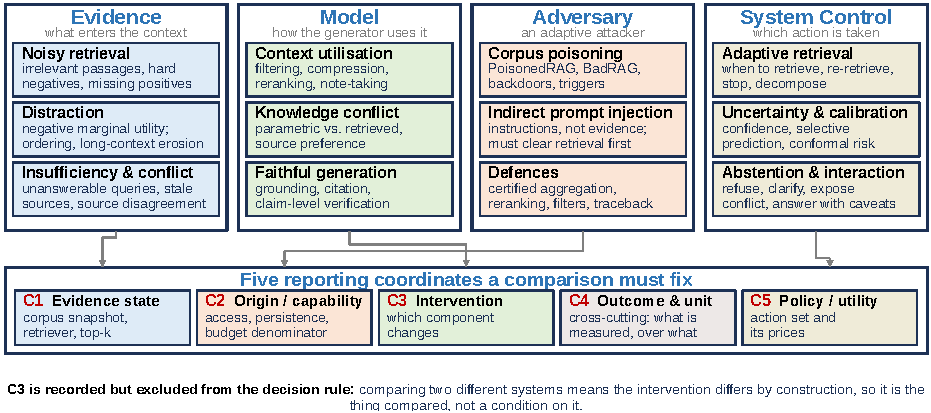
\includegraphics[width=\textwidth]{figures/generated/fig_taxonomy_map.pdf}%
\caption{The four failure surfaces and the reduction they support. Each column
is one surface of the survey (\S\ref{sec:evidence}--\S\ref{sec:system}); the
band below is the five reporting coordinates of \S\ref{sec:coordinates}, and the
connectors show which surface each coordinate collapses. C4 is cross-cutting
and has no single parent surface. The organisation is a partition of the
\emph{comparison} rather than of the literature: the columns tell a reader where
to look for related work, and the band tells a reader what must be stated on
both sides before two numbers can be placed together.}
\label{fig:hierarchical-taxonomy}
\end{figure*}

\begin{table*}[t]
\centering
\scriptsize
\renewcommand{\arraystretch}{0.88}
\begin{tabularx}{\linewidth}{>{\raggedright\arraybackslash}p{0.13\linewidth}>{\raggedright\arraybackslash}p{0.26\linewidth}>{\raggedright\arraybackslash}p{0.30\linewidth}X}
\toprule
\textbf{Coordinate} & \textbf{Controlled values} & \textbf{Equivalence / boundary rule} & \textbf{Verdict effect} \\
\midrule
Evidence state & Supported; irrelevant/distracting; insufficient; conflicting; stale/weak provenance; adversarially manipulated; not evidence-conditioned. & Code what is observable at the decision boundary. Query ambiguity, OOD input, confidence, and attacker access are not evidence states by themselves. & A direct performance claim normally requires a common state or an explicit cross-state estimand. \\
Origin / capability & Benign retrieval; constructed stressor; natural conflict/drift; query or distribution shift; attacker-created evidence; shared clean harness. & Record how the state arose. For security, include corpus write access, query control, retriever visibility, generator access, insertion budget, objective, and target. & A cross-source rank over two different games narrows at best and is otherwise undefined; a shared harness may deliberately vary capability as the controlled factor. \\
Intervention point & Corpus/index; retriever; reranker; context assembly/compression; generator prompting or training; verifier; system-control policy; evaluation-only artifact. & Code the component changed. Different interventions may be compared as alternatives when a shared end-to-end harness controls the remaining pipeline; otherwise they provide component-specific or compositional evidence. & C3 never enters the decision rule. Comparing two different systems means the intervention differs, so a C3 mismatch is the normal state of a comparison and cannot by itself make one undefined; it is recorded so a reader knows what changed. \\
Outcome / unit & Answer correctness; retrieval quality; evidence support; attack or defense utility; privacy leakage; calibration; selective risk/coverage; cost/latency; human preference. & Record definition, direction, aggregation, and unit. Relative gains over different baselines are not automatically a shared estimand. & A one-scalar ranking requires a common target. Without one there is no operating point to re-read at, so the gap is undefined rather than narrowed. \\
Policy / utility & Answer; abstain; re-retrieve; filter; verify; expose conflict; clarify; quarantine; recover; not applicable; unreported. & Use \emph{not applicable} for fixed descriptive comparisons. When policies compete, report action set, stakes, preferences, coverage, and cost. & Different actions can be ranked only under common utility; a signal alone does not establish the preferred response. A stated price at the other side's setting narrows the comparison. \\
Second-stage controls & Dataset/corpus snapshot; retriever/top-$k$/chunking; generator/decoding; compute budget; baselines; uncertainty/statistical design. & Select controls according to the stated inference. The tuple cannot remove confounding from unmatched experimental systems. & Tuple compatibility is necessary diagnostic information but not sufficient for a direct empirical ranking. \\
Final verdict & Survives; narrows; undefined. & Exactly the rule of \S\ref{sec:estimands}, and the only verdict vocabulary used anywhere in this paper or its artifacts. \emph{Survives}: C1, C2, C4 and C5 all match, so the quoted gap stands. \emph{Narrows}: a threatening coordinate differs but a side reports an operating point at the other's setting, or the comparison holds on a strict subset; report that matched number. \emph{Undefined}: no such operating point exists, or a decision-critical field is unavailable after full-text inspection. & Verdicts attach to comparison claims, not permanently to paper pairs, and a new shared-harness experiment can change the supported verdict. An undefined comparison is never replaced by a substitute number computed across the unmatched coordinate. \\
\bottomrule
\end{tabularx}
\caption{The decision procedure of \S\ref{sec:estimands} in full. The five coordinates diagnose semantic compatibility and claim-specific controls determine whether the claim as written is warranted, but only C1, C2, C4 and C5 enter the verdict: C3 is the thing being compared and is recorded rather than tested. The three verdicts here are the same three used in the body, the census codebook and every released artifact.}
\label{tab:framework-decision-procedure}
\end{table*}

\begin{table*}[t]
\centering
\scriptsize
\renewcommand{\arraystretch}{0.88}
\begin{tabularx}{\linewidth}{>{\raggedright\arraybackslash}p{0.18\linewidth}>{\raggedright\arraybackslash}p{0.31\linewidth}>{\raggedright\arraybackslash}p{0.25\linewidth}X}
\toprule
\textbf{Boundary case} & \textbf{Rule used in this paper} & \textbf{Verdict consequence} & \textbf{Example implication} \\
\midrule
Noisy retrieval vs. distraction & Retrieval imperfection alone is coded as relevance/noise; harmful influence on generation, confidence, or reasoning is coded as distraction. & Same broad topic but different measured effect is partial. & Random negatives and hard distractors should not be pooled into one score. \\
Query/OOD vs. evidence state & Query ambiguity, distribution shift, and model uncertainty describe the need or belief state. Code them under origin unless the study labels the resulting retrieved evidence. & Shared uncertainty language does not imply a common evidence state or policy. & An OOD detector is not automatically an insufficient-context detector. \\
Natural conflict vs. adversarial corruption & Code by the source of contradiction, not by surface form. Naturally occurring or diagnostic contradiction is conflict; attacker-created contradiction is integrity/adversarial corruption. & Natural-conflict and poisoning results are invalid as a direct ranking unless the threat model is redefined. & Faithfulness or source-preference methods are not poisoning defenses by default. \\
Intervention mismatch & Code the component changed, then inspect the evaluation harness. Different interventions can be compared as alternatives if the remaining pipeline and target are controlled. & Shared harness and end-to-end target can support valid comparison; unmatched pipelines support only a qualified comparison. & A filter and a note-taking prompt can be compared after fixing retriever, generator, evidence states, budget, and action utility. \\
Metric overlap & Metric targets must match the object being measured. Accuracy, citation support, attack success, calibration, and selective risk are separate families. & Shared dataset but different metric family is partial; mutually incompatible targets are invalid for one-scalar ranking. & A correct answer with unsupported citation should not pass a faithfulness comparison. \\
Observable but unnamed action & Infer behavior only when action is decision-relevant and the protocol is unambiguous; otherwise use \emph{not applicable}. & Merely omitting the phrase ``action policy'' does not force under-specification. & An answer-only benchmark supplies \emph{answer} for a policy claim, but a fixed latency comparison needs no action label. \\
Security capability missing & Mark only decision-critical missing access, budget, objective, or target as unknown. A shared harness may intentionally vary capability. & Unknown capability makes a cross-game rank under-specified; controlled capability variation can support a valid descriptive contrast. & Black- and white-box variants of one attack can be compared inside the same harness without implying cross-paper transfer. \\
Benchmark vs. method & Code benchmark if the reusable artifact is the main contribution; otherwise code the intervention. & Benchmark-method comparison is partial unless the method is evaluated on the benchmark under aligned assumptions. & RGB is benchmark-first; RAAT is training-first. \\
Tuple match but control mismatch & After semantic coding, inspect corpus, data, retriever, generator, top-$k$, budget, baselines, decoding, and uncertainty. & A tuple match is insufficient for direct ranking when these factors confound the reported score. & Two answer-only noise methods on different datasets and generators require a shared rerun or a qualified claim. \\
\bottomrule
\end{tabularx}
\caption{Boundary rules for applying the revised diagnostic schema. Verdicts are claim-specific and require both semantic and experimental-control checks.}
\label{tab:taxonomy-rules}
\end{table*}

\begin{table*}[t]
\centering
\small
\begin{tabularx}{\linewidth}{p{0.14\linewidth}p{0.2\linewidth}p{0.27\linewidth}X}
\toprule
\textbf{Stage} & \textbf{Question} & \textbf{Typical signals} & \textbf{Representative actions} \\
\midrule
Detect & Is the current evidence unreliable? & Low retrieval confidence, high contradiction, low sufficient-context score, suspicious document patterns & Flag query/evidence, route to stronger checks, log risk state \\
Diagnose & What kind of unreliability is present? & Irrelevance, distraction, conflict, poisoning, ambiguity, unanswerability, stale evidence & Assign failure type; separate benign noise from adversarial risk \\
Mitigate & Can the evidence be repaired before answering? & Alternative retrieval results, filter scores, reranker utility, provenance, source agreement & Re-rank, filter, compress, re-query, retrieve from trusted sources, remove malicious passages \\
Control & What should the system do now? & Calibrated confidence, selective risk, cost budget, user risk tolerance & Answer, abstain, ask clarification, expose conflict, escalate to human review \\
Monitor & Did the system fail or get attacked? & User feedback, traceback signals, poisoned-document clusters, drift over time & Update index, quarantine sources, revise prompts, retrain filters, update audit logs \\
\bottomrule
\end{tabularx}
\caption{An operational pipeline for robust RAG. The pipeline turns the paper's taxonomy into actionable system design steps.}
\label{tab:operational-pipeline}
\end{table*}

\begin{figure*}[t]
\centering
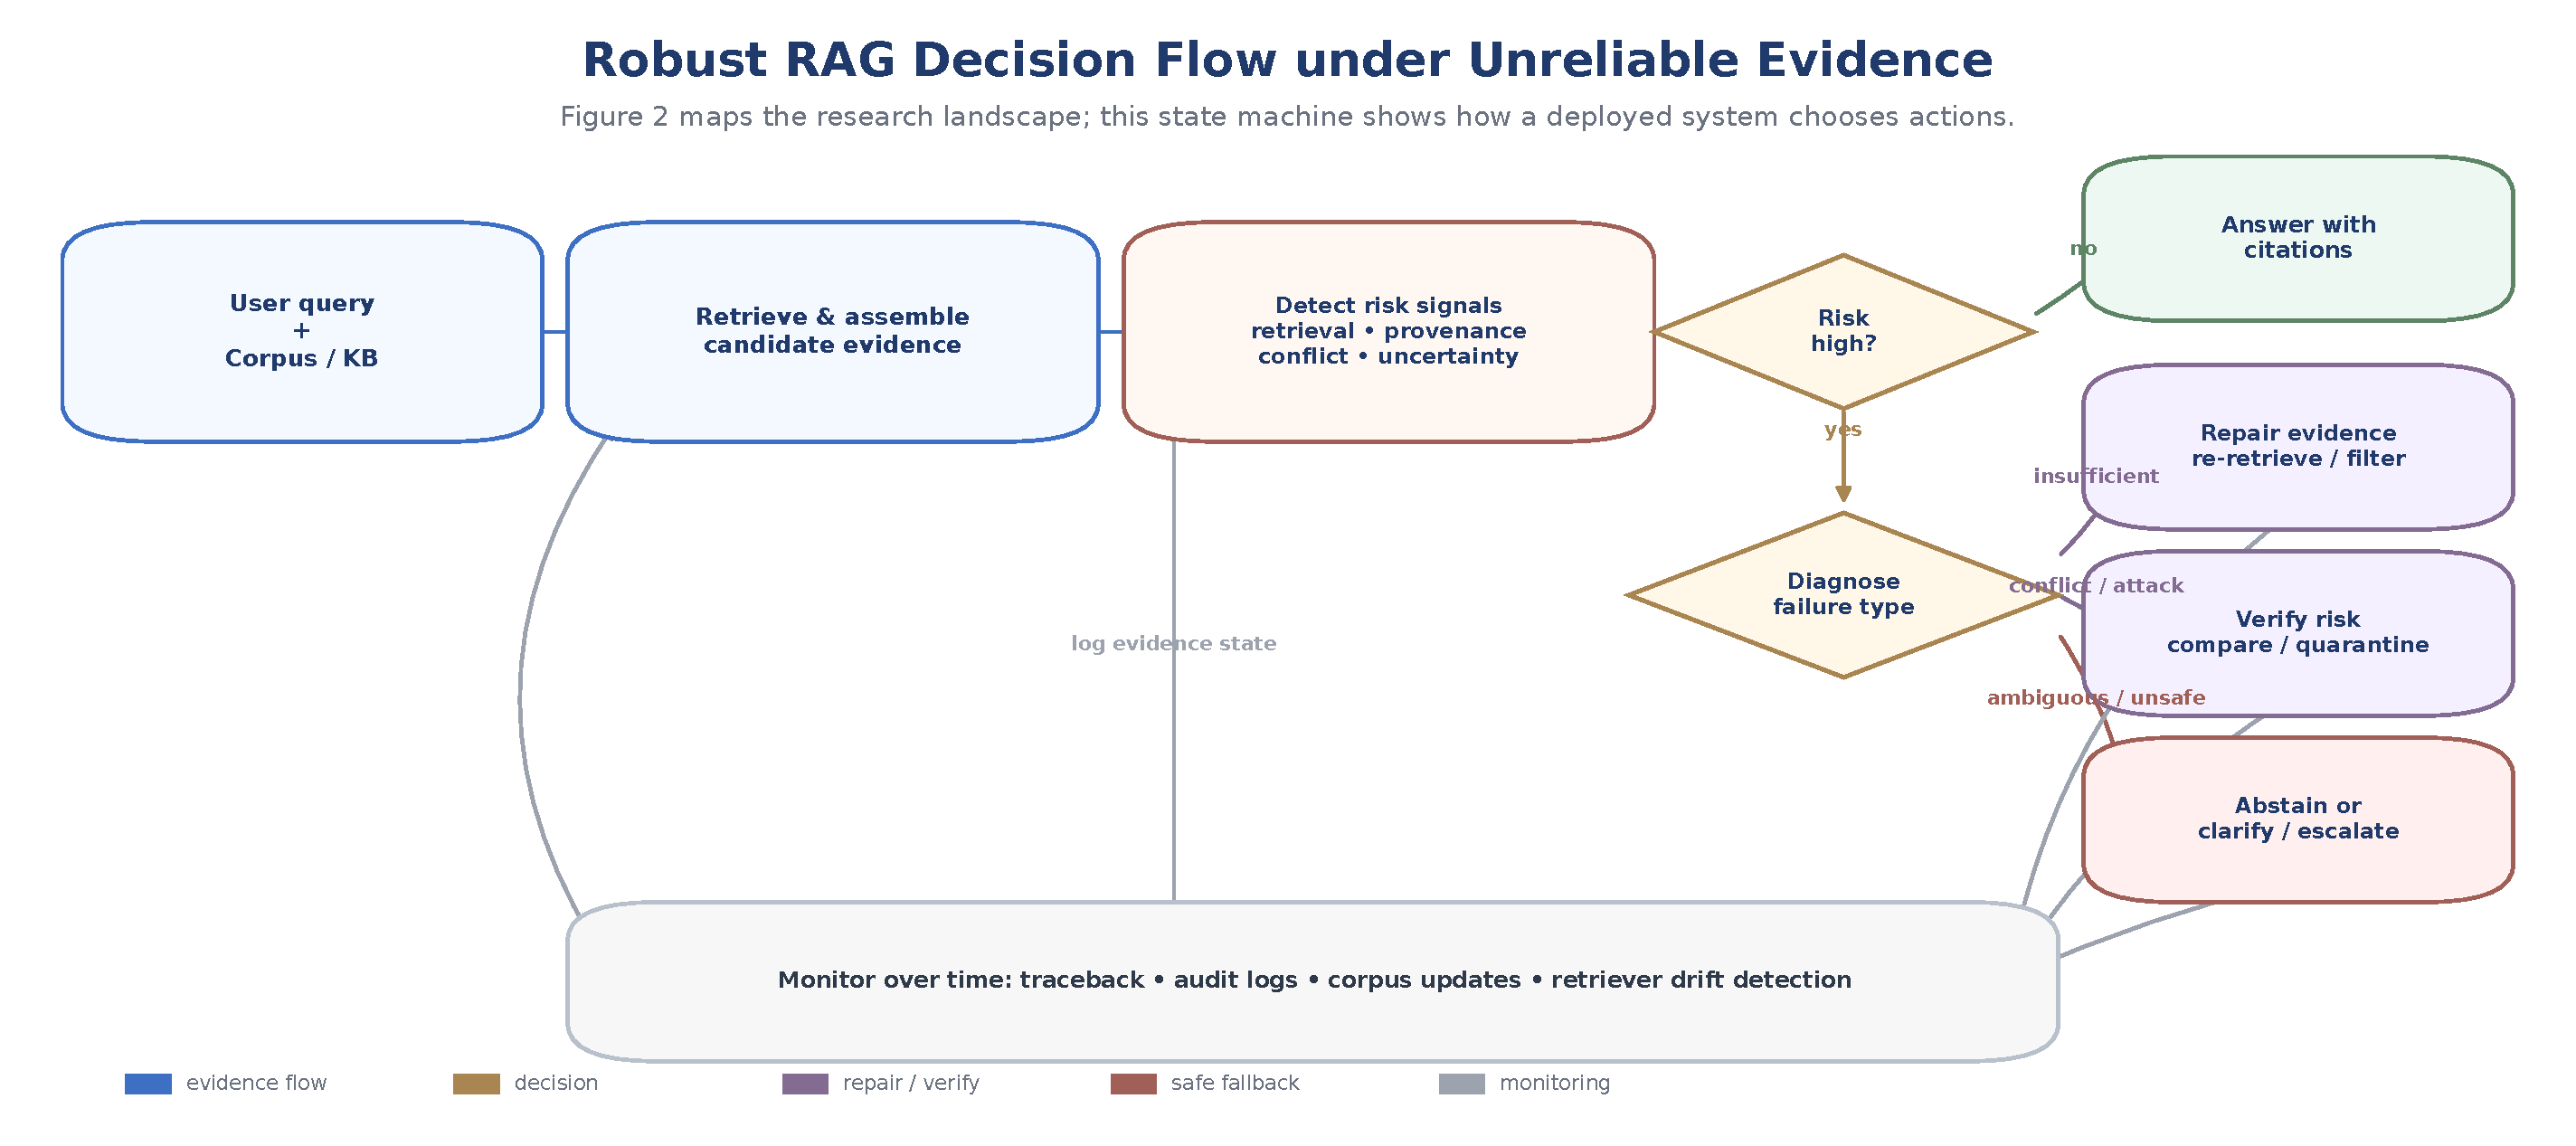
\includegraphics[width=\textwidth,keepaspectratio]{figures/generated/fig3_operational_decision_flow_py_4k.pdf}
\caption{Operational decision flow for robust RAG. Unlike the taxonomy in Figure~\ref{fig:hierarchical-taxonomy}, this state-machine view describes the branching actions a deployed system can take when unreliable evidence is encountered: answer, repair evidence, verify risk, abstain, clarify, escalate, or monitor.}
\label{fig:operational-pipeline-image}
\end{figure*}

\begin{table*}[t]
\centering
\small
\begin{tabularx}{\linewidth}{p{0.18\linewidth}p{0.18\linewidth}p{0.25\linewidth}X}
\toprule
\textbf{Theme} & \textbf{Representative work} & \textbf{Core idea} & \textbf{What it reveals for robust RAG} \\
\midrule
Irrelevant context & \citetalias{irrelevantContext2023} & Analyze and mitigate irrelevant retrieved context with filtering and robust training & Even answerable questions degrade when irrelevant passages enter the context; robustness is not equivalent to retrieval recall. \\
Retrieval-noise training & \citetalias{raat2024} & Categorize retrieval noise and train with adaptive adversarial objectives & Noise types should be separated: irrelevant, relevant-but-insufficient, and counterfactual evidence have different effects. \\
Generator note-taking & \citetalias{chainOfNote2023} & Generate per-passage notes before answering & Robust generation benefits from intermediate relevance judgments rather than direct answer generation. \\
Fine-grained noise benchmark & \citetalias{rrag027} & Configurable benchmark for distracting, low-quality, inconsequential, and irrelevant noise & ``Noise'' is not monolithic; evaluation should vary type, amount, and placement of bad evidence. \\
Nonlinear distraction & \citetalias{rrag003} & Study disproportionate effect of small amounts of misleading information & A few strong distractors can dominate long-context reasoning, so average noise rate is insufficient. \\
Long-context RAG & \citetalias{rrag039} & Analyze long-input RAG and hard negatives & More retrieved context can hurt unless ordering, filtering, or training adapts to long-context failure modes. \\
Sentence-level filtering & \citetalias{rrag044} & Filter retrieved context before generation & Filtering can be more fine-grained than document reranking and can remove local distractors inside otherwise useful passages. \\
Retrieval evaluation & \citetalias{rrag058} & Utility-aware retrieval metric for LLMs & RAG retrieval should be evaluated by downstream utility, including negative utility from distracting passages. \\
\bottomrule
\end{tabularx}
\caption{Representative evidence-centric work on noisy retrieval and distraction.}
\label{tab:evidence-methods}
\end{table*}

\begin{table*}[t]
\centering
\small
\begin{tabularx}{\linewidth}{p{0.2\linewidth}p{0.2\linewidth}p{0.28\linewidth}X}
\toprule
\textbf{Problem} & \textbf{Representative work} & \textbf{Mechanism} & \textbf{Limitation or open issue} \\
\midrule
Parametric--retrieved conflict & \citetalias{tugOfWar2024} & Construct and analyze conflicts between internal and external knowledge & Conflict behavior depends on model, prompt, evidence coherence, and task framing. \\
Fact-level conflict modeling & \citetalias{faithfulRAG2025} & Extract parametric self-facts, align them with retrieved facts, and reason before answering & Requires reliable fact extraction and alignment; complex claims remain difficult. \\
Source-aware consolidation & \citetalias{astuteRAG2025} & Elicit internal knowledge and consolidate it with retrieved sources using reliability comparison & Training-free but still depends on LLM self-assessment and source-quality cues. \\
Hidden-state rectification & \citetalias{rrag008} & Locate layers where parametric suppression occurs and contrast contextual/non-contextual logits & Promising for model-centric control, but model internals and transferability remain open. \\
Context utilisation benchmarks & \citetalias{rrag032} & Test gold, conflicting, and irrelevant contexts across models & Benchmarks reveal whether a model uses context, but not always why a model chooses one source. \\
Real-document conflict & \citetalias{rrag112} & Study behavior under context-memory conflicts with real documents & Realistic evidence can be messier than synthetic conflicts and harder to label. \\
Source preference & \citetalias{rrag132} & Analyze which sources win under conflict & Source preference may encode bias, recency effects, or authority priors. \\
\bottomrule
\end{tabularx}
\caption{Representative model-centric work on knowledge conflict and contextual faithfulness.}
\label{tab:conflict-methods}
\end{table*}

\begin{table*}[t]
\centering
\small
\begin{tabularx}{\linewidth}{p{0.17\linewidth}p{0.19\linewidth}p{0.25\linewidth}X}
\toprule
\textbf{Attack/defense surface} & \textbf{Representative work} & \textbf{Threat or defense} & \textbf{Implication} \\
\midrule
Retriever poisoning & \citetalias{poisoningRetrievalCorpora2023} & Inject adversarial passages to manipulate dense retrievers & Retrieval security can fail before generation begins. \\
RAG knowledge corruption & \citetalias{poisonedRAG2024} & Craft malicious passages that steer generated answers & End-to-end RAG needs corpus integrity and generation safeguards. \\
Backdoor attacks & \citetalias{trojanRAG2024}; \citetalias{phantom2024} & Triggered retrieval/generation behavior via poisoned contexts & RAG can act as a backdoor carrier without modifying model weights. \\
Prompt template attacks & \citetalias{aip2025} & Weaponize shared instructional prompts to steer retrieval and generation & Prompt templates are part of the attack surface, not just implementation details. \\
Indirect prompt injection & \citetalias{rrag005} & Optimize trigger fragments so malicious instructions are retrieved in the wild & Real attacks must overcome the retrieval barrier, not merely place malicious text in a corpus. \\
Certified defense & \citetalias{certifiedRAG2024} & Isolate-and-aggregate answers for robustness certificates & Certification gives stronger guarantees but typically assumes specific attack budgets. \\
Reranking defense & \citetalias{rrag004} & Use probe-gradient instability to demote poisoned passages & Defense can be inserted retriever-side without retraining the LLM. \\
Attention defense & \citetalias{rrag015} & Detect poisoning via normalised attention variance & Internal attention signals may expose poisoned evidence, but adaptivity remains a concern. \\
\bottomrule
\end{tabularx}
\caption{Representative adversarial corruption attacks and defenses.}
\label{tab:adversarial-methods}
\end{table*}

\begin{table*}[t]
\centering
\scriptsize
\renewcommand{\arraystretch}{0.88}
\begin{tabularx}{\linewidth}{>{\raggedright\arraybackslash}p{0.18\linewidth}c c c c >{\raggedright\arraybackslash}p{0.15\linewidth}X}
\toprule
\textbf{Threat class} & \textbf{Corpus} & \textbf{Query} & \textbf{Retr.} & \textbf{Gen.} & \textbf{Objective} & \textbf{Boundary} \\
\midrule
Dense-retriever poisoning \citep{poisoningRetrievalCorpora2023} & write & train set & white/gray & no & retrieve bad passages & Not always end-to-end. \\
RAG knowledge corruption \citep{poisonedRAG2024,badRAG2024} & write & target topic & black/gray & black & answer steering & Stealth/dynamics vary. \\
Backdoor-style RAG \citep{trojanRAG2024,phantom2024} & write & trigger & gray & black & latent behavior & Normal queries may pass. \\
Indirect prompt injection \citep{aip2025,rrag005} & write/share & natural & black & black & instruction hijack & Must overcome retrieval. \\
Opinion/fairness manipulation \citep{rrag104,rrag162} & write & group/topic & black/gray & black & bias steering & QA metrics miss social harm. \\
Defense setting \citep{certifiedRAG2024,rrag004,rrag015,rrag128} & bounded & varies & assumed & black/gray & detect/demote/trace & Depends on budget/visibility. \\
\bottomrule
\end{tabularx}
\caption{Attacker-capability matrix for adversarial RAG. The same ``attack success rate'' can mean different things depending on corpus write access, query control, retriever visibility, generator access, and objective.}
\label{tab:attacker-capability}
\end{table*}

\begin{table*}[t]
\centering
\scriptsize
\renewcommand{\arraystretch}{0.88}
\begin{tabularx}{\linewidth}{>{\raggedright\arraybackslash}p{0.17\linewidth}>{\raggedright\arraybackslash}p{0.21\linewidth}>{\raggedright\arraybackslash}p{0.22\linewidth}>{\raggedright\arraybackslash}p{0.16\linewidth}X}
\toprule
\textbf{Comparison} & \textbf{Why it looks comparable} & \textbf{Hidden mismatch} & \textbf{Metric pitfall} & \textbf{Normalised reading} \\
\midrule
PoisonedRAG vs. dense-retriever poisoning & Both insert malicious evidence into a retrieval corpus. & One evaluates end-to-end answer steering; the other may evaluate retriever ranking before generation. & Retrieval success and answer attack success are not the same target. & Compare only after recording whether poisoned evidence is retrieved and whether the generator changes the final answer. \\
Certified RAG defense vs. prompt-injection defense & Both are RAG defenses against corrupted retrieved content. & Certification assumes a bounded number of corrupted passages; prompt injection exploits instruction following rather than only false facts. & A certificate under bounded corruption may not imply instruction-hijack resistance. & Treat certification, instruction isolation, and document sanitisation as complementary defenses. \\
Traceback vs. prevention & Both reduce harm after poisoning. & Traceback identifies influential poisoned documents after failure; prevention attempts to block harmful output before response. & Lower post-hoc traceback error does not equal lower user-facing attack success. & Report prevention, detection, demotion, traceback, and recovery as separate outcome variables. \\
Backdoor trigger vs. natural query attack & Both can produce targeted malicious behavior. & Trigger attacks may rely on rare phrases; natural-query attacks must survive ordinary retrieval and ranking. & Attack success under attacker-crafted triggers overstates risk under natural user queries. & Require query-control and trigger-frequency fields before comparing attack strength. \\
\bottomrule
\end{tabularx}
\caption{Concrete examples of threat-model normalisation. These cases show how reported attack or defense success can reverse when attacker access, retrieval realism, and evaluation target differ.}
\label{tab:threat-model-examples}
\end{table*}


\begin{table*}[t]
\centering
\small
\begin{tabularx}{\linewidth}{p{0.16\linewidth}p{0.18\linewidth}p{0.28\linewidth}X}
\toprule
\textbf{Control/evaluation question} & \textbf{Representative work} & \textbf{Signal or decision} & \textbf{Why it matters} \\
\midrule
When to retrieve & \citetalias{selfRAG2023}; \citetalias{whenToRetrieve2024}; \citetalias{ctrla2025} & Reflection tokens, special retrieval tokens, or representation-based confidence/honesty directions & Retrieval is an action with costs and risks, not a fixed preprocessing step. \\
When retrieval is weak & \citetalias{crag2024}; \citetalias{sufficientContext2024} & Retrieval evaluator or sufficient-context signal & A system should repair or abstain rather than answer from insufficient evidence. \\
Calibration & \citetalias{calibRAG2025}; \citetalias{uncertaintyRAG2024}; \citetalias{rrag007} & Decision calibration, span uncertainty, verbal confidence calibration & Robustness requires confidence to reflect both model and evidence uncertainty. \\
Unanswerability & \citetalias{rrag111}; \citetalias{rrag141} & Unanswerable and underspecified RAG benchmarks & Real users often ask questions the corpus cannot answer; refusal and clarification need direct evaluation. \\
RAG capabilities & \citetalias{rgb2023} & Noise robustness, negative rejection, integration, counterfactual robustness & Multi-axis evaluation exposes failures hidden by answer accuracy. \\
Hallucination detection & \citetalias{ragTruth2024} & Word-level hallucination annotations for RAG outputs & Fine-grained labels support detection and attribution beyond answer-level scoring. \\
Query robustness & \citetalias{queryRobustness2025} & Perturb query wording and measure pipeline sensitivity & Robustness must include the query-to-retrieval interface. \\
\bottomrule
\end{tabularx}
\caption{Representative work on system-centric control and evaluation.}
\label{tab:control-eval-methods}
\end{table*}

\begin{table*}[t]
\centering
\scriptsize
\renewcommand{\arraystretch}{0.9}
\begin{tabularx}{\linewidth}{>{\raggedright\arraybackslash}p{0.18\linewidth}>{\raggedright\arraybackslash}p{0.22\linewidth}>{\raggedright\arraybackslash}p{0.25\linewidth}X}
\toprule
\textbf{Lineage} & \textbf{Classical question} & \textbf{RAG-specific version} & \textbf{Why it matters for robust RAG} \\
\midrule
Selective prediction & When should a model abstain to control risk? & Abstain when retrieved evidence is insufficient, conflicting, stale, or corrupted. & Selective risk must condition on evidence state, not only answer confidence. \\
Calibration & Does confidence match correctness? & Does confidence match answer correctness, evidence sufficiency, citation support, and retrieval usefulness? & A calibrated answer probability can still hide unreliable evidence. \\
Active clarification & When should the system ask a user for more information? & Ask clarification before retrieval when the query is ambiguous or underspecified. & Clarification can be the correct action even when retrieval could produce a plausible answer. \\
Cost-sensitive retrieval & When is additional computation worth it? & Decide whether to retrieve, re-retrieve, verify, rerank, or escalate under latency/cost budgets. & Robustness gains should be reported with action cost and coverage, not only accuracy. \\
Decision-theoretic control & Which action minimizes expected risk? & Choose among answer, abstain, expose conflict, cite uncertainty, retrieve again, or quarantine evidence. & Action quality is the bridge between evidence reliability estimates and user-facing behavior. \\
\bottomrule
\end{tabularx}
\caption{Action-control lineage. The framework imports ideas from selective prediction, calibration, clarification, and cost-sensitive decision-making, but makes retrieved evidence state the object being controlled.}
\label{tab:action-control-lineage}
\end{table*}



\section{Evaluation Details}
\label{sec:appendix-eval}
% Drawn by scripts/revision3/fig_appendix_schematics.py; the .pptx is the
% editable source and is released with the paper.
\begin{figure*}[t]
\centering
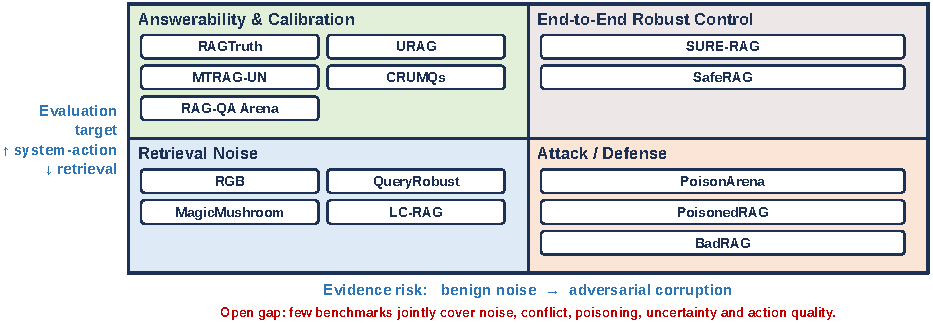
\includegraphics[width=\textwidth]{figures/generated/fig_benchmark_landscape.pdf}%
\caption{Conceptual benchmark landscape. Placement is illustrative rather than
data-derived; the figure organises differences in evidence risk and evaluation
level, not empirical distance or benchmark quality. The two axes are
coordinates C1 and C4, and the open gap is the reason a single ``robustness''
number rarely transfers between quadrants.}
\label{fig:benchmark-landscape}
\end{figure*}

\begin{table*}[t]
\centering
\scriptsize
\renewcommand{\arraystretch}{0.95}
\begin{tabularx}{\linewidth}{>{\raggedright\arraybackslash}p{0.12\linewidth}>{\raggedright\arraybackslash}p{0.13\linewidth}>{\raggedright\arraybackslash}p{0.17\linewidth}>{\raggedright\arraybackslash}p{0.18\linewidth}>{\raggedright\arraybackslash}p{0.14\linewidth}X}
\toprule
\textbf{Benchmark} & \textbf{Risk focus} & \textbf{Task / data} & \textbf{Perturbation or threat} & \textbf{Metrics} & \textbf{Boundary} \\
\midrule
RGB \citep{rgb2023} & noise, rejection, integration, counterfactuality & English/Chinese QA & noisy passages, false evidence, negative evidence & accuracy, ability-specific scores & Broad diagnostic benchmark but not adaptive attack-oriented. \\
RAGTruth \citep{ragTruth2024} & hallucination / faithfulness & QA, data-to-text, summarization & naturally generated unsupported spans & word-level hallucination labels & Strong annotation granularity; less focused on retrieval-side threat models. \\
Sufficient Context \citep{sufficientContext2024} & answerability & QA with context sufficiency labels & insufficient retrieved evidence & selective generation / abstention & Captures answerability but not adversarial corruption. \\
MagicMushroom \citep{rrag027} & retrieval noise & configurable RAG stress tests & distracting, low-quality, inconsequential, irrelevant noise & robustness under noise types & Fine-grained noise; limited conflict/security coverage. \\
URAG \citep{rrag001} & uncertainty & RAG as MCQA / conformal prediction & irrelevant/noisy retrieval and uncertainty sets & coverage, set size, calibration & Good for uncertainty; less direct for free-form generation. \\
QueryRobust \citep{queryRobustness2025} & query robustness & QA with query perturbations & wording variation at query--retrieval interface & retrieval and end-task degradation & Focuses on query perturbation, not corpus corruption. \\
PoisonArena \citep{rrag023} & adversarial poisoning & RAG attack competition setting & competing poisoning attacks & attack success, retrieval effects & Strong security focus; benign uncertainty is secondary. \\
SafeRAG \citep{rrag019} & RAG security & security benchmark for RAG & poisoning / malicious retrieval contexts & attack and defense metrics & Security-oriented; not a full evidence reliability suite. \\
MTRAG-UN \citep{rrag141} & multi-turn unanswerability & multi-turn RAG conversations & unanswerable, underspecified, non-standalone questions & abstention / clarification quality & Covers interaction; less focused on adversarial evidence. \\
CRUMQs \citep{rrag193} & unanswerable multi-hop RAG & realistic multi-hop queries & unanswerable and uncheatable questions & answerability and robustness & Useful for abstention; not a broad attack/noise benchmark. \\
\bottomrule
\end{tabularx}
\caption{Benchmark-level comparison for robust RAG evaluation. The table makes explicit what each benchmark perturbs, what it measures, and which failure modes remain outside its scope.}
\label{tab:benchmark-comparison}
\end{table*}


\begin{table*}[t]
\centering
\scriptsize
\begin{tabularx}{\linewidth}{p{0.18\linewidth}p{0.22\linewidth}p{0.24\linewidth}X}
\toprule
\textbf{Benchmark component} & \textbf{Required annotation} & \textbf{Metric suite} & \textbf{Why it is needed} \\
\midrule
Evidence reliability & relevance, sufficiency, freshness, provenance, support span & retrieval recall, sufficient-context accuracy, support precision & Distinguishes merely related passages from answer-supporting evidence. \\
Distraction and conflict & distractor type, conflicting claim pair, source agreement & answer flip rate, conflict sensitivity, context-utilisation score & Reveals whether models ignore harmful context or silently pick a source. \\
Adversarial corruption & attacker access, insertion budget, trigger type, poisoned document ID & attack success, poisoned retrieval rate, stealth, defense bypass & Makes security results comparable across threat models. \\
Unanswerability and ambiguity & answerability label, ambiguity type, clarification target & selective risk, abstention precision/recall, clarification accuracy & Evaluates robust action selection, not just answer generation. \\
Cost and system action & number of retrievals, verifier calls, latency, final action trace & cost-adjusted accuracy, action utility, coverage--risk curve & Prevents methods from hiding robustness gains behind unbounded computation. \\
\bottomrule
\end{tabularx}
\caption{A proposed benchmark blueprint for robust RAG under unreliable evidence. This is a research agenda rather than a validated leaderboard; existing benchmarks cover parts of the schema.}
\label{tab:benchmark-blueprint}
\end{table*}

\begin{table*}[t]
\centering
\tiny
\renewcommand{\arraystretch}{0.88}
\begin{tabularx}{\linewidth}{>{\raggedright\arraybackslash}p{0.16\linewidth}>{\raggedright\arraybackslash}p{0.19\linewidth}>{\raggedright\arraybackslash}p{0.17\linewidth}>{\raggedright\arraybackslash}p{0.16\linewidth}X}
\toprule
\textbf{Example query} & \textbf{Retrieved evidence state} & \textbf{Correct action} & \textbf{Wrong action} & \textbf{Metric consequence} \\
\midrule
``What is the refund deadline in policy version 3?'' & Gold policy passage is present, but a high-ranked older policy gives a different deadline. & Compare provenance/date, prefer the current policy, cite the supporting span. & Answer from the older top-ranked passage. & Answer accuracy alone may mark one string right/wrong; action-aware scoring credits source freshness and conflict handling. \\
``Which paper introduced method X's ablation result?'' & Retrieved documents are topically related but none contains the requested ablation. & Detect insufficiency and re-retrieve or abstain with missing-evidence explanation. & Guess from a related abstract. & Selective risk and sufficiency detection should be rewarded; forced-answer accuracy should not. \\
``Summarize whether product Y is safe for use case Z.'' & Retrieved reviews contain plausible positive statements and a contradictory safety notice from an authoritative source. & Expose conflict, prioritize authoritative safety evidence, or escalate. & Produce a balanced answer that hides the conflict. & Faithfulness to a retrieved passage is not enough; metric must score conflict disclosure and source authority. \\
``What does the linked document instruct the assistant to do?'' & A retrieved document contains task-irrelevant instructions mixed with factual content. & Treat instructions as untrusted evidence, filter or quarantine, then answer only from factual support. & Follow the retrieved instruction. & Attack success must be separated from poisoned retrieval and from final answer utility. \\
``Should the system answer now or search again?'' & Current evidence is relevant but incomplete; a second retrieval is available at latency cost. & Choose re-retrieval if expected utility exceeds cost, otherwise abstain. & Answer immediately with overconfident unsupported text. & Calibration error alone is insufficient; score action utility, coverage, latency, and evidence sufficiency. \\
\bottomrule
\end{tabularx}
\caption{Illustrative action-labeled evaluation blueprint. Rows are examples of the annotation schema implied by the re-analyses, not a released benchmark or empirical leaderboard.}
\label{tab:action-labeled-blueprint-examples}
\end{table*}


\begin{table}[t]
\centering
\scriptsize
\begin{tabular}{lrrrr}
\toprule
\textbf{Policy} & \textbf{Ans.} & \textbf{Act.} & \textbf{Joint} & \textbf{Unsafe} \\
\midrule
Answer-only & 0.17 & 0.17 & 0.17 & 0.83 \\
Abstain-on-missing & 0.67 & 0.33 & 0.33 & 0.17 \\
Zero-shot LLM & 0.83 & 0.83 & 0.83 & 0.00 \\
State-label heuristic & 1.00 & 1.00 & 1.00 & 0.00 \\
\bottomrule
\end{tabular}
\caption{Minimal action-labeled pilot over 60 diagnostic items. \emph{Zero-shot LLM} is GPT-4o and Claude Sonnet-4.6 (identical here), each given the query and retrieved-evidence situation but not the gold action; both select the correct action on 50/60 items and never answer when they should withhold, their only misses choosing \emph{filter} over the gold top-level \emph{answer} on noise items. The \emph{state-label heuristic} reads the gold evidence-state label and is an upper-bound sanity check, not a deployed model. Unsafe is the rate of answering when the gold action is to abstain, quarantine, clarify, expose conflict, or re-retrieve.}
\label{tab:action-labeled-pilot-results}
\end{table}


\begin{table*}[t]
\centering
\scriptsize
\renewcommand{\arraystretch}{0.92}
\begin{tabularx}{\linewidth}{>{\raggedright\arraybackslash}p{0.17\linewidth}>{\raggedright\arraybackslash}p{0.27\linewidth}>{\raggedright\arraybackslash}p{0.25\linewidth}X}
\toprule
\textbf{Axis} & \textbf{Typical variation across papers} & \textbf{Why conclusions fail to transfer} & \textbf{Minimum reporting requirement} \\
\midrule
Retriever/generator setting & BM25 vs dense vs hybrid retrieval; small vs frontier generators; frozen vs fine-tuned models & A defense may work by compensating for one retriever or one model scale rather than solving the failure mode. & Retriever, index, top-$k$, reranker, generator, prompt, decoding, and context length. \\
Attack budget and access & Poisoned-document count, corpus write access, query control, retriever visibility, generator access & Attack success rates are incomparable when one attacker edits a corpus and another only controls the query. & Capability matrix, insertion budget, target set, stealth objective, and whether malicious evidence is retrieved. \\
Metric target & EM/F1, faithfulness, citation support, attack success, calibration error, selective risk, cost & Improving answer accuracy can worsen citation faithfulness; improving abstention can reduce coverage; reducing attacks can lower utility. & Report utility, evidence support, risk, calibration, cost, and security as a Pareto surface. \\
Statistical and reproducibility evidence & Single seed/model vs multiple seeds/models; code/data availability varies & Small prompt or model changes can reverse robustness rankings, especially for LLM-as-judge or attack benchmarks. & Seeds, confidence intervals or bootstrap tests where feasible, released prompts, data splits, and code or exact API settings. \\
Long-context baseline & RAG-only comparisons vs long-context LLMs with the same documents & A robustness gain may reflect retrieval compression rather than evidence reliability control. & Include a long-context or full-context baseline when context length permits, and report latency/cost. \\
Attribution vs answer accuracy & Some tasks score only final answer; others require evidence-supported citations & A model can answer correctly for the wrong reason, cite irrelevant evidence, or ignore retrieved support. & Claim-level support labels, citation precision/recall, and answer correctness reported separately. \\
\bottomrule
\end{tabularx}
\caption{Evaluation-assumption matrix for robust RAG. The table summarises why benchmark results often cannot be compared without aligning system setup, threat model, metric target, reproducibility evidence, and long-context baselines.}
\label{tab:evaluation-assumption-matrix}
\end{table*}


% Drawn by scripts/revision3/fig_appendix_schematics.py; the .pptx is the
% editable source and is released with the paper.
\begin{figure*}[t]
\centering
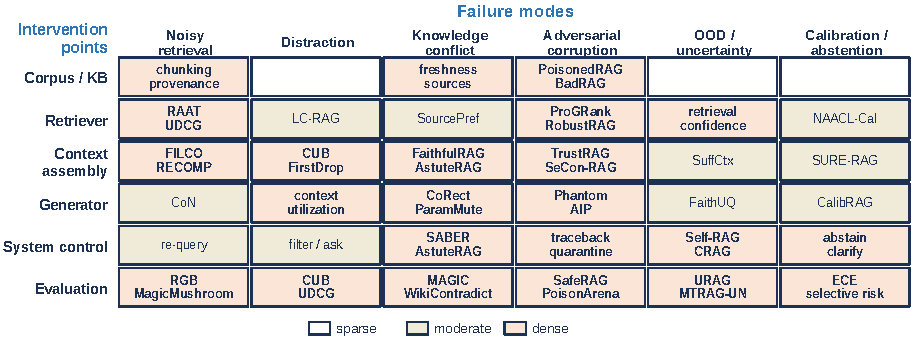
\includegraphics[width=\textwidth]{figures/generated/fig_failure_matrix.pdf}%
\caption{Schematic literature-family $\times$ intervention matrix. Shading and
example labels are illustrative design aids, not counts from Map~B;
quantitative Map-B distributions appear in Table~\ref{tab:corpus-stats}. Rows
are coordinate C3 and columns are coordinate C1, which is why a cell, not a
column, is the unit at which two systems become comparable.}
\label{fig:failure-intervention-matrix}
\end{figure*}

\begin{table*}[t]
\centering
\scriptsize
\renewcommand{\arraystretch}{0.92}
\begin{tabularx}{\linewidth}{>{\raggedright\arraybackslash}p{0.13\linewidth}>{\raggedright\arraybackslash}p{0.12\linewidth}>{\raggedright\arraybackslash}p{0.16\linewidth}>{\raggedright\arraybackslash}p{0.18\linewidth}>{\raggedright\arraybackslash}p{0.13\linewidth}>{\raggedright\arraybackslash}X}
\toprule
\textbf{Work} & \textbf{Failure} & \textbf{Task / setup} & \textbf{Key assumption} & \textbf{Metric} & \textbf{Boundary} \\
\midrule
IrrelCtx & irrelevant context & Open-domain QA & Irrelevance can be filtered or learned against & Robust accuracy & No adversarial/conflict setting. \\
RAAT & retrieval noise & Noisy QA training & Noise-aware training improves generation & F1/EM & Needs deployment-like noise. \\
RGB & multi-ability RAG & Bilingual benchmark & RAG reliability decomposes into abilities & Ability accuracy & Not adversarially adaptive. \\
FaithfulRAG & conflict & Fact-level conflict & Conflicts can be localised and reasoned over & Faithfulness & Needs reliable fact extraction. \\
AstuteRAG & imperfect retrieval & Training-free consolidation & Internal/external knowledge can be reliability-compared & Robust QA & Depends on LLM self-assessment. \\
PoisonedRAG & poisoning & Injected passages & Few crafted passages can dominate retrieval & Attack success & Targeted corruption focus. \\
RobustRAG & defense & Bounded corruption & Isolate-and-aggregate can certify robustness & Certificate, accuracy & Assumes attack budget. \\
Self-RAG / CtrlA & adaptive retrieval & Retrieve-or-answer & Model state can trigger retrieval & Trigger quality & Calibration can shift. \\
CalibRAG / URAG & calibration & Decision/MCQA & Confidence should reflect evidence uncertainty & ECE, coverage & Does not repair evidence. \\
PoisonArena / SafeRAG & security eval. & Poisoning benchmark & Threat models must be explicit & ASR, bypass & Still isolates attacks. \\
\bottomrule
\end{tabularx}
\caption{Analytical matrix of representative robust RAG work. Compared with a citation list, the matrix highlights each work's task setup, central assumption, metric focus, and boundary of applicability.}
\label{tab:analytical-matrix}
\end{table*}

\begin{table*}[t]
\centering
\scriptsize
\renewcommand{\arraystretch}{0.86}
\begin{tabularx}{\linewidth}{>{\raggedright\arraybackslash}p{0.14\linewidth}>{\raggedright\arraybackslash}p{0.19\linewidth}>{\raggedright\arraybackslash}p{0.24\linewidth}>{\raggedright\arraybackslash}p{0.18\linewidth}X}
\toprule
\textbf{Case} & \textbf{Released rows / papers} & \textbf{Audited comparison fields} & \textbf{Metric or failure conflict} & \textbf{Synthesis / artifact boundary} \\
\midrule
Noise / distraction robustness & 5 rows: IrrelCtx, RAAT, Chain-of-Note, Sufficient Context, RGB & Assumption, QA dataset or benchmark slice, generator / reader setup, negative type, rank and gold-evidence availability. & EM/F1, rejection, selective risk, and ability-specific benchmark scores answer different questions. & Treat filtering, noise-aware training, generator reading, sufficiency prediction, and benchmark diagnosis as different mechanisms; artifact status is recorded per paper in the released worksheet. \\
Faithfulness, conflict, and attribution & 5 rows: RAGTruth, FaithfulRAG, AstuteRAG, Tug-of-War, Chain-of-Note & Unit of support, source-conflict assumption, attribution granularity, model-side reasoning setup, artifact availability. & Span-level support, fact-level conflict resolution, source preference, and final answer accuracy can disagree. & Citation faithfulness should not be collapsed into conflict robustness; the worksheet records where artifact evidence is dataset-level, code-level, or paper-only. \\
Adversarial corruption and RAG security & 6 rows: PoisonedRAG, corpus poisoning, BadRAG, certified defense, TrojanRAG, traceback & Corpus write access, insertion budget, retriever visibility, query control, generator access, stealth, retrieved malicious evidence, defense timing. & Attack success, certified robust accuracy, detection, traceback, and clean utility are not one defense score. & Compare only inside a capability envelope; prevention, demotion, detection, traceback, recovery, and certification remain separate outcomes. \\
Calibration, abstention, and adaptive control & 5 rows: Sufficient Context, Self-RAG, CRAG, CalibRAG, uncertainty RAG & Confidence target, evidence sufficiency labels, retrieval trigger, action set, cost budget, model/policy setup. & ECE, selective risk, coverage, retrieval-trigger quality, and answer utility can move in different directions. & Separate belief estimation from action selection; report coverage, cost, and final action alongside correctness. \\
Evaluation and benchmark comparability & 5 rows: RGB, RAGTruth, Sufficient Context, query robustness, RAG security benchmark & Evidence-state labels, perturbation source, model outputs scored, threat model, benchmark artifact availability. & Harder scores may reflect retrieval instability, unsupported spans, unanswerability, or adversarial steering. & Evaluation resources are diagnostic slices, not a universal robustness scale; benchmark comparisons require aligned evidence state and action policy. \\
\bottomrule
\end{tabularx}
\caption{Deeper case-study synthesis. The released 26-row worksheet compares assumptions, datasets or benchmark settings, model/evidence setup, metrics, failure modes, artifact availability, and comparison implications for the same five C1--C5 cases.}
\label{tab:deep-case-study-matrix}
\end{table*}

\begin{table*}[t]
\centering
\scriptsize
\renewcommand{\arraystretch}{0.82}
\begin{tabularx}{\linewidth}{>{\raggedright\arraybackslash}p{0.17\linewidth}>{\raggedright\arraybackslash}p{0.25\linewidth}>{\raggedright\arraybackslash}p{0.24\linewidth}X}
\toprule
\textbf{Case} & \textbf{Naive reading} & \textbf{Normalization coordinate that changes it} & \textbf{Revised conclusion} \\
\midrule
IrrelCtx \citep{irrelevantContext2023} vs. RAAT \citep{raat2024} & Both are ``noise-robust RAG'' methods. & IrrelCtx targets naturally retrieved irrelevant context and filtering/back-off; RAAT trains on constructed relevant/irrelevant/counterfactual mixtures. & They are complementary context-filtering vs. noise-training regimes, not one leaderboard. \\
IrrelCtx \citep{irrelevantContext2023} vs. Chain-of-Note \citep{chainOfNote2023} & Both reduce distractor harm. & Intervention point differs: context filtering/fine-tuning vs. generator-side document reading. & A valid comparison must hold context state fixed and report whether the action is filter, answer, or unknown. \\
Sufficient Context \citep{sufficientContext2024} vs. Self-RAG \citep{selfRAG2023} & Both decide when retrieval is useful. & Evidence-sufficiency labeling vs. retrieve/generate/critique action policy. & Sufficiency prediction is an evidence-state signal; adaptive retrieval is a policy over actions and costs. \\
RAGTruth \citep{ragTruth2024} vs. FaithfulRAG/AstuteRAG \citep{faithfulRAG2025,astuteRAG2025} & All are faithfulness/conflict papers. & Unit of support differs: generated span support vs. fact/source conflict resolution. & Detector F1 and conflict-resolution accuracy should not be pooled as one faithfulness score. \\
Tug-of-War \citep{tugOfWar2024} vs. ParamMute \citep{rrag024} & Both study parametric-vs-contextual knowledge. & Source-preference analysis vs. parametric-knowledge suppression/intervention. & The conclusion shifts from ``trust context or model'' to reporting source reliability and update policy. \\
Poisoning corpora \citep{poisoningRetrievalCorpora2023} vs. PoisonedRAG \citep{poisonedRAG2024} & Both are RAG poisoning attacks. & Corpus-write access, query control, retriever visibility, and target objective differ. & Attack success rates transfer only inside a shared capability envelope. \\
PoisonedRAG \citep{poisonedRAG2024} vs. CertifiedRAG \citep{certifiedRAG2024} & Attack and defense appear directly comparable. & Defense guarantee assumes bounded retrieved corruption and an aggregation/abstention policy. & Certification is meaningful only under the stated budget; it is not a universal defense to open-web insertion. \\
AgentPoison \citep{rrag053} vs. document poisoning \citep{poisonedRAG2024} & Both corrupt retrieved evidence. & Persistent memory/tool state vs. static corpus passages. & Agentic poisoning needs memory-update and tool-call action labels, not only answer steering. \\
Spill-Beans/privacy \citep{venue200SpillBeans} vs. steering attacks \citep{poisonedRAG2024} & Both are security failures. & Objective differs: data extraction or privacy leakage vs. answer manipulation. & Privacy, extraction, steering, traceback, and recovery require separate outcome columns. \\
RAGAS/ARES \citep{ragas2024,ares2024} vs. RAGTruth \citep{ragTruth2024} & All evaluate grounded RAG. & LLM-as-judge metric toolkit vs. human-annotated hallucination/support resource. & Automated evaluation and corpus labels are different evidence artifacts; agreement with one does not validate the other. \\
RGB \citep{rgb2023} vs. Sufficient Context \citep{sufficientContext2024} & Both benchmark unreliable evidence. & Diagnostic ability axes vs. answerability/sufficiency labels and selective risk. & A benchmark score is interpretable only after stating the evidence state and required action. \\
Lost-in-the-Middle \citep{liu2024lostmiddle} vs. long-context retrieval & More context seems to solve retrieval misses. & Evidence availability differs from evidence selection and citation. & Full-context access can still fail if the model cannot select or ground the supporting span. \\
ColPali/Table/Graph RAG \citep{colpali2025,tableRAG2024,venueAcc004} vs. passage RAG & Extension papers look like new application areas. & Evidence object changes: page image, table cell/schema, graph neighborhood, or tool memory. & They are retained as extension-layer stress tests of typed evidence states, not as broad co-equal survey scope. \\
\bottomrule
\end{tabularx}
\caption{Concrete conclusions that change after five-coordinate normalization. Each row is grounded in released case-study or Map-B records and shows why a common citation-list comparison becomes invalid, partial, or more specific once failure, assumption, intervention, metric, and action are aligned.}
\label{tab:main-normalization-findings}
\end{table*}

\begin{table*}[t]
\centering
\tiny
\renewcommand{\arraystretch}{0.86}
\begin{tabularx}{\linewidth}{>{\raggedright\arraybackslash}p{0.13\linewidth}>{\raggedright\arraybackslash}p{0.16\linewidth}>{\raggedright\arraybackslash}p{0.14\linewidth}>{\raggedright\arraybackslash}p{0.10\linewidth}>{\raggedright\arraybackslash}p{0.18\linewidth}X}
\toprule
\textbf{Naive comparison} & \textbf{Tuple summary (F/A/I/M/Act)} & \textbf{Breaking coordinate(s)} & \textbf{Verdict} & \textbf{What a valid comparison would require} & \textbf{Changed interpretation} \\
\midrule
IrrelCtx vs. RAAT vs. RGB as ``noise robustness'' & Shared relevance/noise; benign or benchmark stressors; generator sensitivity vs. training vs. benchmark; accuracy/ability metrics; action mostly unreported. & Intervention, metric, action. & Partial / under-specified & Fix negative type, rank, gold-evidence availability, generator, metric family, and explicit answer/abstain policy. & They map different operating regions: generator selectivity, noise-aware training, and diagnostic benchmark design. \\
Context filtering vs. Chain-of-Note as distraction mitigation & Shared distraction; benign context noise; context assembly vs. generator reasoning; answer robustness; answer action implicit. & Intervention and action. & Partial & Evaluate both on the same retrieved contexts with the same generator, answer policy, and evidence-support metric. & A filter and a reasoning prompt can compose; ranking them as substitutes hides pipeline position. \\
Sufficient Context vs. Self-RAG as control & Sufficiency vs. retrieval-need uncertainty; benign missing evidence; sufficiency predictor vs. learned retrieve/critique policy; selective risk vs. utility/cost; abstain vs. retrieve/answer. & Failure, intervention, metric, action. & Partial & Hold evidence-sufficiency labels fixed and score the same action set: answer, abstain, retrieve, or critique. & One estimates whether evidence is enough; the other learns a broader control policy. \\
Calibration methods vs. abstention methods & Uncertainty; benign or OOD setting; confidence estimator vs. action policy; calibration error vs. selective risk; action often absent vs. abstain. & Metric and action. & Partial / under-specified & Define whether confidence targets answer correctness, evidence sufficiency, retrieval usefulness, or action utility, then report coverage and risk. & Better calibration is not automatically better abstention. \\
Knowledge-conflict methods vs. PoisonedRAG & Consistency conflict vs. integrity corruption; natural/diagnostic contradiction vs. attacker-created evidence; source reasoning vs. attack/defense; reconciliation vs. attack success; answer/expose conflict vs. resist steering. & Assumption, metric, action. & Invalid & Recast both under the same threat class and objective, or evaluate conflict detection separately from adversarial steering. & Conflict annotations can help both areas, but metrics and threat games differ. \\
Corpus poisoning vs. prompt injection & Integrity corruption; corpus insertion vs. instruction-bearing retrieved text; retrieval/corpus defense vs. instruction-following defense; attack success; prevention/demotion/refusal. & Assumption and objective. & Invalid & Specify whether the attacker controls documents, user query, prompt instructions, or model memory, and evaluate the same objective. & Both use malicious text, but factual steering and instruction hijacking are different security games. \\
PoisonedRAG vs. certified defenses & Shared integrity corruption; empirical corpus injection vs. bounded corruption budget; attack benchmark vs. certified aggregation; attack success vs. certified robust accuracy; prevention implicit. & Assumption, metric, action. & Under-specified / invalid for ranking & Align corruption budget, corpus access, retrieval success, generator access, utility loss, and defense action. & A certificate under one budget does not imply robustness to open-ended poisoning or prompt-bearing documents. \\
RAGTruth vs. answer-accuracy benchmarks & Generated-output evaluation; natural unsupported claims vs. task correctness; evaluation artifact; citation/support vs. exact answer correctness; action unreported. & Metric and action. & Partial & Score the same system outputs with both answer correctness and claim-level support, and define how unsupported correct answers are handled. & Correct answers can still be unreliable if unsupported or falsely cited. \\
Long-context RAG vs. retrieval-noise benchmarks & Evidence selection under many tokens vs. top-$k$ retrieval noise; context-length manipulation vs. retrieval perturbation; accuracy/utility; action usually answer-only. & Failure construction, intervention, action. & Partial & Match evidence position, distractor density, retrieval requirement, context budget, and action labels. & Long context changes the bottleneck from retrieval recall to evidence selection and attention. \\
Two poisoning defenses with missing utility reporting & Shared integrity corruption may hold; threat capabilities may be incomplete; detection/demotion/prevention may differ; attack success reported without clean-utility loss; action implicit. & Missing capability, metric, action. & Under-specified & Report attacker budget, retriever visibility, query control, clean accuracy, latency, and whether the defense prevents, detects, demotes, traces, or recovers. & Low attack success is not portable without utility and capability normalisation. \\
\bottomrule
\end{tabularx}
\caption{Normalised re-analysis worksheet. Each row records the five-coordinate tuple, the coordinate that blocks direct comparison, the conservative verdict, and the information required to make a valid comparison. The table is a reproducible coding artifact, not a re-run of the original systems.}
\label{tab:comparison-reanalysis-pilot}
\end{table*}

\begin{table*}[t]
\centering
\scriptsize
\renewcommand{\arraystretch}{0.9}
\begin{tabularx}{\linewidth}{>{\raggedright\arraybackslash}p{0.18\linewidth}>{\raggedright\arraybackslash}p{0.31\linewidth}>{\raggedright\arraybackslash}p{0.22\linewidth}X}
\toprule
\textbf{Step} & \textbf{Rule} & \textbf{Artifact} & \textbf{Why it matters} \\
\midrule
Sampling & Select author-constructed stress cases from adjacent-survey organizing units or Map-B comparison families: noise, faithfulness/conflict, conflict-vs-poisoning, security, and calibration/control. & Case-study worksheet; v1 60-pair rubric pool. & Defines illustrative audits without attributing the hypothetical comparisons to prior surveys. \\
Coding & Code each paper by failure, assumption, intervention, metric, and action. & Five-coordinate codebook; Map-B fields; pair-level worksheets. & Separates shared topics from comparable claims. \\
Verdict rule & `valid` only if the metric answers the same question under aligned evidence state and action; `partial` for complementary mechanisms; `invalid` for different games; `under-specified` for missing coordinates. & Pairwise re-analysis worksheet; the 60-pair validation gold labels. & Gives reproducible judgment criteria. \\
Disagreement handling & Compare v1 arm responses with same-rubric panel labels; audit packet omissions and coordinate-level errors. & 720 judgments, 300 panel votes, packet-integrity sensitivity outputs. & Diagnoses rubric behavior; does not establish external correctness or validate the revised schema. \\
Output & Report a qualified comparison design rather than a new system leaderboard. & Appendix Table~\ref{tab:main-worked-examples}. & This is a comparability audit, not a re-run of original RAG systems. \\
\bottomrule
\end{tabularx}
\caption{Re-analysis protocol. The five main examples follow a fixed sampling, coding, verdict, and disagreement-handling procedure; broader survey detail is left to the appendix.}
\label{tab:reanalysis-protocol}
\end{table*}

\begin{table*}[t]
\centering
\scriptsize
\renewcommand{\arraystretch}{0.9}
\begin{tabularx}{\linewidth}{>{\raggedright\arraybackslash}p{0.24\linewidth}>{\raggedright\arraybackslash}p{0.26\linewidth}>{\raggedright\arraybackslash}p{0.22\linewidth}X}
\toprule
\textbf{Audit quantity} & \textbf{Observed distribution} & \textbf{Agreement / change} & \textbf{Interpretation} \\
\midrule
Sampling frame & 60 paper pairs: 32 within-family and 28 cross-family stress pairs. & The construction produced 51 invalid, 5 partial, 4 packet-derived under-specified, and 0 valid panel labels. & This is a highly skewed rubric stress test, not a balanced external-validity sample. \\
Packet-integrity audit & EV60-008, 025, 026, and 054 lacked source text needed by the panel. & All four under-specified labels are excluded rather than reassigned. & The study contains no genuine under-specified pair after quality control. \\
Pair provenance & 39/60 pairs contain two papers retained in canonical Map~B. & The other 21 contain at least one of 24 candidates later excluded during Map-B adjudication. & The v1 pool is not a held-out sample from the final map. \\
Documented-omission sensitivity & Observed-class macro recall $0.645\to0.669$; $\Delta=0.024$ $[-0.269,0.307]$. & Invalid recall $+0.147$ $[0.025,0.272]$; partial recall $-0.100$ $[-0.667,0.444]$. & Evidence is limited to panel alignment on invalid pairs; there is no general four-class gain. \\
Map-aligned sensitivity & 38 pairs after provenance and omission filters; macro recall $0.609\to0.675$. & $\Delta=0.066$ $[-0.218,0.341]$; invalid recall $+0.232$, partial recall $-0.100$. & The same qualitative limitation remains on the final-map subset. \\
Same-panel relabeling & Coordinate vs.\ plain-language labels agree on 297/300 individual records and 60/60 consensuses. & The same five adjudicators supplied both fields in the same rows. & This is label-translation consistency, not independent gold or a circularity check. \\
Revised use & Original coordinate-error rows remain released for diagnosis. & The revised two-stage schema changes intervention and action boundary rules. & The v1 study does not validate the revised procedure. \\
\bottomrule
\end{tabularx}
\caption{Quality-control audit of the v1 60-pair study. Corrected outputs and the crossed-bootstrap analysis script are released in the canonical supplement.}
\label{tab:systematic-pair-audit-summary}
\end{table*}

\begin{table}[t]
\centering
\small
\begin{tabular}{lr}
\toprule
\textbf{Reliability-check metric} & \textbf{Value} \\
\midrule
Paper pairs & 75 \\
Likely comparable / near-miss / negative & 25 / 25 / 25 \\
Agreement & 97.3\% \\
Cohen's $\kappa$ & 0.94 \\
Comparable by source 1 & 25 \\
Comparable by source 2 & 27 \\
\bottomrule
\end{tabular}
\caption{Decision-procedure reliability check. Pairwise comparability labels were derived from two human coding sources by requiring aligned coded fields; this supports reproducibility of coded verdicts, not independent expert-use validation.}
\label{tab:comparability-pilot}
\end{table}

\begin{table*}[t]
\centering
\scriptsize
\renewcommand{\arraystretch}{0.9}
\begin{tabularx}{\linewidth}{>{\raggedright\arraybackslash}p{0.19\linewidth}>{\raggedright\arraybackslash}p{0.24\linewidth}>{\raggedright\arraybackslash}p{0.23\linewidth}X}
\toprule
\textbf{Apparent conclusion} & \textbf{What the framework changes} & \textbf{Non-trivial finding} & \textbf{Implication} \\
\midrule
``Method A is more robust to noise than method B.'' & Aligns noise type, rank position, gold-evidence availability, and intervention point. & Some methods solve generator distraction while others solve retriever defects; their scores are not competing estimates of the same property. & Report noise source and intervention point before ranking methods. \\
``Defense X lowers attack success.'' & Separates prevention, demotion, detection, traceback, and recovery. & A defense can improve traceback without lowering user-facing attack success, or certify bounded corruption without handling prompt-bearing documents. & Security papers should report outcome type, not only attack success rate. \\
``Calibration improves reliability.'' & Separates confidence in answer correctness from evidence sufficiency and action utility. & A calibrated answerer can still answer from insufficient evidence; an abstaining system can lower risk while reducing coverage. & Calibration metrics should be paired with evidence and action metrics. \\
``Benchmark Y is harder.'' & Compares evidence state, required action, cost budget, and metric target. & A benchmark can be hard because retrieval fails, because evidence conflicts, or because the correct action is refusal; these failures should not be pooled. & Leaderboards should expose diagnostic sub-scores instead of one robust-RAG score. \\
\bottomrule
\end{tabularx}
\caption{Distilled classes of non-trivial findings produced by the comparability framework. Main Table~\ref{tab:main-normalization-findings} gives the concrete paper-pair cases; this appendix table groups them into reusable interpretation rules.}
\label{tab:nontrivial-findings}
\end{table*}

\begin{table*}[t]
\centering
\scriptsize
\renewcommand{\arraystretch}{0.9}
\begin{tabularx}{\linewidth}{>{\raggedright\arraybackslash}p{0.24\linewidth}>{\raggedright\arraybackslash}p{0.25\linewidth}>{\raggedright\arraybackslash}p{0.21\linewidth}X}
\toprule
\textbf{Main claim} & \textbf{Cited evidence basis} & \textbf{What the evidence supports} & \textbf{Boundary} \\
\midrule
Irrelevant or noisy context can harm generation. & Irrelevant-context robustness, RAAT, RGB, and counterfactual-noise studies. & Noise affects both retrieval quality and generator context use. & Does not imply one robustness score covers all noise types. \\
Knowledge conflict differs from adversarial corruption. & Conflict and poisoning studies with different evidence origins and evaluation targets. & Natural disagreement and attacker-created contradiction require different assumptions. & Conflict-resolution results should not be read as poisoning-defense results. \\
RAG attacks require capability normalisation. & Poisoning, backdoor, prompt-injection, traceback, and certification studies. & Attack/defense results require corpus access, query control, retriever visibility, and budget. & The paper does not rank attacks by real-world prevalence. \\
Calibration, abstention, and retrieval control are distinct. & Sufficient-context, uncertainty, adaptive-retrieval, and calibration studies. & Confidence estimation, evidence sufficiency, retrieval triggering, and abstention optimise different quantities. & Does not validate a single universal control policy. \\
Action-trace evaluation is a benchmark agenda. & Benchmarks exposing subsets of answer, evidence, action, cost, and threat fields. & Existing benchmarks cover pieces of the proposed schema. & No new leaderboard or empirical system ranking is claimed. \\
\bottomrule
\end{tabularx}
\caption{Narrative claim-to-source ledger. Expanded and strict citation audits
were model-assisted and deterministic; this table records the intended evidence
boundary rather than certifying every citation.}
\label{tab:claim-verification-ledger}
\end{table*}

\begin{table*}[t]
\centering
\scriptsize
\renewcommand{\arraystretch}{0.9}
\begin{tabularx}{\linewidth}{>{\raggedright\arraybackslash}p{0.15\linewidth}>{\raggedright\arraybackslash}p{0.24\linewidth}>{\raggedright\arraybackslash}p{0.27\linewidth}X}
\toprule
\textbf{Overlapping work} & \textbf{Typical interpretation in adjacent surveys} & \textbf{Reinterpretation under evidence reliability + action control} & \textbf{Different conclusion enabled} \\
\midrule
RGB / RAG evaluation benchmarks & A benchmark measuring multiple RAG abilities. & A diagnostic split between noisy evidence, negative rejection, integration, and counterfactual evidence states. & A single RAG score hides which system action failed: ignore, integrate, reject, or expose conflict. \\
Irrelevant-context robustness & A robustness method or context-filtering problem. & A generator-selectivity failure conditioned on retrieved but harmful context. & It should not be compared directly with retriever training unless the intervention point and context hardness are fixed. \\
Sufficient Context / answerability work & An abstention or uncertainty benchmark. & A control-policy problem: evidence sufficiency determines answer vs re-retrieve vs abstain. & Abstention accuracy is incomplete without evidence sufficiency and action-cost labels. \\
PoisonedRAG / RAG poisoning & A security attack surface. & An integrity failure whose strength depends on corpus write access, retrieval success, generator access, and insertion budget. & Attack success rates are not comparable until capability fields are normalized. \\
RAGTruth / hallucination evaluation & A faithfulness or hallucination annotation resource. & A separation between answer correctness, claim support, citation support, and evidence sufficiency. & Correct answers can still fail evidence reliability; citation faithfulness and answer accuracy should be reported separately. \\
Self-RAG / adaptive retrieval & A retrieval-augmented generation method. & A system-control policy that chooses retrieve, critique, answer, or continue under uncertainty. & The relevant evaluation target is not only answer quality but whether the policy chose the right action at the right cost. \\
\bottomrule
\end{tabularx}
\caption{How the same papers are interpreted differently under the proposed framework. This table grounds the novelty claim in concrete reinterpretations rather than broad positioning statements.}
\label{tab:overlap-reinterpretation}
\end{table*}



\section{Exploratory Map Statistics}
\label{sec:map-statistics}
\begin{table*}[t]
\centering
\small
\begin{tabularx}{\linewidth}{p{0.18\linewidth}X}
\toprule
\textbf{Dimension} & \textbf{Distribution in the 342-paper adjudicated Map B} \\
\midrule
Publication year & 2025: 170; 2024: 92; 2026: 65; 2023: 12; 2021: 2; 2022: 1 \\
Source / venue type & arXiv/preprint: 207; venue/proceedings-linked: 126; workshop/challenge: 5; other/unclear: 4 \\
Primary failure category & adversarial corruption: 120; knowledge conflict: 57; calibration/control: 55; evaluation/benchmark: 43; noisy retrieval: 34; distraction: 18; extension layer: 7; survey/background: 6; OOD/uncertainty: 2 \\
Method family & defense/mitigation: 119; attack: 75; benchmark/evaluation: 67; control/calibration: 27; method/evaluation: 21; analysis: 21; survey background: 6; conflict modeling: 4; method: 2 \\
Intervention point & generator: 81; corpus/KB: 67; evaluation: 51; context assembly: 48; mixed: 43; system control: 36; retriever/context: 15; not applicable: 1 \\
\bottomrule
\end{tabularx}
\caption{Descriptive corpus statistics for the canonical 342-row adjudicated Map B. These are map statistics, not field-wide prevalence estimates. Map A remains the IAA/adjudication snapshot.}
\label{tab:corpus-stats}
\end{table*}

\begin{table}[t]
\centering
\small
\begin{tabular}{lr}
\toprule
\textbf{Evidence stratum} & \textbf{Count} \\ 
\midrule
arXiv / preprint & 207 \\ 
venue / proceedings-linked & 126 \\ 
workshop / challenge & 5 \\ 
other / unclear & 4 \\ 
\bottomrule
\end{tabular}
\caption{Source strata in the canonical 342-row adjudicated Map B. Venue-linked coverage is now substantial relative to Map A, but the map remains a scoping corpus rather than a venue-complete census.}
\label{tab:evidence-strength}
\end{table}

\begin{table*}[t]
\centering
\scriptsize
\begin{tabular}{lrrrrrrrr}
\toprule
 & Noise & Distract & Conflict & Attack & OOD & Control & Eval. & Ext. \\ 
\midrule
Noise & 86 & 39 & 27 & 10 & 3 & 26 & 19 & 0 \\ 
Distract & 39 & 51 & 11 & 3 & 0 & 5 & 11 & 0 \\ 
Conflict & 27 & 11 & 104 & 22 & 5 & 20 & 34 & 1 \\ 
Attack & 10 & 3 & 22 & 135 & 1 & 10 & 21 & 0 \\ 
OOD & 3 & 0 & 5 & 1 & 40 & 34 & 10 & 0 \\ 
Control & 26 & 5 & 20 & 10 & 34 & 85 & 22 & 2 \\ 
Eval. & 19 & 11 & 34 & 21 & 10 & 22 & 90 & 1 \\ 
Ext. & 0 & 0 & 1 & 14 & 0 & 2 & 1 & 26 \\ 
\bottomrule
\end{tabular}
\caption{Category overlap in the 342-row adjudicated Map B. Extension-layer labels merge the historical \texttt{modality\_scenario} and \texttt{multimodal\_agentic\_code} names; counts are map diagnostics, not field prevalence.}
\label{tab:category-overlap}
\end{table*}

\begin{table*}[t]
\centering
\scriptsize
\begin{tabular}{lrrrrrrrr}
\toprule
\textbf{Method family} & Noise & Distract & Conflict & Attack & Control & Eval. & Ext. & Survey \\ 
\midrule
defense/mitigation & 27 & 12 & 33 & 37 & 9 & 0 & 1 & 0 \\ 
attack & 0 & 0 & 0 & 75 & 0 & 0 & 0 & 0 \\ 
benchmark/evaluation & 3 & 1 & 11 & 8 & 4 & 40 & 0 & 0 \\ 
control/calibration & 0 & 0 & 0 & 0 & 26 & 0 & 0 & 0 \\ 
method/evaluation & 3 & 1 & 1 & 0 & 8 & 2 & 6 & 0 \\ 
analysis & 1 & 4 & 8 & 0 & 6 & 1 & 0 & 0 \\ 
other/background & 0 & 0 & 4 & 0 & 2 & 0 & 0 & 6 \\ 
\bottomrule
\end{tabular}
\caption{Primary method-family by primary failure-type cross-tabulation over the 342-row adjudicated Map B. The table describes the map, not field-wide prevalence.}
\label{tab:method-failure-crosstab}
\end{table*}


\clearpage
\section{Detailed Audit Artifacts}
\label{sec:audit-artifacts}
% Drawn by scripts/revision3/fig_appendix_flows.py; the .pptx is the editable
% source and is released with the paper.
\begin{figure*}[t]
\centering
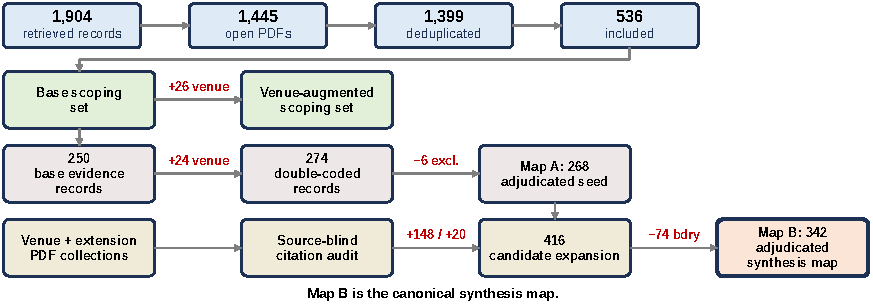
\includegraphics[width=\textwidth]{figures/generated/fig_corpus_lineage.pdf}%
\caption{Corpus lineage. Red deltas on the connectors are, in order, $+26$ and
$+24$ venue-linked additions, $-6$ exclusions, $+148$ new and $+20$ enriched
rows from the citation audit, and $-74$ boundary rows removed at adjudication.
The 416-row venue-expanded candidate map is second-coded and adjudicated into
Map~B (342 rows), the canonical synthesis evidence map. Map~A (268 rows) is the
double-coded adjudicated seed used for IAA and adjudication audit; the base and
venue-augmented scoping sets are used only for boundary checks, while a separate
300-paper source-blind citation audit over the venue and extension PDF
collections decides which papers enter the main text, case studies, or
appendix.}
\label{fig:corpus-flow}
\end{figure*}

\begin{table*}[t]
\centering
\scriptsize
\renewcommand{\arraystretch}{0.88}
\begin{tabularx}{\linewidth}{>{\raggedright\arraybackslash}p{0.15\linewidth}>{\raggedright\arraybackslash}p{0.11\linewidth}>{\raggedright\arraybackslash}p{0.31\linewidth}X}
\toprule
\textbf{Name} & \textbf{Count} & \textbf{Construction rule} & \textbf{Role in this paper} \\
\midrule
Retrieved/open corpus & 1,904 $\rightarrow$ 1,445 $\rightarrow$ 1,399 $\rightarrow$ 536 & Search records, open PDFs, deduplicated candidates, then relevant included papers. & Candidate universe; not a prevalence denominator. \\
Base scoping set & 300 papers & Core reading set plus representative supporting work across failure categories. & Early scoping scaffold; distinct from the source-blind citation audit. \\
Venue-augmented scoping set & 326 papers & Base scoping set plus 26 venue-linked additions from follow-up triage. & Boundary and recall-risk check; not the evidence-map denominator. \\
Map-A candidates & 274 records & 250 base evidence records plus 24 venue-linked evidence additions. & Double-coded by two human sources before adjudication. \\
Map A adjudicated seed & 268 records & Map-A candidates after six final exclusions. & IAA/adjudication basis and provenance snapshot, not the canonical synthesis map. \\
Venue PDF collection (200 papers) & 200 local PDFs & Venue/proceedings-linked open PDFs from ACL-family, ICLR, ICML, NeurIPS, and related sources. & Venue-backed reading/audit collection; future census substrate. \\
Extension PDF collection (100 papers) & 100 local PDFs & Multimodal, graph, table, agentic/tool, code/symbolic, domain, and long-context RAG PDFs. & Extension-layer coverage, used only when tied to evidence-state/action-control claims. \\
Source-blind citation audit & 300 decisions & Source-blind human citation decisions over the venue and extension pools: 115 main, 25 case-study, 110 appendix, 22 background, 28 exclude. & Human audit for which venue/extension papers enter main text, case studies, appendix, or exclusion. \\
\textbf{Map B adjudicated synthesis map} & \textbf{342 records} & Map A (268) plus 74 retained venue/extension additions after second coding and final adjudication; 74 candidate additions were excluded. & \textbf{Primary evidence map for the current synthesis, source-strata analysis, and venue sensitivity.} \\
\bottomrule
\end{tabularx}
\caption{Canonical corpus story. All synthesis counts in the main text refer to the 342-row adjudicated Map B unless a table explicitly says it reports Map A IAA/adjudication evidence or the 416-row pre-adjudication candidate map.}
\label{tab:canonical-corpus-story}
\end{table*}

\begin{table*}[t]
\centering
\scriptsize
\renewcommand{\arraystretch}{0.88}
\begin{tabularx}{\linewidth}{>{\raggedright\arraybackslash}p{0.18\linewidth}>{\raggedright\arraybackslash}p{0.18\linewidth}>{\raggedright\arraybackslash}p{0.29\linewidth}X}
\toprule
\textbf{Audit item} & \textbf{Observed count} & \textbf{Rule / source} & \textbf{Use in main claims} \\
\midrule
Screening flow & 1,904 records $\rightarrow$ 1,445 open PDFs $\rightarrow$ 1,399 deduplicated candidates $\rightarrow$ 536 included & Keyword and curated-list retrieval over arXiv, ACL Anthology, OpenReview, USENIX, AAAI/ACM pages with open versions; deduplicated by normalized title and identifiers. & Defines the initial corpus snapshot; not used as field-wide prevalence. \\
Map A adjudicated seed & 268 records & Human-coded candidate set after round-2 adjudication. Source strata: 42 venue/proceedings-linked, 222 arXiv-only/emerging preprints, and 4 other records. & Preserved as the original adjudicated snapshot and IAA basis; not the canonical synthesis denominator. \\
Map B adjudicated synthesis map & 342 records & Map A plus 74 adjudicated venue/extension additions retained from the 148 candidate additions; 74 candidate additions were excluded after second coding and final adjudication. Source strata: 126 venue/proceedings-linked, 207 arXiv/preprint, 5 workshop/challenge, 4 other/unclear. & Current survey evidence map for source-stratified synthesis; venue-linked papers form a substantial backbone but not a venue-complete census. \\
Venue recall audit & 51 venue-linked candidates surfaced; 26 added to scoping set; 24 added to evidence extension; 9 excluded; 2 duplicates & ACL Anthology scan plus DBLP/OpenAlex/OpenReview/PMLR-style metadata passes and manual triage. & Quantifies recall risk rather than claiming venue-complete coverage. \\
Venue-linked backbone by primary label & 126 venue/proceedings-linked rows: 28 evaluation, 26 adversarial corruption, 22 noisy retrieval, 20 calibration/control, 16 knowledge conflict, 6 distraction, 6 extension-layer, and 2 OOD/uncertainty rows. & Counted from adjudicated Map B after second coding and final adjudication. & Shows that the text/document perspectives have venue-linked support while extension rows remain typed-evidence stress tests; method rankings remain claim- and assumption-specific. \\
\bottomrule
\end{tabularx}
\caption{Main-text corpus and source-strata audit. Detailed query logs, exclusions, and reconciliation tables remain in the appendix and supplement.}
\label{tab:main-corpus-audit}
\end{table*}

\begin{table*}[t]
\centering
\scriptsize
\renewcommand{\arraystretch}{0.9}
\begin{tabularx}{\linewidth}{>{\raggedright\arraybackslash}p{0.20\linewidth}>{\raggedright\arraybackslash}p{0.18\linewidth}>{\raggedright\arraybackslash}p{0.24\linewidth}X}
\toprule
\textbf{Collection item} & \textbf{Count / location} & \textbf{Construction} & \textbf{Use and limitation} \\
\midrule
Venue-linked PDF collection & 200 local PDFs & Open PDFs copied or downloaded from ACL/TACL, ICLR, ICML, NeurIPS, and related proceedings-linked sources. & Strengthens the venue-backed reading set and feeds the source-blind citation audit; it is a PDF collection, not itself the Map-B denominator. \\
Selection sources & 97 foundations; 103 accepted/proceedings papers & Deduplicated by normalised title and filtered by RAG, retrieval, faithfulness, security, calibration, and evaluation terms. & Reduces dependence on arXiv-only discovery, but still reflects open-PDF and keyword bias. \\
Venue concentration & 49 NeurIPS; 38 ICLR; 16 ICML; plus ACL-family venues & Manifest records venue, year, source URL, local path, bytes, and SHA-256 checksum for each PDF. & Provides an auditable venue-linked supplement; manual proceedings-level inclusion/exclusion coding remains future work. \\
Machine-readable files & Manifest, summary, builder script & Built by the venue-200 collection script. & The PDF directory is local due to size; manifests and script are included in the release package. \\
\bottomrule
\end{tabularx}
\caption{Venue-linked 200-paper PDF collection. This collection addresses venue-backed coverage weakness by creating a local open-PDF corpus for citation audit and future venue-complete follow-up, while preserving the distinction between downloaded PDFs, the 416-row candidate expansion, and the canonical 342-row adjudicated Map B.}
\label{tab:venue-200-collection}
\end{table*}

\begin{table*}[t]
\centering
\scriptsize
\renewcommand{\arraystretch}{0.9}
\begin{tabularx}{\linewidth}{>{\raggedright\arraybackslash}p{0.22\linewidth}>{\raggedright\arraybackslash}p{0.16\linewidth}>{\raggedright\arraybackslash}p{0.25\linewidth}X}
\toprule
\textbf{Map-B field group} & \textbf{Coverage} & \textbf{Coding / audit source} & \textbf{Use and caveat} \\
\midrule
Canonical identifiers and source flags & 342/342 title, year, URL, source stratum, Map-A membership, Map-B version, core-reading flag & Deterministic merge from Map A, the venue/extension pools manifests, source-blind citation-audit decisions, and second-coding adjudication. & Defines the canonical adjudicated row set and source strata. \\
Core taxonomy fields & 342/342 failure type, taxonomy categories, method family, intervention point, contribution note, limitation note & Map-A adjudicated labels for original rows; second coding adjudicated labels for retained additions. & Used for Map-B synthesis and sensitivity counts. \\
Task / metric metadata & High coverage after adjudication & Map-A labels plus human-audit rationales and manifest metadata for retained additions. & Missing rows are not imputed for metric-level claims. \\
Author / venue metadata & Source/venue strata complete; author metadata incomplete for some additions & Proceedings metadata and paper manifests. & Venue/source strata are complete; author normalization remains an artifact-release cleanup item. \\
Human-audited rows retained in Map B & 94 retained rows with human citation-audit metadata & 74 retained additions plus 20 enriched Map-A rows. & Citation-audit metadata supports source-stratified synthesis; 74 excluded candidate additions remain in the release as boundary rows. \\
Second-coding/adjudication boundary & Map A: 274 candidates $\rightarrow$ 268 adjudicated rows; Map-B additions: 148 candidates $\rightarrow$ 74 retained additions & Map A has two-source independent coding and final adjudication; Map-B additions have independent second coding and final adjudication. & Second-coding agreement is strong, and adjudication is now applied to the canonical 342-row Map B. \\
\bottomrule
\end{tabularx}
\caption{Coding protocol and field coverage for the 342-row adjudicated Map B. The table separates Map-A adjudicated IAA, source-blind citation-audit metadata, and the second-coding/adjudication pass over the 148 candidate additions.}
\label{tab:map-b-coding-coverage}
\end{table*}

\begin{table*}[t]
\centering
\scriptsize
\renewcommand{\arraystretch}{0.9}
\begin{tabularx}{\linewidth}{>{\raggedright\arraybackslash}p{0.18\linewidth}>{\raggedright\arraybackslash}p{0.20\linewidth}>{\raggedright\arraybackslash}p{0.22\linewidth}>{\raggedright\arraybackslash}p{0.17\linewidth}X}
\toprule
\textbf{Field / decision} & \textbf{Map-A evidence} & \textbf{Map-B addition evidence} & \textbf{Adjudication effect} & \textbf{Claim use} \\
\midrule
Legacy literature-family tag & 274 candidates double-coded (268 retained as Map~A after adjudication); $\kappa=0.96$. & second-coding $\kappa=0.719$; final-label agreement $\kappa=0.743/0.874$. & Candidate labels changed for many additions; final labels are adjudicated. & Supports broad family grouping, not a normalised failure coordinate or field prevalence. \\
Method family & Map-A $\kappa=0.86$. & second-coding $\kappa=0.762$; final-label agreement $\kappa=0.818/0.915$. & Broad candidate method labels were often corrected. & Used for re-analysis and method-role distinctions. \\
Intervention point & Map-A $\kappa=0.92$. & second-coding $\kappa=0.724$; final-label agreement $\kappa=0.807/0.863$. & Pipeline-location labels required adjudication. & Used to locate audit candidates, not to derive five-coordinate verdicts alone. \\
Inclusion / membership & Map-A include decision $\kappa=0.85$. & second-coding inclusion $\kappa=0.769$; final-label agreement $\kappa=0.905/0.865$. & 148 candidate additions $\rightarrow$ 74 retained, 74 excluded. & Defines canonical 342-row Map B; excluded rows are release-only boundary evidence. \\
Candidate-label instability & -- & 139/148 additions required adjudication; 125/148 changed on at least one field vs. candidate labels. & High override rate is reported rather than hidden. & Prevents treating candidate expansion statistics as final synthesis statistics. \\
\bottomrule
\end{tabularx}
\caption{Reliability summary for Map B. Agreement numbers for the second coding are reported against both each other and the final adjudicated labels; the 416-row candidate expansion is not the canonical map.}
\label{tab:main-map-b-reliability}
\end{table*}

\begin{table*}[t]
\centering
\scriptsize
\renewcommand{\arraystretch}{0.9}
\begin{tabularx}{\linewidth}{>{\raggedright\arraybackslash}p{0.20\linewidth}>{\raggedright\arraybackslash}p{0.17\linewidth}>{\raggedright\arraybackslash}p{0.24\linewidth}X}
\toprule
\textbf{Adjudication category} & \textbf{Count} & \textbf{Typical reason} & \textbf{Consequence} \\
\midrule
Accept coder consensus & 114/139 disagreement rows & the second coders agreed that many candidate additions were general RAG, efficiency, domain adaptation, or application papers rather than robust-RAG evidence. & Candidate expansion statistics are not used directly; boundary rows are released but excluded from canonical Map B. \\
Keep candidate label & 14/139 & Candidate label remained appropriate despite one coder disagreement, usually when the paper clearly addressed a robust-RAG failure or benchmark axis. & Shows adjudication did not mechanically follow coders. \\
Resolve mixed labels & 7/139 & Coders and candidate labels captured different valid aspects, e.g., control plus evaluation or extension plus retrieval. & Final label chooses the primary comparison role; secondary evidence remains in notes. \\
Accept coder~2 & 4/139 & the second coder better matched the paper's primary contribution after full adjudication. & Small number of one-coder overrides are recorded explicitly. \\
\midrule
Retained additions & 74/148 & Robustness, evaluation, control, conflict, or security contribution survives adjudication. & Included in canonical 342-row Map B. \\
Excluded additions & 74/148 & Boundary/application/general-RAG papers, often venue-linked, did not directly study unreliable evidence. & Excluded from synthesis counts but retained as release artifacts. \\
\bottomrule
\end{tabularx}
\caption{Map-B candidate-addition override audit. The high adjudication rate is treated as evidence that the 416-row candidate expansion was too inclusive; the canonical map uses the 342-row adjudicated version.}
\label{tab:map-b-override-audit}
\end{table*}


\clearpage
\begin{table*}[t]
\centering
\small
\begin{tabularx}{\linewidth}{p{0.18\linewidth}p{0.16\linewidth}X}
\toprule
\textbf{Stage} & \textbf{Count} & \textbf{Rule} \\
\midrule
Initial retrieval & 1,904 records & Keyword search over arXiv, ACL Anthology, OpenReview, USENIX, AAAI/ACM landing pages where open versions were available, plus curated robust/trustworthy RAG paper lists; search cutoff 2026-06-03. \\
Open full-text corpus & 1,445 PDFs & Downloaded only open PDFs; removed failed downloads, inaccessible files, and non-PDF artifacts. \\
Deduplicated candidates & 1,399 papers & Deduplicated by normalised title and arXiv/proceedings identifiers; retained the most complete metadata record when preprint and proceedings versions overlapped. \\
Relevance screening & 536 included papers & Included papers that study RAG robustness, reliability, uncertainty, calibration, faithfulness, attack/defense, or evaluation under unreliable evidence; excluded application-only RAG papers. \\
Core pool & 112 papers & Papers directly shaping the taxonomy, threat/failure model, intervention mechanisms, or evaluation framework. \\
Core reading set & 100 papers & Core papers used as main narrative anchors; the remaining 12 core-pool papers stay in the broader scoping set. \\
Base scoping set & 300 papers & Core papers plus representative supporting work across all taxonomy branches before venue follow-up triage. \\
Venue-augmented scoping set & 326 papers & Base scoping set plus 26 venue-linked additions after follow-up triage. \\
Candidate evidence records & 274 papers & Base evidence map of 250 papers plus 24 venue-linked additions, double-coded and adjudicated. \\
Map A adjudicated seed & 268 papers & Candidate evidence records retained after final adjudication; used for IAA/adjudication provenance. \\
Map-B candidate expansion & 416 papers & Map A plus 148 source-blind human-citation-audit additions and 20 enriched original rows; used for second-coding review. \\
Map B adjudicated synthesis map & 342 papers & Map A plus 74 retained additions after second coding and final adjudication; frozen for current descriptive statistics. Post-freeze discoveries enter a recall log until a new version is coded. \\
\bottomrule
\end{tabularx}
\caption{Screening-flow summary. Search ends on 2026-06-03; coding and adjudication artifacts freeze on 2026-06-15. The supplement provides query strings, source counts, rules, exclusions, hashes, and a post-freeze recall log.}
\label{tab:review-protocol}
\end{table*}

\begin{table*}[t]
\centering
\scriptsize
\renewcommand{\arraystretch}{0.92}
\begin{tabularx}{\linewidth}{>{\raggedright\arraybackslash}p{0.17\linewidth}>{\raggedleft\arraybackslash}p{0.07\linewidth}>{\raggedright\arraybackslash}p{0.24\linewidth}X}
\toprule
\textbf{Set} & \textbf{N} & \textbf{Audit artifact} & \textbf{Selection rule and role} \\
\midrule
Retrieved records & 1,904 & \texttt{search\_protocol.json} & Initial keyword and curated-list retrieval before PDF availability, deduplication, or relevance screening. \\
Open full-text PDFs & 1,445 & \texttt{pdfs/} & Records with open PDFs available for full-text inspection; inaccessible or non-PDF artifacts removed. \\
Deduplicated candidates & 1,399 & \texttt{all\_reviewed\_deduped.csv} & Normalized-title and identifier deduplication; one record retained for preprint/proceedings overlaps. \\
Relevant included papers & 536 & \texttt{all\_reviewed\_deduped.csv} & Papers with decision \texttt{core} (112) or \texttt{include} (424); background-adjacent papers (289) and excluded papers (574) are tracked separately. \\
Core pool & 112 & \texttt{decision=core} in \texttt{all\_reviewed\_deduped.csv} & Papers judged central to taxonomy, threat/failure models, intervention mechanisms, or evaluation design. \\
Core reading set & 100 & \texttt{core100\_full.csv} & Main narrative anchors. The 12 core-pool papers not in this set remain in the base scoping set rather than being discarded. \\
Base scoping set & 300 & \texttt{survey300\_full.csv} & Core pool plus representative supporting work across failure categories, method families, and evaluation settings before venue follow-up triage. \\
Venue-augmented scoping set & 326 & \texttt{survey\_set\_venue\_audited.csv} & Base scoping set plus 26 venue-linked papers added after follow-up triage. \\
Base evidence map & 250 & \texttt{evidence\_map.csv} & Original structured map used before venue follow-up triage. \\
Candidate evidence records & 274 & round2 full adjudication CSV & Base map plus venue-linked additions, double-coded by humans and adjudicated. \\
Map A adjudicated seed & 268 & \texttt{evidence\_map\_adjudicated.csv} & Candidate evidence records with final \texttt{include\_in\_evidence\_map=1}; used for IAA/adjudication provenance. \\
Source-blind citation audit & 300 & \texttt{citation\_annotations.csv} & Source-blind human citation decisions over the venue and extension pools; distinct from the base scoping set. \\
Map-B candidate expansion & 416 & candidate expansion CSV & Map A plus 148 candidate additions supported by the source-blind citation audit and 20 enriched original rows; used for second coding. \\
Map B adjudicated synthesis map & 342 & adjudicated Map-B CSV & Map A plus 74 retained additions after second-coding adjudication; used for current synthesis statistics. \\
\bottomrule
\end{tabularx}
\caption{Corpus-set ledger. Exact memberships are released as CSV files for Map A, the 416-row candidate expansion, and the 342-row adjudicated Map B.}
\label{tab:set-selection-ledger}
\end{table*}

\begin{table*}[t]
\centering
\scriptsize
\renewcommand{\arraystretch}{0.94}
\begin{tabularx}{\linewidth}{>{\raggedright\arraybackslash}p{0.18\linewidth}>{\raggedright\arraybackslash}p{0.23\linewidth}>{\raggedright\arraybackslash}p{0.24\linewidth}X}
\toprule
\textbf{Artifact / claim source} & \textbf{Verification performed} & \textbf{What is coding- or metadata-assisted} & \textbf{How it is used in the paper} \\
\midrule
Main narrative claims and central citations & Author inspection of full paper text for papers used to support central claims, tables, and figures. & Initial prioritization and category suggestions were LLM-assisted. & Used for qualitative synthesis and case-study comparisons. \\
Core reading set & 100 papers curated from the 112-paper core pool after full-text relevance checks for narrative fit. & Core-pool creation used relevance scores and pre-labels as triage signals. & Used as the main reading backbone; not claimed to be a reproducible top-100 ranking without author judgment. \\
Map A, 268-paper adjudicated seed & Metadata and structured fields manually cleaned; venue-candidate triage completed; 274 candidate records independently double-coded and adjudicated into 268 included evidence-map papers. & Initial candidate discovery and pre-labeling were LLM-assisted, but final Map-A labels use human adjudication for coder disagreements. & Used for IAA/adjudication provenance, with the caveat that it is not the current synthesis denominator. \\
Map-B candidate expansion, 416 rows & Map A merged with source-blind human citation audit over the venue/extension pools; 148 new candidate rows added and 20 original rows enriched. & Candidate additions use human citation-audit decisions and deterministic field completion before second coding. & Used as the candidate pool for second coding, not as the final synthesis denominator. \\
Map B, 342-paper adjudicated synthesis map & Two coders independently second-coded all 148 additions; final adjudication retained 74 and excluded 74. & The retained additions use adjudicated labels; excluded boundary rows remain available in the release package. & Used for current source-stratified synthesis and venue sensitivity; still not a field census. \\
Human double-coding package & Two anonymized human sources independently coded all 274 candidate evidence records before discussion; round-2 agreement is strong across taxonomy, intervention, evidence-strength, relevance, core, and inclusion fields. & Disagreements were resolved in the final adjudication file. & Used to report pre-adjudication IAA and produce final adjudicated evidence-map labels. \\
Venue metadata pass and triage & ACL Anthology title/abstract scan plus DBLP/OpenAlex query logs, title matching, and follow-up triage decisions. & Discovery is metadata-based; inclusion/exclusion decisions are author triage rather than independent double coding. & Used to update venue-linked coverage and quantify remaining systematic-review limits. \\
\bottomrule
\end{tabularx}
\caption{Verification and annotation provenance. The table separates full-text author inspection, coding-assisted labels, metadata-derived venue candidates, and non-adjudicated consistency diagnostics.}
\label{tab:verification-provenance}
\end{table*}

\begin{table*}[t]
\centering
\scriptsize
\renewcommand{\arraystretch}{0.9}
\begin{tabularx}{\linewidth}{>{\raggedright\arraybackslash}p{0.19\linewidth}>{\raggedright\arraybackslash}p{0.25\linewidth}>{\raggedright\arraybackslash}p{0.24\linewidth}X}
\toprule
\textbf{Item} & \textbf{What was done} & \textbf{What was hidden from annotators} & \textbf{What we do not claim} \\
\midrule
Round-2 coders & Two anonymized coding-source records cover the same 274 candidate evidence records. & Machine pre-labels, prior evidence-map labels, previous adjudication logs, and the other source's labels. & The public package does not establish qualifications or personnel overlap; we claim file-level provenance, not independently verified expertise. \\
Training / codebook & Coders used the double-coding protocol and codebook defining scope, legacy literature-family tag, method family, intervention point, evidence strength, and inclusion fields. & Prior LLM rationales and model confidence scores. & We do not claim the codebook is final for all RAG subareas; adjudication notes can still motivate revisions. \\
Pre-adjudication separation & IAA was computed from separately completed CSV files before adjudication. & Post-discussion labels were not used for IAA. & This establishes workflow separation in the files, not personnel independence beyond the anonymized records. \\
Adjudication & A final adjudication file resolved 469 field-level disagreements and produced the 268-paper Map-A seed. & Source labels were preserved and not overwritten. & We do not apply Map-A IAA to the 148 later Map-B additions. \\
Source-blind citation audit & One source-blind citation-audit record set coded 300 papers from the venue/extension pools; 168 audited rows entered or enriched Map B after de-duplication and relevance checks. & Paper IDs were source-normalised and the audit did not use Map-A disagreement labels. & We do not claim 416-row double-coding, inter-annotator agreement, or independently verified annotator provenance for this batch. \\
\bottomrule
\end{tabularx}
\caption{Annotation transparency for the coding round. The table distinguishes file-auditable workflow separation from qualifications and personnel independence that the blind package does not establish.}
\label{tab:annotation-transparency}
\end{table*}

\begin{table*}[t]
\centering
\scriptsize
\renewcommand{\arraystretch}{0.94}
\begin{tabularx}{\linewidth}{>{\raggedright\arraybackslash}p{0.22\linewidth}>{\raggedright\arraybackslash}p{0.24\linewidth}>{\raggedright\arraybackslash}p{0.20\linewidth}X}
\toprule
\textbf{Claim} & \textbf{Status under venue-linked / peer-reviewed evidence} & \textbf{What changes without preprints} & \textbf{Interpretation} \\
\midrule
Retrieved evidence can harm generation even when relevant evidence exists. & Holds: supported by venue-linked work on irrelevant/noisy context, noise-robust training, counterfactual noise, and imperfect retrieval. & The range of stress-test variants shrinks. & This is a stable mechanism-level claim. \\
RAG security results require attacker-capability normalisation. & Holds partially: venue-linked security work covers poisoning, traceback, membership inference, and backdoor-style corpus attacks. & Many fine-grained attack variants and defenses remain preprint-heavy. & The capability matrix is stable; detailed landscape counts are emerging trends. \\
Calibration, abstention, and retrieval control are distinct decisions. & Holds conceptually with venue-linked answerability, relevance-assessment, and calibration/control papers. & Specific method rankings and benchmark prevalence become sparse. & The conceptual separation remains; empirical prevalence is not settled. \\
The evidence map is attack- and benchmark-heavy. & Does not become a field-wide claim. & Under peer-reviewed-only evidence, the sample is much smaller and more evaluation-heavy. & Treat distributional cross-tabs as corpus diagnostics, not prevalence estimates. \\
Action-trace benchmark blueprint should score answer, evidence state, action, and cost. & Supported as a design synthesis, not validated as a benchmark standard. & The proposal becomes less empirical and more normative. & Keep as a research agenda unless a full benchmark is built and evaluated. \\
\bottomrule
\end{tabularx}
\caption{Peer-reviewed / venue-linked sensitivity analysis. The table states which conclusions survive when preprint-only evidence is downweighted and which remain hypothesis-generating.}
\label{tab:peer-reviewed-sensitivity}
\end{table*}


\begin{table*}[t]
\centering
\scriptsize
\renewcommand{\arraystretch}{0.88}
\begin{tabularx}{\linewidth}{>{\raggedright\arraybackslash}p{0.24\linewidth}>{\raggedright\arraybackslash}p{0.18\linewidth}>{\raggedright\arraybackslash}p{0.26\linewidth}X}
\toprule
\textbf{Conclusion tested after downweighting preprints} & \textbf{Venue-linked support in map} & \textbf{What remains supported} & \textbf{What remains trend evidence} \\
\midrule
Noise/distraction are not reducible to retriever recall. & 22 primary noisy-retrieval and 6 distraction venue-linked rows, plus context-compression/reranking benchmarks. & Context construction, ranking, compression, and generator selectivity all affect robustness. & Exact method rankings across retrievers, generators, and context budgets. \\
Natural conflict and poisoning are different comparison games. & 16 primary knowledge-conflict and 26 adversarial-corruption venue-linked rows. & Source reconciliation and attacker-created integrity failures require different assumptions and metrics. & Transfer from conflict-resolution methods to adaptive poisoning defenses. \\
RAG security results require capability normalisation. & 26 primary adversarial-corruption venue-linked rows, including poisoning, privacy/extraction, and defenses. & Attack success is uninterpretable without corpus access, query control, retriever visibility, insertion budget, objective, and defense action. & Detailed cross-threat leaderboards across heterogeneous attacker capabilities. \\
Calibration, abstention, and retrieval control are separable. & 20 primary calibration/control venue-linked rows plus answerability and adaptive retrieval work. & Confidence target, evidence sufficiency, coverage, retrieval cost, and action utility should be reported separately. & Frontier-model control policies and multi-action cost tradeoffs across domains. \\
Answer accuracy alone is insufficient for robust-RAG evaluation. & 28 primary evaluation/benchmark venue-linked rows. & Evidence state, support, threat model, action policy, and cost are needed to interpret results. & A full action-trace benchmark remains future work. \\
Extension-layer RAG requires typed evidence states. & 6 primary extension-layer venue-linked rows. & Visual, graph, table, memory, tool, code, and domain evidence require modality-specific grounding and action labels. & Unified evaluation across text, multimodal, graph, table, and agentic RAG remains immature and is not treated as co-equal coverage. \\
\bottomrule
\end{tabularx}
\caption{Venue-restricted descriptive analysis. Counts refer to primary Map-B labels; they show represented comparison families, not weighted effects, field prevalence, or confirmation of a mechanism.}
\label{tab:main-peer-sensitivity}
\end{table*}

\begin{table*}[t]
\centering
\scriptsize
\renewcommand{\arraystretch}{0.9}
\begin{tabularx}{\linewidth}{>{\raggedright\arraybackslash}p{0.19\linewidth}>{\raggedright\arraybackslash}p{0.19\linewidth}>{\raggedright\arraybackslash}p{0.20\linewidth}>{\raggedright\arraybackslash}p{0.18\linewidth}X}
\toprule
\textbf{Robust-RAG setting} & \textbf{Venue-backed basis} & \textbf{Recommended comparison target} & \textbf{Action policy to report} & \textbf{Boundary condition} \\
\midrule
Benign noisy retrieval / distraction & 22 noisy-retrieval and 6 distraction venue-linked rows; IrrelCtx, RAAT, RECOMP, RankRAG, RGB. & Compare filters, rerankers, compressors, training methods, and readers only under matched negative type, rank, gold evidence, and generator. & answer, filter, rerank/compress, abstain/retrieve-more. & More context can help when gold evidence is missing; ranking claims require a shared harness. \\
Faithfulness / attribution / conflict & 16 knowledge-conflict venue-linked rows plus RAGTruth, FaithEval, Trust-Align, reconciliation work. & Compare span support, claim support, source conflict, and final answer correctness as different targets. & answer, verify, expose conflict, refuse/defer. & Citation support is not sufficient evidence of conflict robustness. \\
Adversarial RAG security & 26 adversarial-corruption venue-linked rows including poisoning, privacy/extraction, and defenses. & Compare attacks/defenses inside one capability envelope: corpus access, query control, budget, retriever visibility, objective. & prevent, demote, detect, quarantine, trace, recover, or limit leakage. & Cross-threat leaderboards are invalid unless threat model and clean utility align. \\
Calibration / retrieval control / abstention & 20 calibration/control venue-linked rows plus answerability and adaptive retrieval work. & Compare confidence targets, sufficiency labels, retrieval triggers, and action utility separately. & answer, retrieve again, clarify, abstain, verify, escalate. & Calibration error alone does not define a policy. \\
Evaluation resources & 28 evaluation/benchmark venue-linked rows including RGB, RAGTruth, RAGAS, ARES, BEIR, BERGEN, RAGLAB. & Use diagnostic scorecards rather than one robust-RAG score. & required action label and cost/coverage reporting. & Toolkits, annotated corpora, retriever benchmarks, and system harnesses play different roles. \\
\bottomrule
\end{tabularx}
\caption{Comparison-design prompts grounded in the venue/proceedings-linked Map-B subset. Counts are descriptive and do not by themselves establish the listed mechanism claims.}
\label{tab:venue-backed-recommendations}
\end{table*}

\begin{table*}[t]
\centering
\scriptsize
\renewcommand{\arraystretch}{0.94}
\begin{tabularx}{\linewidth}{>{\raggedright\arraybackslash}p{0.20\linewidth}>{\raggedright\arraybackslash}p{0.25\linewidth}>{\raggedright\arraybackslash}p{0.18\linewidth}X}
\toprule
\textbf{Pass} & \textbf{Scope} & \textbf{Observed yield} & \textbf{Interpretation} \\
\midrule
ACL Anthology metadata scan & ACL, EMNLP, NAACL, COLING; 2020--2026; full anthology BibTeX with abstracts & 12,924 entries scanned; 181 RAG candidates; 30 robust-RAG candidates & A reproducible proceedings-level metadata scan for core NLP venues, not just backfilled metadata. \\
DBLP/OpenAlex metadata queries & 15 robust-RAG query strings over venue-linked metadata for SIGIR, WWW, WSDM, KDD, USENIX Security, CCS, NDSS, ICLR, NeurIPS and overlaps & 31 query rows; 51 unique venue-linked candidate titles after deduplication & Surfaced missing venue-linked candidates; all 51 were subsequently triaged. \\
Follow-up venue triage & 51 venue-linked candidates & 23 new evidence-map additions; 3 background additions; 9 exclusions; 2 duplicates; 13 already represented & Closes the unprocessed venue-candidate gap, while still not claiming complete manual proceedings coverage. \\
Map A adjudicated seed & 268 evidence-map papers & 42 venue/proceedings-linked; 222 arXiv-only or emerging preprints; 4 other strata & IAA/adjudication basis before venue expansion. \\
Map-B candidate expansion & 416 evidence-map candidates & 194 venue/proceedings-linked; 207 arXiv/preprint; 11 workshop/challenge; 4 other/unclear & Pre-adjudication candidate map after source-blind citation audit. \\
Map B adjudicated synthesis map & 342 evidence-map papers & 126 venue/proceedings-linked; 207 arXiv/preprint; 5 workshop/challenge; 4 other/unclear & Current source-stratified synthesis map after second coding and final adjudication. \\
\bottomrule
\end{tabularx}
\caption{Venue-oriented search, coverage audit, and follow-up triage summary. Full query logs, candidate titles, decisions, and limitations are in \texttt{venue\_systematic\_queries.csv}, \texttt{venue\_systematic\_candidates.csv}, \texttt{venue\_coverage\_audit.csv}, and \texttt{venue\_triage\_decisions.csv}.}
\label{tab:venue-pass-summary}
\end{table*}

\begin{table*}[t]
\centering
\scriptsize
\renewcommand{\arraystretch}{0.94}
\begin{tabularx}{\linewidth}{>{\raggedright\arraybackslash}p{0.20\linewidth}>{\raggedright\arraybackslash}p{0.18\linewidth}>{\raggedright\arraybackslash}p{0.18\linewidth}X}
\toprule
\textbf{Coverage check} & \textbf{Count} & \textbf{Artifact} & \textbf{Interpretation} \\
\midrule
Venue-linked robust-RAG candidates found by metadata pass & 51 unique titles & candidate CSV & Candidate pool from ACL Anthology, DBLP, and OpenAlex metadata queries. \\
Already in core100 & 6 / 51 & coverage audit CSV & Core narrative captures only a small subset of venue-linked candidates. \\
Already in base scoping set & 14 / 51 & coverage audit CSV & The current scoping set misses or intentionally excludes many venue-linked candidates. \\
Already in evidence map & 13 / 51 & coverage audit CSV & Cross-tabs should be interpreted as map statistics, not field statistics. \\
Not in original base scoping set & 37 / 51 & coverage audit CSV & These papers were subsequently triaged; see Table~\ref{tab:venue-triage-summary}. \\
\bottomrule
\end{tabularx}
\caption{Venue-coverage audit after the metadata pass. The audit quantifies residual coverage risk by matching venue-linked candidates against the original core, survey, and evidence-map sets. Files: \texttt{venue\_systematic\_candidates.csv} and \texttt{venue\_coverage\_audit.csv}.}
\label{tab:venue-coverage-audit}
\end{table*}

\begin{table*}[t]
\centering
\scriptsize
\renewcommand{\arraystretch}{0.9}
\begin{tabularx}{\linewidth}{>{\raggedright\arraybackslash}p{0.20\linewidth}>{\raggedright\arraybackslash}p{0.24\linewidth}>{\raggedright\arraybackslash}p{0.20\linewidth}X}
\toprule
\textbf{Recall check} & \textbf{Observed result} & \textbf{What it controls} & \textbf{Residual risk} \\
\midrule
ACL Anthology metadata scan & 12,924 entries scanned for ACL/EMNLP/NAACL/COLING; 181 RAG candidates; 30 robust-RAG candidates & Reduces reliance on arXiv-only discovery for core NLP venues. & Title/abstract terms can miss papers using older QA/IR terminology. \\
Cross-venue metadata pass & DBLP/OpenAlex queries yielded 51 venue-linked robust-RAG candidates & Adds IR, web, security, and ML venue-linked records. & API ranking, metadata naming, and transient query errors limit recall. \\
Follow-up triage & 51 candidates triaged; 26 added to scoping set; 24 added to evidence map; 9 excluded; 2 duplicates & Closes the known unprocessed venue-candidate gap. & Does not prove complete coverage of every proceedings volume. \\
Evidence-strength sensitivity & Main conclusions separated into venue-linked backbone vs preprint trend evidence & Prevents preprint-heavy map statistics from becoming field-level claims. & Some emerging security/control subtopics remain too new for strong consensus. \\
\bottomrule
\end{tabularx}
\caption{Venue-recall risk analysis. The venue pass improves auditability and adds missed venue-linked papers, but it is still not a manual venue-complete proceedings review.}
\label{tab:venue-recall-risk}
\end{table*}


\begin{table*}[t]
\centering
\scriptsize
\renewcommand{\arraystretch}{0.94}
\begin{tabularx}{\linewidth}{>{\raggedright\arraybackslash}p{0.22\linewidth}>{\raggedright\arraybackslash}p{0.15\linewidth}>{\raggedright\arraybackslash}p{0.20\linewidth}X}
\toprule
\textbf{Triage outcome} & \textbf{Count} & \textbf{Action} & \textbf{Reasoning} \\
\midrule
Already represented in base evidence map & 13 & retain & Candidate was already included; metadata pass only improved venue visibility. \\
New evidence-map additions & 23 & add to evidence extension & Directly studies robust RAG, RAG evaluation, evidence reliability, security, calibration, or robust generation. \\
Scoping-set paper promoted to evidence extension & 1 & add to evidence extension & Already in the scoping set but not the base map; venue audit identified it as relevant to trust/calibration. \\
Background additions & 3 & add to venue-augmented scoping set only & Relevant boundary papers on domain, multilingual, or multimodal RAG, but not central text evidence-reliability evidence. \\
Excluded false positives / applications & 9 & exclude with reason & Application or adjacent RAG papers without robustness/evidence-reliability analysis. \\
Duplicate venue records & 2 & deduplicate & Same work already represented through another metadata record. \\
\midrule
\textbf{Venue-augmented scoping set} & \textbf{326} & base 300 + 26 additions & Updated scoping set after follow-up triage. \\
\textbf{Map A adjudicated seed} & \textbf{268} & 274 candidates - 6 exclusions & IAA/adjudication snapshot after human adjudication of double-coded candidate evidence records. \\
\textbf{Map-B candidate expansion} & \textbf{416} & Map A + 148 citation-audit-supported additions & Pre-adjudication candidate map after source-blind citation audit. \\
\textbf{Map B adjudicated synthesis map} & \textbf{342} & Map A + 74 retained additions & Current evidence map for synthesis after second coding and adjudication. \\
\bottomrule
\end{tabularx}
\caption{Follow-up triage of all 51 venue-linked candidates from the metadata pass. The 37 candidates outside the original scoping set are no longer unprocessed; decisions and reasons are in \texttt{venue\_triage\_decisions.csv}.}
\label{tab:venue-triage-summary}
\end{table*}

\begin{table*}[t]
\centering
\scriptsize
\renewcommand{\arraystretch}{0.92}
\begin{tabularx}{\linewidth}{>{\raggedright\arraybackslash}p{0.20\linewidth}>{\raggedright\arraybackslash}p{0.15\linewidth}>{\raggedright\arraybackslash}p{0.30\linewidth}X}
\toprule
\textbf{Artifact / set} & \textbf{Count} & \textbf{Count definition} & \textbf{Use in this paper} \\
\midrule
Map-A double-coded candidates & 274 & Candidate records coded by two human sources before final inclusion adjudication. & Used for human-human agreement and adjudication; six records were excluded from Map A. \\
Map A adjudicated seed & 268 & Included records after adjudication: 42 venue/proceedings-linked, 222 arXiv-only or emerging preprints, 2 preprints with year tags, 1 review-platform record, and 1 other/uncategorized record. & Used as the IAA/adjudication provenance snapshot, not the current synthesis denominator. \\
Venue-augmented scoping set & 326 & Original base scoping set plus 26 triaged venue-linked additions. & Used for broader scoping and boundary checks; not all rows are evidence-map records. \\
Source-blind citation audit & 300 & Human citation decisions over venue PDFs and extension PDFs. & Determines which audited papers enter the main text, case studies, appendix, background, or exclusion set; distinct from the base scoping set. \\
Map-B candidate expansion & 416 & Map A plus 148 candidate additions supported by the source-blind citation audit; 20 original rows enriched with citation-audit metadata. & Pre-adjudication expansion candidate map used for second-coding review. \\
Map B adjudicated synthesis map & 342 & Map A plus 74 retained additions after second coding and final adjudication. & Current evidence map for source-stratified synthesis and Map-B cross-tabs. \\
\bottomrule
\end{tabularx}
\caption{Reconciliation of reported corpus counts. The 342-row adjudicated Map B is the canonical synthesis map; Map A and the 274-candidate set are retained to report double-coding and adjudication provenance.}
\label{tab:source-strata-reconciliation}
\end{table*}

\clearpage
\begin{table*}[t]
\centering
\scriptsize
\begin{tabularx}{\linewidth}{p{0.24\linewidth}p{0.14\linewidth}p{0.14\linewidth}X}
\toprule
\textbf{Field} & \textbf{Agreement} & \textbf{$\kappa$ / score} & \textbf{Interpretation} \\
\midrule
Full-text checked & 100.0\% & 1.00 & Both sources marked every evidence-map paper as full-text checked. \\
In-scope screening & 99.6\% & 0.92 & Near-complete agreement; only one screening disagreement remains for adjudication. \\
Relevance level & -- & 0.80 & Linear-weighted agreement is strong for exclude/background/support/core priority. \\
Primary failure type & 97.1\% & 0.96 & Very strong human agreement on the main taxonomy category. \\
Method family & 89.4\% & 0.86 & Strong agreement on attack, benchmark, control, method, and analysis families. \\
Intervention point & 93.4\% & 0.92 & Very strong agreement on pipeline placement. \\
Evaluation type & 94.9\% & 0.93 & Very strong agreement on metric/evaluation family. \\
Evidence strength & 97.8\% & 0.95 & Very strong agreement on proceedings/preprint/review-platform strata. \\
Core-candidate decision & 91.6\% & 0.80 & Strong agreement on whether papers should shape the core narrative. \\
Include in evidence map & 99.3\% & 0.85 & Strong agreement on evidence-map inclusion. \\
Secondary labels & 79.2\% exact & 0.83 Jaccard & Multilabel agreement is strong enough to support overlap analysis after adjudication. \\
Reproducibility evidence & 10.6\% exact & 0.20 Jaccard & Weak free-text agreement; retained as adjudicated audit metadata, not used for primary comparison or trend claims. \\
\bottomrule
\end{tabularx}
\caption{Round-2 human-human agreement on 274 candidate evidence records before adjudication. Structured labels show strong agreement, while the free-text reproducibility field is weak and is treated only as adjudicated audit metadata. Two anonymized human annotation sources independently coded the same records; remaining disagreements were resolved to produce the 268-row Map-A adjudicated seed. These IAA values do not apply to the 148 later Map-B additions.}
\label{tab:iaa}
\end{table*}

\begin{table*}[t]
\centering
\scriptsize
\renewcommand{\arraystretch}{0.9}
\begin{tabularx}{\linewidth}{>{\raggedright\arraybackslash}p{0.19\linewidth}>{\raggedright\arraybackslash}p{0.18\linewidth}>{\raggedright\arraybackslash}p{0.18\linewidth}>{\raggedright\arraybackslash}p{0.20\linewidth}X}
\toprule
\textbf{Field} & \textbf{coder~1 vs.\ final} & \textbf{coder~2 vs.\ final} & \textbf{coder~1 vs.\ coder~2} & \textbf{Final adjudication effect} \\
\midrule
Primary failure type & 0.784 / 0.743 & 0.899 / 0.874 & 0.764 / 0.719 & Final labels resolve 125 rows that changed from the candidate expansion on at least one field. \\
Method family & 0.878 / 0.818 & 0.946 / 0.915 & 0.838 / 0.762 & Broad candidate method labels were corrected toward coder-supported labels. \\
Intervention point & 0.838 / 0.807 & 0.885 / 0.863 & 0.770 / 0.724 & Pipeline-location disagreements are resolved before final Map-B synthesis. \\
Scope / inclusion & 0.953 / 0.905 & 0.932 / 0.865 & 0.885 / 0.769 & Final Map B retains 74 additions and excludes 74 boundary candidates. \\
\bottomrule
\end{tabularx}
\caption{Final-label agreement for the 148 Map-B candidate additions. Cells report agreement / Cohen's $\kappa$ against the final adjudicated label, not the pre-adjudication candidate label. This resolves the apparent instability of the candidate map: coder~1 and coder~2 agree strongly with the final labels, and excluded boundary rows are kept in the release but not in canonical Map B.}
\label{tab:map-b-second-coding-c02-c03}
\end{table*}


\begin{table}[t]
\centering
\scriptsize
\setlength{\tabcolsep}{3pt}
\begin{tabularx}{\linewidth}{lrr>{\raggedright\arraybackslash}X}
\toprule
\textbf{Metric} & \textbf{Control} & \textbf{Protocol} & \textbf{$\Delta$ (95\% CI)} \\
\midrule
Experts & 15 & 15 & -- \\
Pair judgments & 180 & 180 & -- \\
Panel-label agreement & 0.800 & 0.978 & +0.178 [+0.128, +0.228] \\
Fleiss $\kappa$ & 0.589 & 0.846 & -- \\
Decision time (s) & 126.1 & 121.8 & -4.3 [-13.9, +5.8] \\
Confidence (1--5) & 3.69 & 3.92 & +0.23 [+0.13, +0.32] \\
Usefulness (1--5) & 3.51 & 4.06 & +0.55 [+0.41, +0.70] \\
\bottomrule
\end{tabularx}
\caption{Twelve-pair protocol-usability pilot. Thirty annotators judged the same deliberately difficult pairs, with 15 per condition. Agreement with panel labels is descriptive for this non-representative set; public metadata do not establish panel qualifications or personnel independence. Intervals are participant-level bootstrap intervals, not population paper-pair inference.}
\label{tab:expert-validation-pilot}
\end{table}

\begin{table*}[t]
\centering
\scriptsize
\renewcommand{\arraystretch}{0.88}
\begin{tabularx}{\linewidth}{>{\raggedright\arraybackslash}p{0.12\linewidth}>{\raggedright\arraybackslash}p{0.18\linewidth}>{\raggedright\arraybackslash}p{0.16\linewidth}>{\raggedright\arraybackslash}p{0.20\linewidth}X}
\toprule
\textbf{Pair} & \textbf{Control pattern} & \textbf{Protocol pattern} & \textbf{Tuple explanation} & \textbf{Disagreement lesson} \\
\midrule
P08 & 1/15 matched gold; 14/15 chose partial instead of invalid. & 13/15 matched invalid. & AstuteRAG-style benign conflict reasoning and PoisonedRAG-style attacker-created evidence differ in threat model, intervention point, metric polarity, and action. & Without the tuple, experts tended to over-group conflict and poisoning as related robustness papers. \\
P04 & 3/15 matched partial; 12/15 over-called valid. & 15/15 matched partial. & Chain-of-Note and irrelevant-context filtering share a noise family but differ in generator reasoning vs. context filtering and answer+abstain vs. filter+answer actions. & The tuple turns a tempting leaderboard comparison into a pipeline-composition claim. \\
P01 & 11/15 matched partial; 4/15 over-called valid. & 15/15 matched partial. & IrrelCtx and RAAT share answer metrics but differ in natural retrieval noise vs. constructed counterfactual noise and filter/back-off vs. answer-only actions. & The tuple exposes action-policy mismatch even when datasets and metrics overlap. \\
P09 & 13/15 matched partial; 2/15 over-called valid. & 15/15 matched partial. & PoisonedRAG and certified/robust defenses share bounded corruption but differ in attacker vs. defender role, attack success vs. certified robust accuracy, and answer/abstain/filter actions. & Even same-threat-space papers need role and action normalization before ranking. \\
P02 & 14/15 matched partial; 1/15 over-called invalid. & 15/15 matched partial. & IrrelCtx is a method paper; RGB is a benchmark artifact with negative rejection and counterfactual testbeds. & Method-vs-benchmark comparisons should ask what evaluation would make them comparable. \\
\bottomrule
\end{tabularx}
\caption{Disagreement analysis for the external expert-use stress test. The table reports illustrative real paper-pair comparisons where ordinary expert judgment and tuple-guided judgment diverged. It is usability evidence for the protocol on 12 hard pairs, not population-level validation.}
\label{tab:expert-disagreement-analysis}
\end{table*}


\begin{table*}[t]
\centering
\scriptsize
\renewcommand{\arraystretch}{0.9}
\begin{tabularx}{\linewidth}{>{\raggedright\arraybackslash}p{0.20\linewidth}>{\raggedright\arraybackslash}p{0.15\linewidth}>{\raggedright\arraybackslash}p{0.16\linewidth}>{\raggedright\arraybackslash}p{0.19\linewidth}X}
\toprule
\textbf{Quantity} & \textbf{Control} & \textbf{Protocol} & \textbf{Gold / model} & \textbf{Interpretation} \\
\midrule
Annotators / judgments & 3 / 180 & 3 / 180 & 3 gold adjudicators / 180 gold votes & Expanded validation uses unseen pairs and multiple gold adjudicators. \\
Agreement with panel gold & 0.567 & 0.883 & Panel consensus over 60 pairs & The tuple protocol improves verdict agreement on the blinded re-annotation. \\
Mean confidence & 4.07 & 3.83 & -- & Protocol users are slightly less confident but substantially more aligned with panel gold. \\
Protocol minus control & \multicolumn{2}{c}{+0.317, clustered bootstrap 95\% CI [0.192, 0.439]} & Direction only & The agreement gain is robust in direction; we omit a point odds-ratio estimate, which is unstable with only six annotators. \\
Gold inter-agreement & \multicolumn{2}{c}{--} & Fleiss $\kappa=0.772$; 50/60 unanimous & Gold construction is stable for this hard-pair set; valid and under-specified labels are not represented. \\
\bottomrule
\end{tabularx}
\caption{Expanded 60-pair expert validation (blind re-annotation). The five-coordinate protocol improves verdict agreement with panel gold on unseen hard pairs while retaining coordinate-level error auditability. The result validates protocol-assisted triage for this hard-pair setting, not all possible comparison categories.}
\label{tab:expert-validation-60pair}
\end{table*}

\begin{table*}[t]
\centering
\scriptsize
\renewcommand{\arraystretch}{0.9}
\begin{tabularx}{\linewidth}{>{\raggedright\arraybackslash}p{0.13\linewidth}>{\raggedright\arraybackslash}p{0.12\linewidth}>{\raggedright\arraybackslash}p{0.34\linewidth}>{\raggedright\arraybackslash}p{0.22\linewidth}X}
\toprule
\textbf{Condition} & \textbf{Wrong verdicts} & \textbf{Missed gold coordinates (F/A/I/M/Act)} & \textbf{Extra coordinates} & \textbf{Use} \\
\midrule
Control & 180/360 & \multicolumn{2}{c}{no coordinates recorded (ordinary judgment)} & Ordinary judgment supplies a verdict but no coordinate rationale, so its errors cannot be localised. \\
Protocol & 132/360 & 73 / 119 / 77 / 86 / 127 & assumption 27; intervention 17; failure 14; action 11 & Under the original skewed v1 gold, protocol verdicts are closer to panel labels and coordinate disagreements are inspectable; this does not establish external correctness. \\
\bottomrule
\end{tabularx}
\caption{Descriptive coordinate-error audit for all 60 v1 pairs, retained to diagnose the original rubric. Counts include the four packet-omission pairs and must not be read as validation of the revised schema.}
\label{tab:expert-coordinate-errors-60pair}
\end{table*}

\begin{table*}[t]
\centering
\scriptsize
\renewcommand{\arraystretch}{0.9}
\begin{tabularx}{\linewidth}{>{\raggedright\arraybackslash}p{0.18\linewidth}>{\raggedright\arraybackslash}p{0.25\linewidth}>{\raggedright\arraybackslash}p{0.23\linewidth}X}
\toprule
\textbf{Backbone conclusion} & \textbf{Venue-linked evidence base} & \textbf{What remains stable} & \textbf{What remains preprint/trend evidence} \\
\midrule
Irrelevant or noisy evidence can change generation behavior. & Irrelevant-context robustness, noise-aware training, counterfactual-noise analyses, and robust fine-tuning papers in ICLR/ACL/NAACL/SIGIR-style venues. & Robustness is not just retriever recall; generator selectivity and context construction matter. & Fine-grained noise taxonomies, long-tail stress tests, and model-specific mitigation rankings. \\
Knowledge conflict is distinct from poisoning. & Conflict-resolution and imperfect-retrieval work in TACL/COLING/EMNLP-style records, plus venue-linked conflict benchmarks. & Natural contradiction requires source reconciliation and evidence sufficiency reasoning. & Many automatic conflict-resolution methods and large-scale conflict benchmark variants. \\
RAG security comparisons require capability normalisation. & USENIX/WWW/CCS/KDD-style poisoning, traceback, membership-inference, and backdoor records. & Attack success cannot be interpreted without corpus write access, query control, retriever visibility, insertion budget, and stealth. & The detailed ranking of attacks/defenses and many newly proposed bypasses. \\
Calibration and abstention are action-control decisions. & Venue-linked relevance-assessment, answerability, calibration, and RAG evaluation records. & Confidence, evidence sufficiency, retrieve/answer decisions, and abstention are separable evaluation targets. & Specific adaptive-control policies and frontier-model calibration behavior. \\
Benchmark design needs evidence and action labels. & RGB, RAGTruth, RAG evaluation libraries, long-form/context benchmarks, and challenge-style records. & Answer accuracy alone is insufficient for robust RAG evaluation. & The full action-trace blueprint remains a proposal until implemented and validated. \\
\bottomrule
\end{tabularx}
\caption{Peer-reviewed / venue-linked backbone of the analysis. These are the conclusions the paper treats as stable when preprint-only evidence is downweighted.}
\label{tab:peer-reviewed-backbone}
\end{table*}


\begin{table*}[t]
\centering
\scriptsize
\begin{tabularx}{\linewidth}{p{0.18\linewidth}p{0.42\linewidth}X}
\toprule
\textbf{Category} & \textbf{Definition} & \textbf{Inclusion rule} \\
\midrule
Noisy retrieval & Benign retrieval imperfection: irrelevant passages, hard negatives, missing positives, stale or low-quality evidence. & Explicitly analyzes or mitigates retrieval noise, not merely uses retrieval. \\
Distraction & Retrieved context has negative marginal utility and changes answer, confidence, or reasoning despite not supporting the answer. & Includes distractor, context-utilization, or long-context degradation analysis. \\
Knowledge conflict & Contradiction between parametric knowledge and retrieved evidence, or among retrieved sources. & Includes conflict detection, source preference, fact-level reconciliation, or contextual faithfulness. \\
Adversarial corruption & Adaptive attacker manipulates corpus, retriever, prompt template, retrieved context, memory, or tools. & Includes poisoning, prompt injection, backdoors, attack/defense benchmarks. \\
OOD / uncertainty & Query or evidence is ambiguous, underspecified, unanswerable, out-of-knowledge-base, or under distribution shift. & Includes answerability, uncertainty quantification, or selective prediction. \\
Calibration / control & System decides when to retrieve, trust evidence, answer, abstain, clarify, or escalate. & Includes adaptive retrieval, calibrated decision-making, or abstention. \\
Evaluation benchmark & Paper introduces benchmark, dataset, metric, or evaluation protocol for robust RAG. & Must define evaluation axis, data, perturbation/threat, or metric. \\
\bottomrule
\end{tabularx}
\caption{Taxonomy codebook used for paper categorization. The full codebook is provided in the supplementary material.}
\label{tab:codebook}
\end{table*}

\begin{table*}[t]
\centering
\scriptsize
\renewcommand{\arraystretch}{0.9}
\begin{tabularx}{\linewidth}{>{\raggedright\arraybackslash}p{0.09\linewidth}>{\raggedright\arraybackslash}p{0.16\linewidth}>{\raggedright\arraybackslash}p{0.18\linewidth}X}
\toprule
\textbf{Pair} & \textbf{Rulebook verdict} & \textbf{Panel verdict} & \textbf{Panel implication} \\
\midrule
P09 & Under-specified & Partial & Attack paper vs. defense paper within the same threat model should default to partial when failure type and evidence assumption align; the role, metric, and action differences make the papers complementary rather than directly rankable. \\
P12 & Partial & Partial & Verdict unchanged, but the panel refined the rationale: benchmark/detector vs. generation-method pairs should be partial when they share failure type and evidence assumption but diverge in intervention point, metric target, and action policy. \\
\bottomrule
\end{tabularx}
\caption{Rulebook revisions informed by the pilot panel. These labels are a rubric reference for Table~\ref{tab:expert-validation-pilot}, not independent external validity evidence.}
\label{tab:gold-adjudication-revisions}
\end{table*}

\clearpage
\begin{table*}[t]
\centering
\scriptsize
\renewcommand{\arraystretch}{0.9}
\begin{tabularx}{\linewidth}{>{\raggedright\arraybackslash}p{0.22\linewidth}>{\raggedright\arraybackslash}p{0.29\linewidth}>{\raggedright\arraybackslash}p{0.12\linewidth}X}
\toprule
\textbf{Artifact group} & \textbf{Representative files} & \textbf{Rows} & \textbf{Purpose} \\
\midrule
Observed claim audit & \texttt{observed\_comparison\_claim\_audit.csv}; summary; source manifest & 291 candidates / 289 included & Provides exact claims, pages, all five coordinates, controls, three verdict stages, and decisive-field ablations. \\
Claim rules and corrections & Codebook; protocol; component files; correction ledger; deterministic build/verdict scripts & 23 logged corrections & Rebuilds final labels and preserves post-adjudication challenges, appendix-table fixes, and the atomicity split. \\
Human validation & Three completed response files; separate adjudication; pairwise agreement; final consensus and summary & 240 judgments / 80 consensus labels & Provides the project-owner-attested development diagnostic, including negative reliability and model-over-rejection results. \\
Published reporting audit & Frozen 39-paper key/hash screen; nine-case coding ledger; generated summary and tables & 39 screened / 9 included & Supports source-linked reporting claims without redistributing third-party full text or alleging hidden design errors. \\
Controlled consequence test & 480-item benchmark; three raw model outputs; fixed-model summary & 2,880 item-condition outputs & Tests C2/C5 prompts on consequence-defined decisions; does not validate human use or natural-paper judgments. \\
Model-only development & Raw structured outputs and manifests for four coders; agreement JSON; majority table & 86 held-out claims & Retains codebook-development provenance and the degenerate model output; human results supersede it as validation evidence. \\
Scoping map & Adjudicated Map B; snapshot; codebook; exclusions & 342 adjudicated rows & Supports literature-family/intervention synthesis; origin and policy are not structured Map-B fields. \\
Search and screening provenance & Source ledger; venue queries; screening provenance; PRISMA-ScR crosswalk & 9 source-ledger rows & Separates rerunnable searches from unrecoverable initial logs and records who or what screened each stage. \\
Human map-coding provenance & Map-A double-coding files; Map-B second-coding packet; adjudication changes; IAA outputs & 274 Map-A / 148 additions & Supports file-level workflow separation while preserving the qualification and personnel-independence caveat. \\
Legacy and synthetic studies & V1 60-pair stress test; R17; round-2 candidates; explicitly marked model dry runs & provenance only & Retained for audit history but excluded from current claim-audit evidence. \\
Release and licenses & README; release version; canonical/full manifests; MIT license; CC BY 4.0 data terms & 158 canonical paths & Identifies canonical, legacy, excluded, and model-only artifacts with row counts, hashes, and reuse boundaries. \\
\bottomrule
\end{tabularx}
\caption{Release artifact status. The root README is authoritative for canonical versus superseded paths; the machine-readable inventory supplies paths and checksums.}
\label{tab:artifact-release-manifest}
\end{table*}


\section{Core and Evidence Map Samples}
\begin{table*}[t]
\centering
\scriptsize
\begin{tabularx}{\linewidth}{p{0.05\linewidth}X p{0.24\linewidth} p{0.10\linewidth}}
\toprule
Rank & Paper & Categories & Role \\
\midrule
1 & PoisonedRAG: Knowledge Corruption Attacks to Retrieval-Augmented Generation of Large Language Models & adv. corruption & attack \\
2 & Certifiably Robust RAG against Retrieval Corruption & adv. corruption & defense \\
3 & Making Retrieval-Augmented Language Models Robust to Irrelevant Context & noisy retrieval; distraction; calibration & method \\
4 & Enhancing Noise Robustness of Retrieval-Augmented Language Models with Adaptive Adversarial Training & noisy retrieval; evaluation & defense \\
5 & Phantom: General Backdoor Attacks on Retrieval Augmented Language Generation & adv. corruption & attack \\
6 & URAG: A Benchmark for Uncertainty Quantification in Retrieval-Augmented Large Language Models & OOD/uncertainty; calibration; evaluation; noise & benchmark \\
7 & Trust or Abstain? A Self-Aware RAG Approach & knowledge conflict; calibration; evaluation & method \\
8 & The First Drop of Ink: Nonlinear Impact of Misleading Information in Long-Context Reasoning & distraction; noisy retrieval & analysis \\
\bottomrule
\end{tabularx}
\caption{Sample entries from the core reading set. The full core set and metadata are provided in the supplementary material.}
\label{tab:core-sample}
\end{table*}

\label{sec:lit-map}
\begin{table*}[t]
\centering
\scriptsize
\renewcommand{\arraystretch}{0.92}
\begin{tabularx}{\linewidth}{p{0.13\linewidth}p{0.12\linewidth}p{0.16\linewidth}p{0.15\linewidth}p{0.16\linewidth}X}
\toprule
\textbf{Paper} & \textbf{Year} & \textbf{Failure / risk} & \textbf{Method family} & \textbf{Intervention} & \textbf{Boundary / note} \\
\midrule
PoisonedRAG & 2025 & adversarial corruption & attack & corpus / KB & Targeted knowledge corruption; stealth and long-term dynamics vary. \\
RobustRAG & 2024 & adversarial corruption & defense & retriever / aggregation & Certification assumes bounded corruption. \\
IrrelCtx & 2023 & retrieval noise / distraction & defense & context filtering & Does not model adaptive attackers. \\
RAAT & 2024 & retrieval noise & training & generator & Requires deployment-like noisy training data. \\
FaithfulRAG & 2025 & knowledge conflict & conflict modeling & generator & Depends on fact extraction and alignment. \\
AstuteRAG & 2025 & imperfect retrieval + conflict & control / consolidation & system control & Relies on source-aware LLM self-assessment. \\
Self-RAG & 2024 & retrieval need & adaptive retrieval & system control & Retrieval trigger calibration can shift. \\
RGB & 2024 & multi-axis RAG failure & benchmark & evaluation & Not adversarially adaptive. \\
RAGTruth & 2024 & hallucination / faithfulness & benchmark & evaluation & Strong word-level labels, less retrieval-threat focus. \\
MTRAG-UN & 2026 & unanswerability & benchmark & system action & Multi-turn setting; security is secondary. \\
\bottomrule
\end{tabularx}
\caption{Sample of the structured evidence map. The full CSV supplement contains title, authors, year, source, taxonomy categories, failure/risk type, method family, intervention point, benchmark/task, metrics, contribution, and limitation/note for the cited literature map.}
\label{tab:evidence-map-sample}
\end{table*}



\end{document}
